\begin{savequote}[8cm]
\begin{CJK*}{UTF8}{min}
真実はいつも一つ。
\end{CJK*}

There is always only one truth.
  \qauthor{--- Edogawa Conan}
\end{savequote}

\chapter{\label{ch:datamc}High-Level Variables} 
\minitoc

As elaborated in the previous chapter, the neutrino-nucleus interaction is a complex process involving multiple components, including the neutrino-nucleon interaction, the nucleon initial states (IS), and final state interactions (FSI).
Hadronic single particle kinematics (SPK) are easy to measure and interpret, but they are affected by all components of the neutrino-nucleus interaction. 
Hence, changes in different components can lead to similar changes in the SPK, thereby making it difficult to use them to improve neutrino–nucleus interaction models.
To match the statistical improvement of the next generation long-baseline neutrino experiments, it is imperative to refine neutrino interaction models to significantly reduce the systematic uncertainties.
To address this issue, high-level variables are cleverly constructed to probe specific components of the neutrino–nucleus interaction.
This chapter focuses on the potential improvements in measuring these high-level variables with the upgraded ND280 detector.
Besides the well-established Transverse Kinematic Imbalance (TKI) variables elaborated in Sec.~\ref{sec:nuint-tki}, the centre-of-momentum (COM) variables are introduced for the first time to probe FSI independent of IS.
The first section provides a brief introduction to these constructed variables, while the following section presents the MC study results.
Although it would be highly valuable to perform data–MC comparisons of these variables, the current state of the global simulation and reconstruction does not permit them.
Because the global simulation and reconstruction are still under development, the ESC technique is not yet implemented in the latest analysis chain; thus, data–MC comparisons are not currently feasible.
As proton kinematics are required for these high-level constructed variables, data–MC comparisons for these variables are not possible at this stage, and improvements for these variables will only be demonstrated with MC studies.

\section{The TKI Variables}
\label{sec:mc-tki}
     With the improved hadronic SPK offered by the novel reconstruction techniques introduced in the previous chapter, the TKI variables are expected to be measured with higher precision. As in the previous chapter, the impacts of the new techniques on the TKI variables will be illustrated separately for the $\numucczpiop$ and $\numuccopiop$ samples.

     \subsection{$\numucczpiop$ selection}
     \label{sec:mc-tki-0pi}
          To demonstrate the benefits of the ESC technique, the TKI reconstruction in two samples is compared: the $\numucczpiop$ and the $\numucczpiop$-ESC sample.
          The $\numucczpiop$(-ESC) sample is selected by requiring the presence of exactly one contained SFGD (ESC) proton, in addition to the $\numucc$-inclusive selection.
          As discussed in Sec.~\ref{sec:sel-esc}, the ESC technique comprises the proton ESC cut and the muon momentum bias correction for TKI calculations.
          Hence, TKI reconstruction comparisons are presented step by step.
          Note that the result shown in this section for each selection is the sub-sample where the primary muon escapes SFGD and passes through the vertical TPC. 
          For the SFG muon subsample, the improvement is similar, and the figures are collected in Appendix~\ref{sec:app-tki-sfgd-mu}.

          The impact of the proton ESC cut on the four TKI variables is best illustrated by the response matrices in Fig.~\ref{fig:mc-tki-0pi-esc}.
          All TKI variables exhibit significant improvements in reconstruction after the ESC cut.
          Most notably, the dense off-diagonal cluster in the lower-right corner of the $\dphit$, $\dpt$, and $\pn$ response matrices is appreciably reduced.
          The $\dat$ response matrix entries also align more closely along the diagonal following the ESC cut.
          \begin{figure}
          \centering
          \begin{subfigure}[b]{\dbfigwid\textwidth}
               \centering
               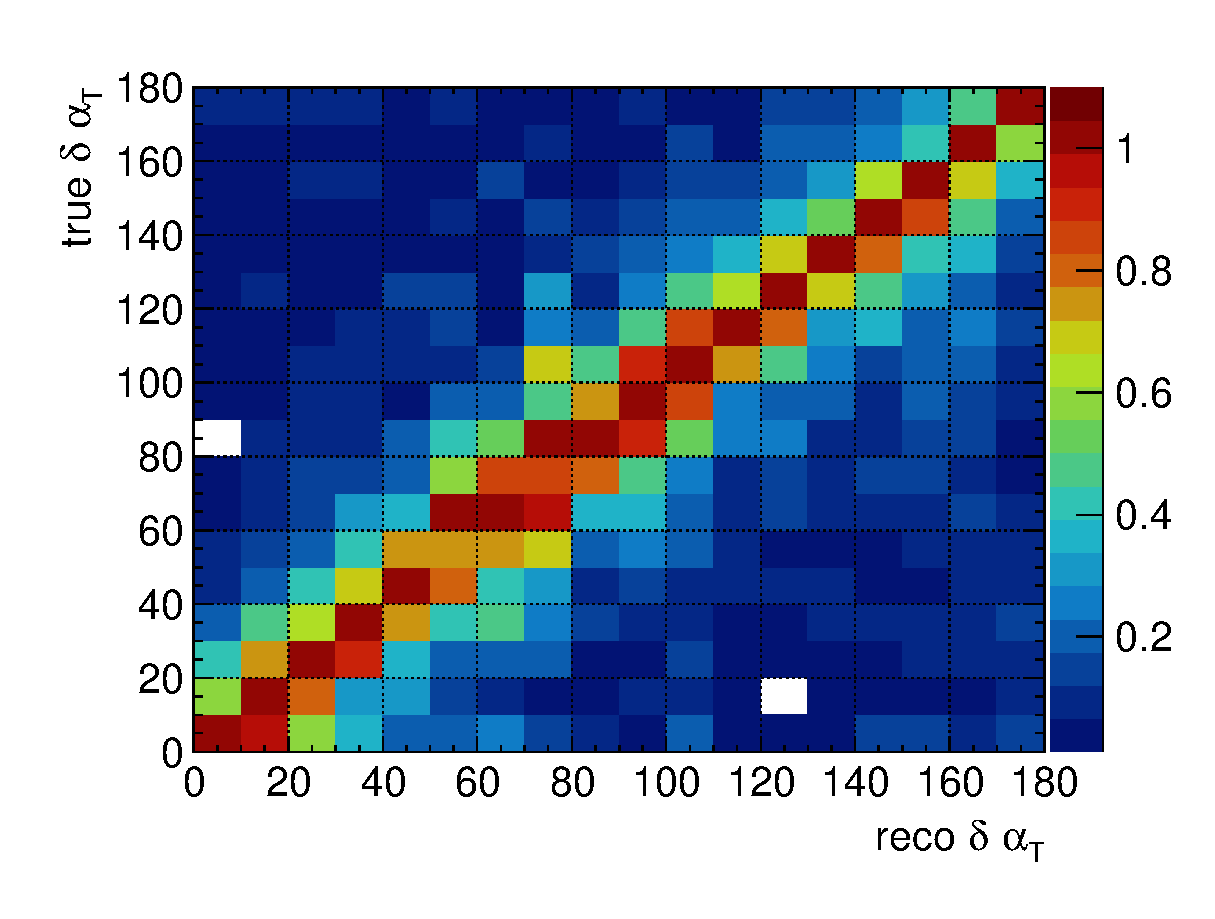
\includegraphics[width=\textwidth]{figures/perf/tki/dalphat_colnor_resmat_al13.eps}
               \caption{$\dat$ before ESC}
               \label{subfig:esc-dalpha-bfesc}
          \end{subfigure}
          \begin{subfigure}[b]{\dbfigwid\textwidth}
               \centering
               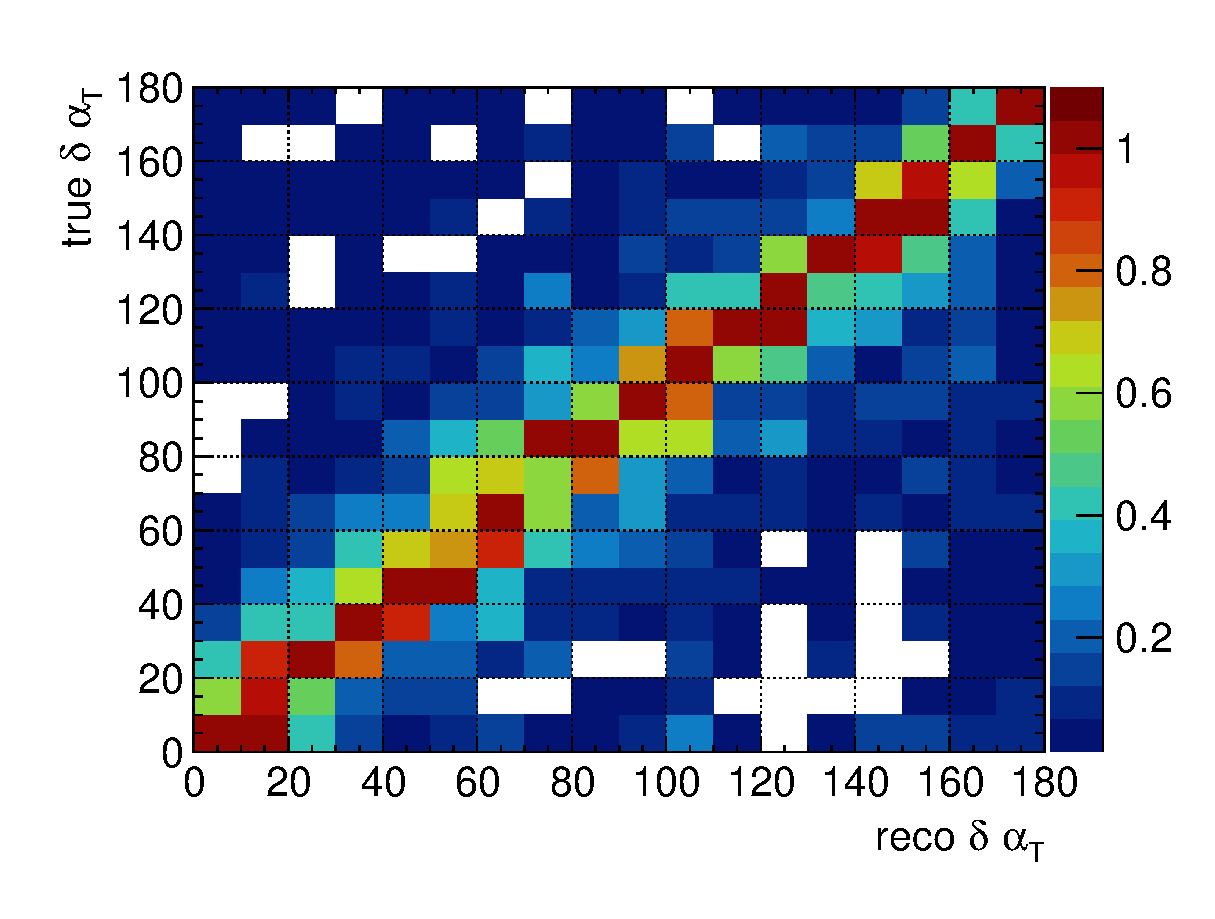
\includegraphics[width=\textwidth]{figures/perf/tki/dalphat_colnor_resmat_al14.eps}
               \caption{$\dat$ after ESC}
               \label{subfig:esc-dalpha-afesc}
          \end{subfigure}
          \\
          \begin{subfigure}[b]{\dbfigwid\textwidth}
               \centering
               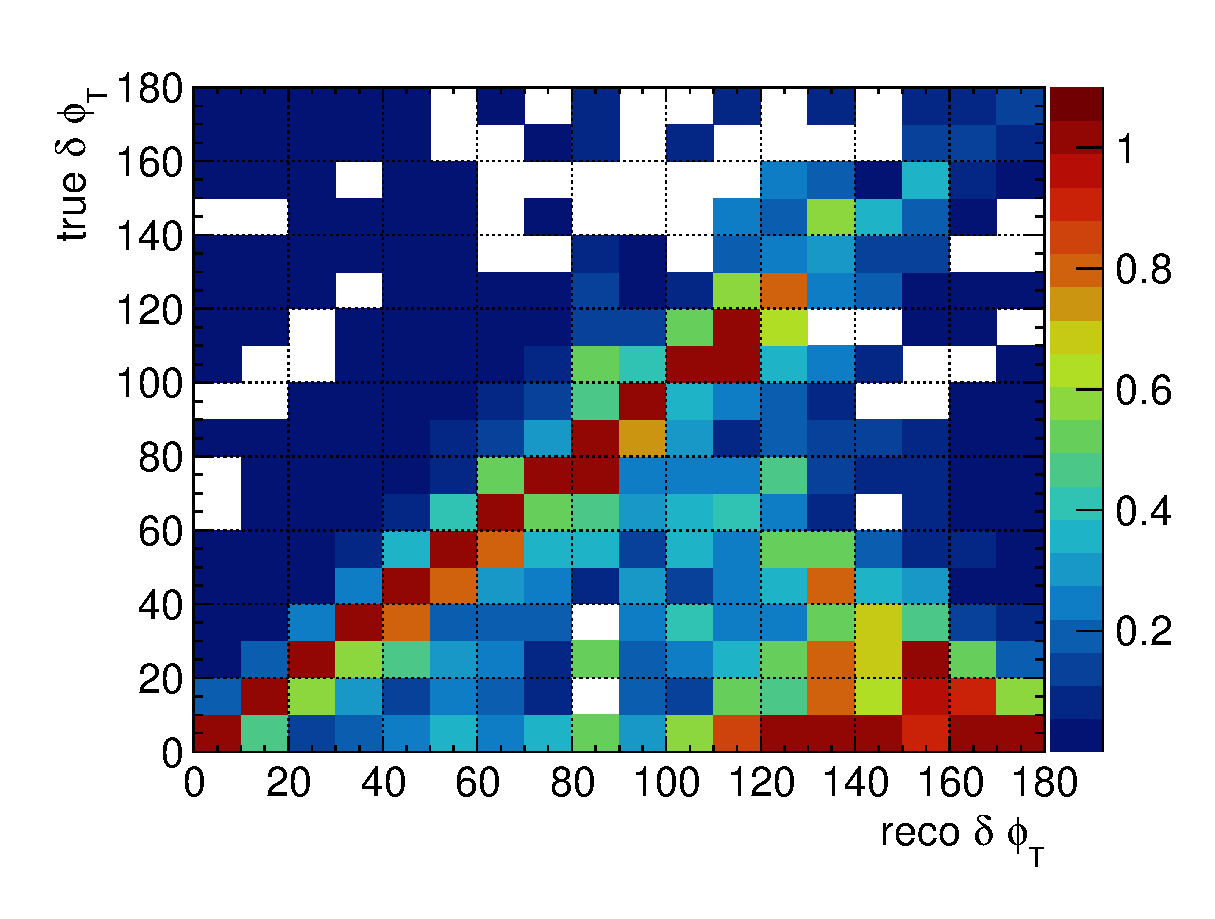
\includegraphics[width=\textwidth]{figures/perf/tki/dphitcolnor_resmat_al13.eps}
               \caption{$\dphit$ before ESC}
               \label{subfig:esc-dphit-bfesc}
          \end{subfigure}
          \begin{subfigure}[b]{\dbfigwid\textwidth}
               \centering
               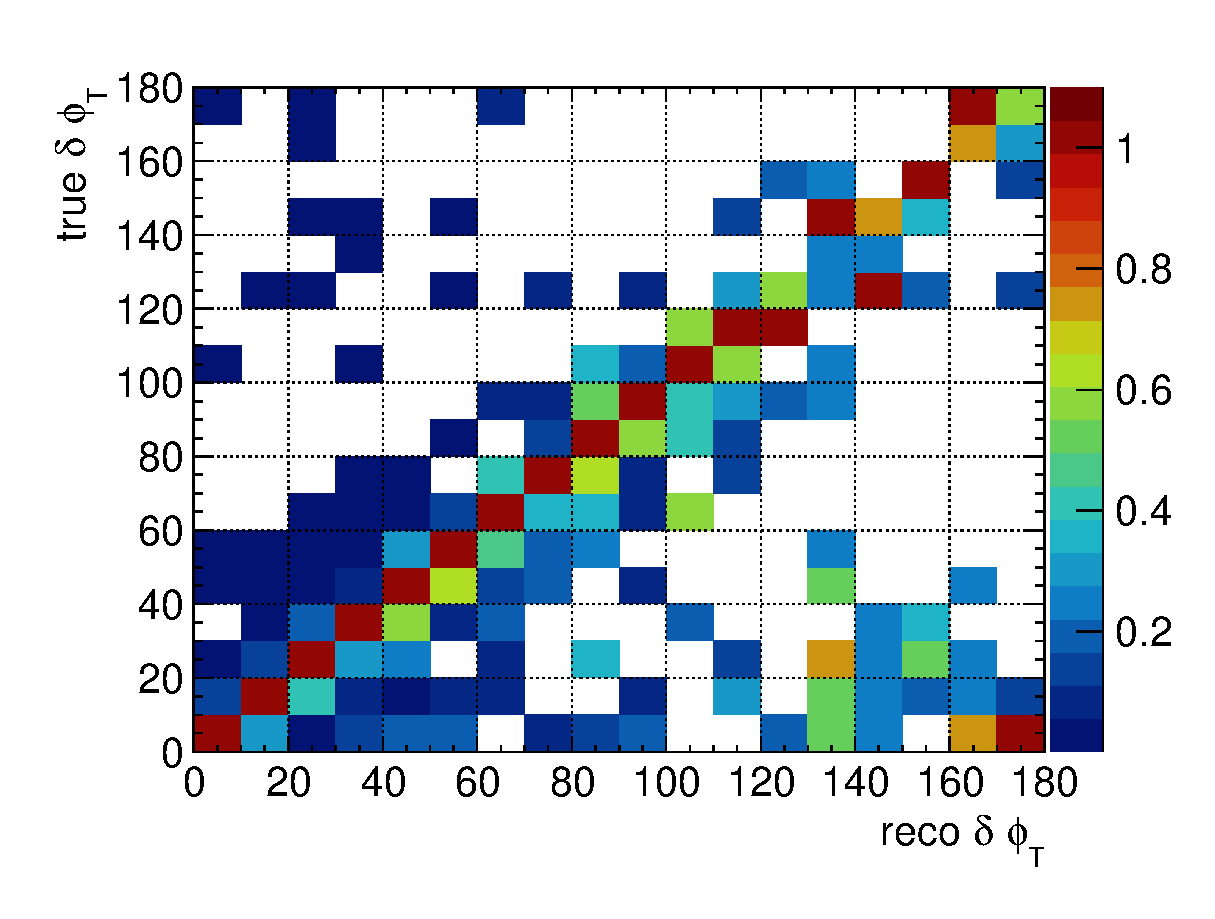
\includegraphics[width=\textwidth]{figures/perf/tki/dphitcolnor_resmat_al14.eps}
               \caption{$\dphit$ after ESC}
               \label{subfig:esc-dphit-afesc}
          \end{subfigure}
          \\
          \begin{subfigure}[b]{\dbfigwid\textwidth}
               \centering
               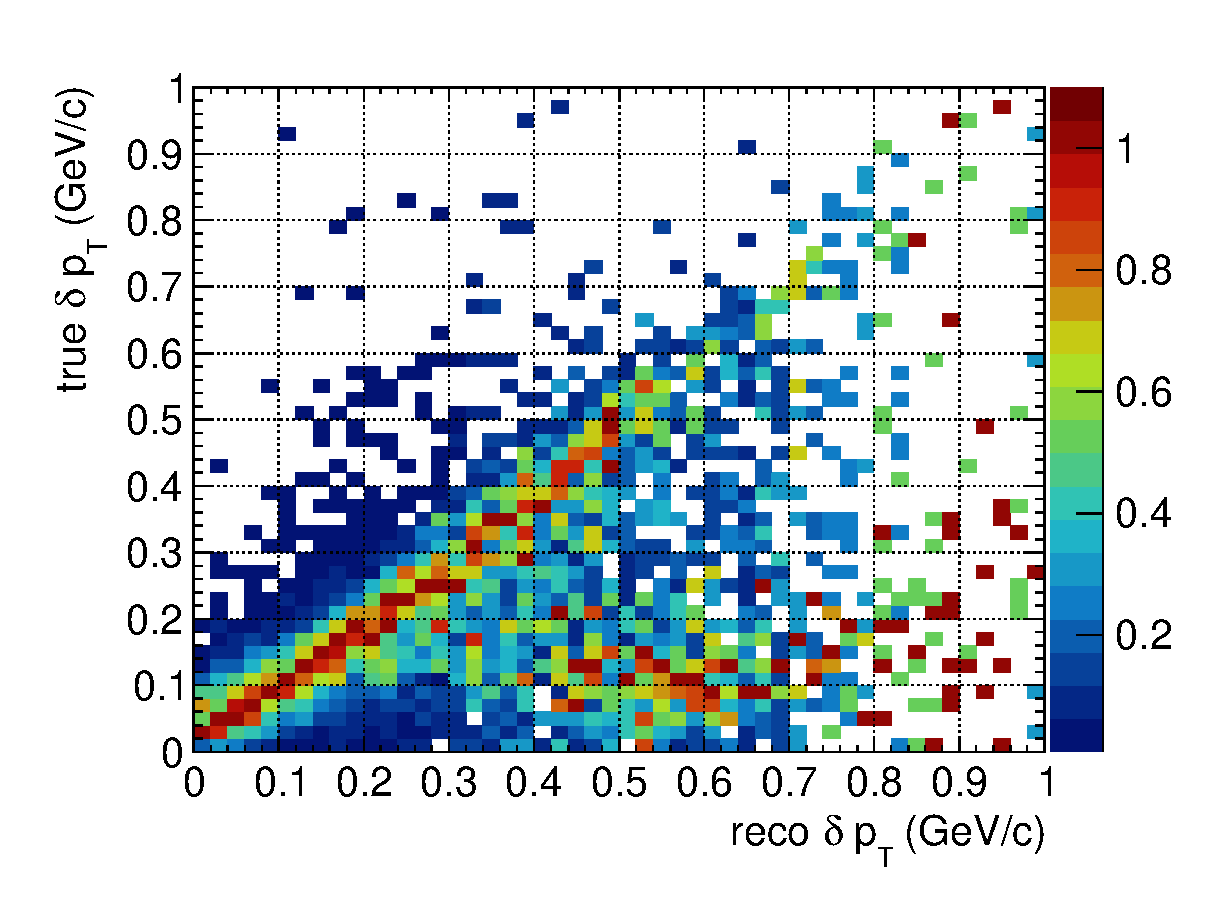
\includegraphics[width=\textwidth]{figures/perf/tki/dpt_colnor_resmat_al13.eps}
               \caption{$\dpt$ before ESC}
               \label{subfig:esc-dpt-bfesc}
          \end{subfigure}
          \begin{subfigure}[b]{\dbfigwid\textwidth}
               \centering
               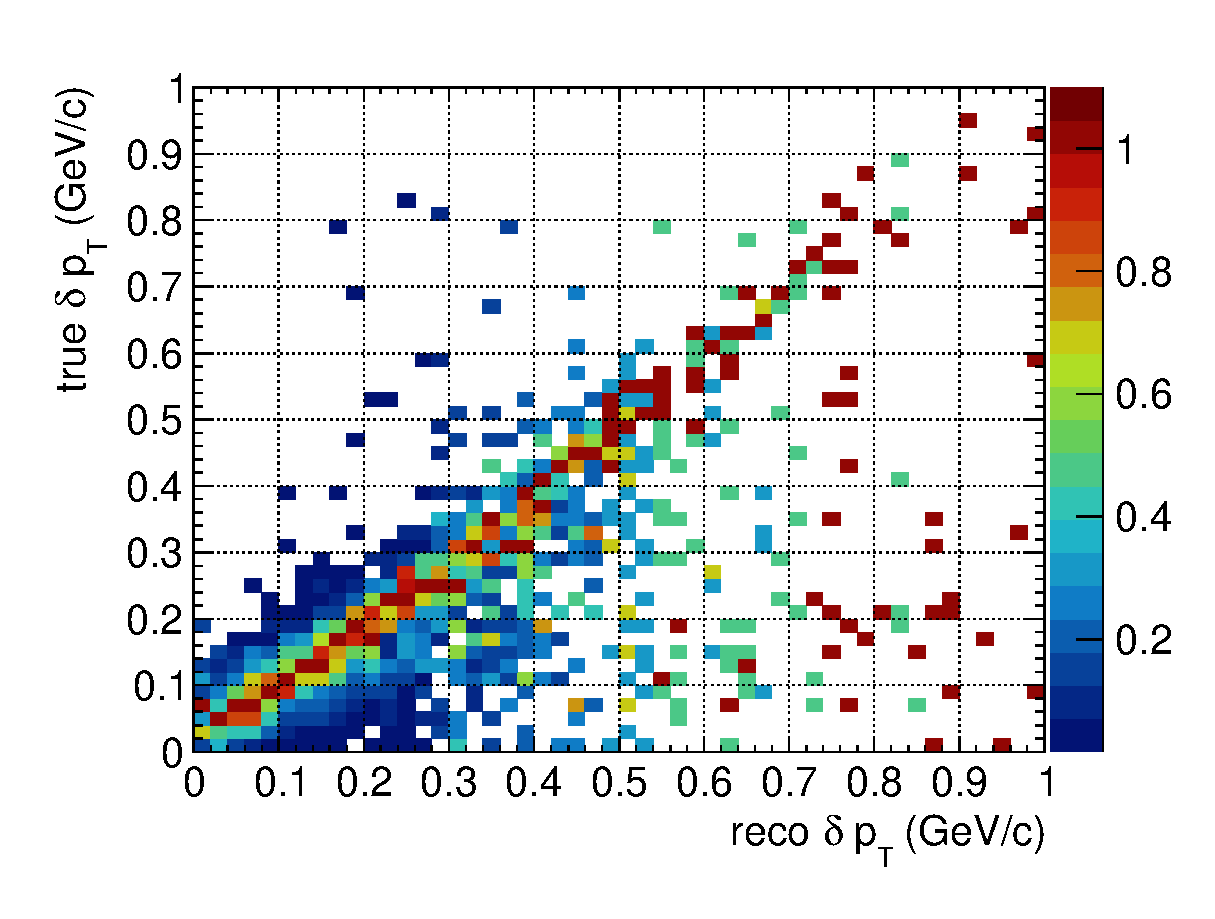
\includegraphics[width=\textwidth]{figures/perf/tki/dpt_colnor_resmat_al14.eps}
               \caption{$\dpt$ after ESC}
               \label{subfig:esc-dpt-afesc}
          \end{subfigure}
          \\
          \begin{subfigure}[b]{\dbfigwid\textwidth}
               \centering
               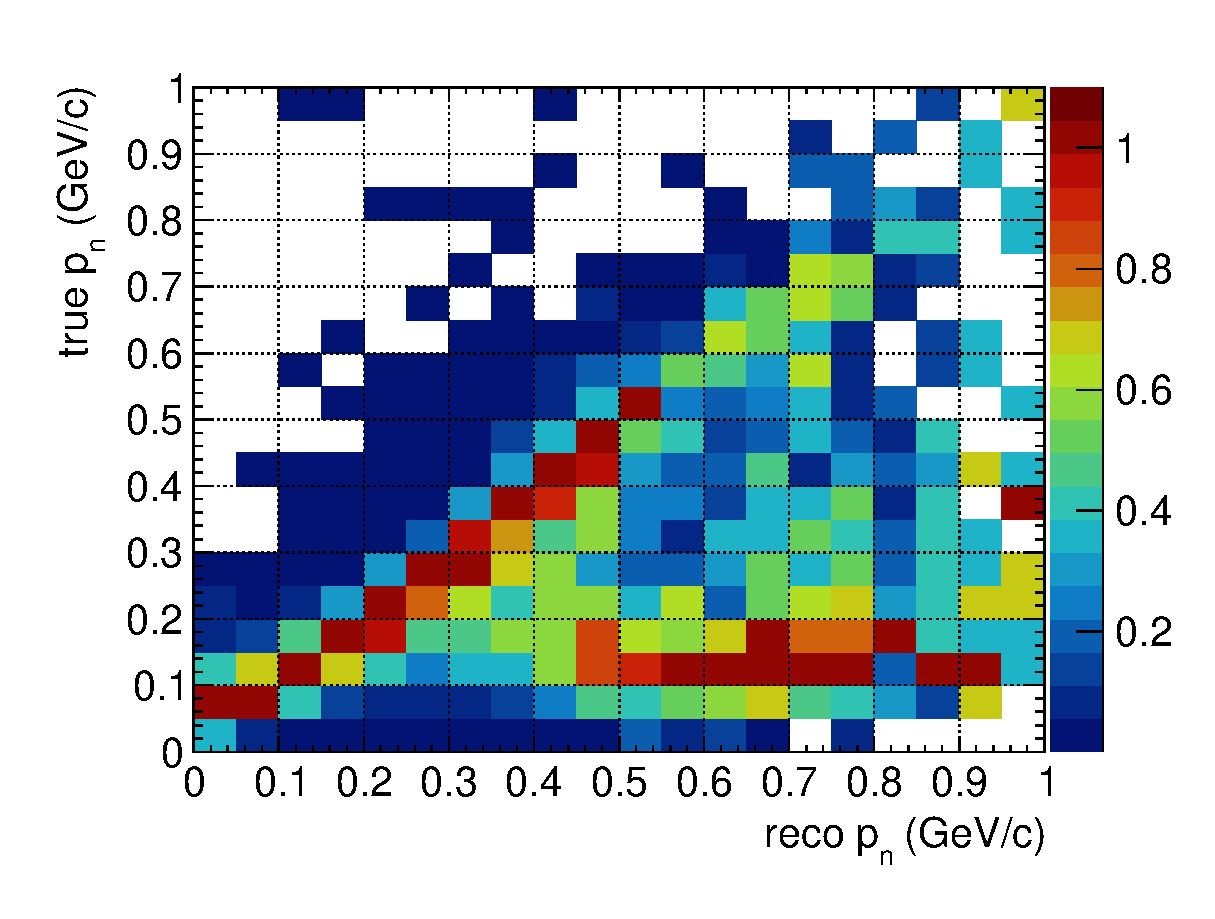
\includegraphics[width=\textwidth]{figures/perf/tki/pn_colnor_resmat_al13.eps}
               \caption{$\pn$ before ESC}
               \label{subfig:esc-pn-bfesc}
          \end{subfigure}
          \begin{subfigure}[b]{\dbfigwid\textwidth}
               \centering
               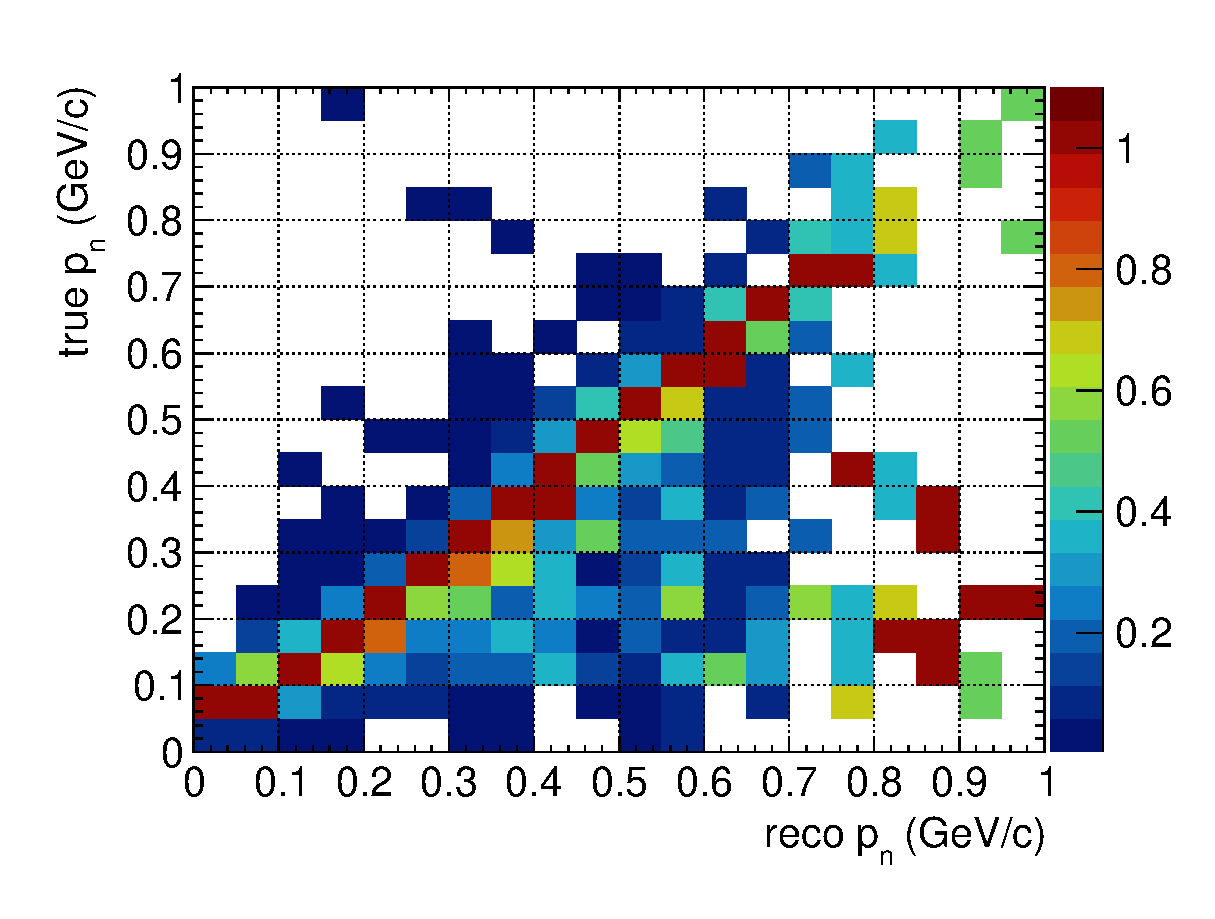
\includegraphics[width=\textwidth]{figures/perf/tki/pn_colnor_resmat_al14.eps}
               \caption{$\pn$ after ESC}
               \label{subfig:esc-pn-afesc}
          \end{subfigure}
          \caption{TKI variables before and after ESC for the $\numucczpiop$ selection.}
          \label{fig:mc-tki-0pi-esc}
     \end{figure}

     The impact of the muon momentum bias correction is best illustrated with a resolution fit in Fig.~\ref{fig:mc-tki-0pi-mubias}.
     This correction has a negligible impact on the angular variables, but it helps reduce bias in the momentum variables.
     As shown in Fig.~\ref{subfig:esc-dpt-bfmu} and Fig.~\ref{subfig:esc-dpt-afmu}, the $\dpt$ fitted mean improves from $0.92$ to $0.95$ after the muon bias correction.
     Similarly, in Fig.~\ref{subfig:esc-pn-bfmu} and Fig.~\ref{subfig:esc-pn-afmu}, the $\pn$ fitted mean improves from $0.94$ to $1.01$.
     This reduction in bias can also be observed in the decreased overestimated tails in the $\dpt$ and $\pn$ distributions.
     \begin{figure}
          \begin{subfigure}[b]{\dbfigwid\textwidth}
               \centering
               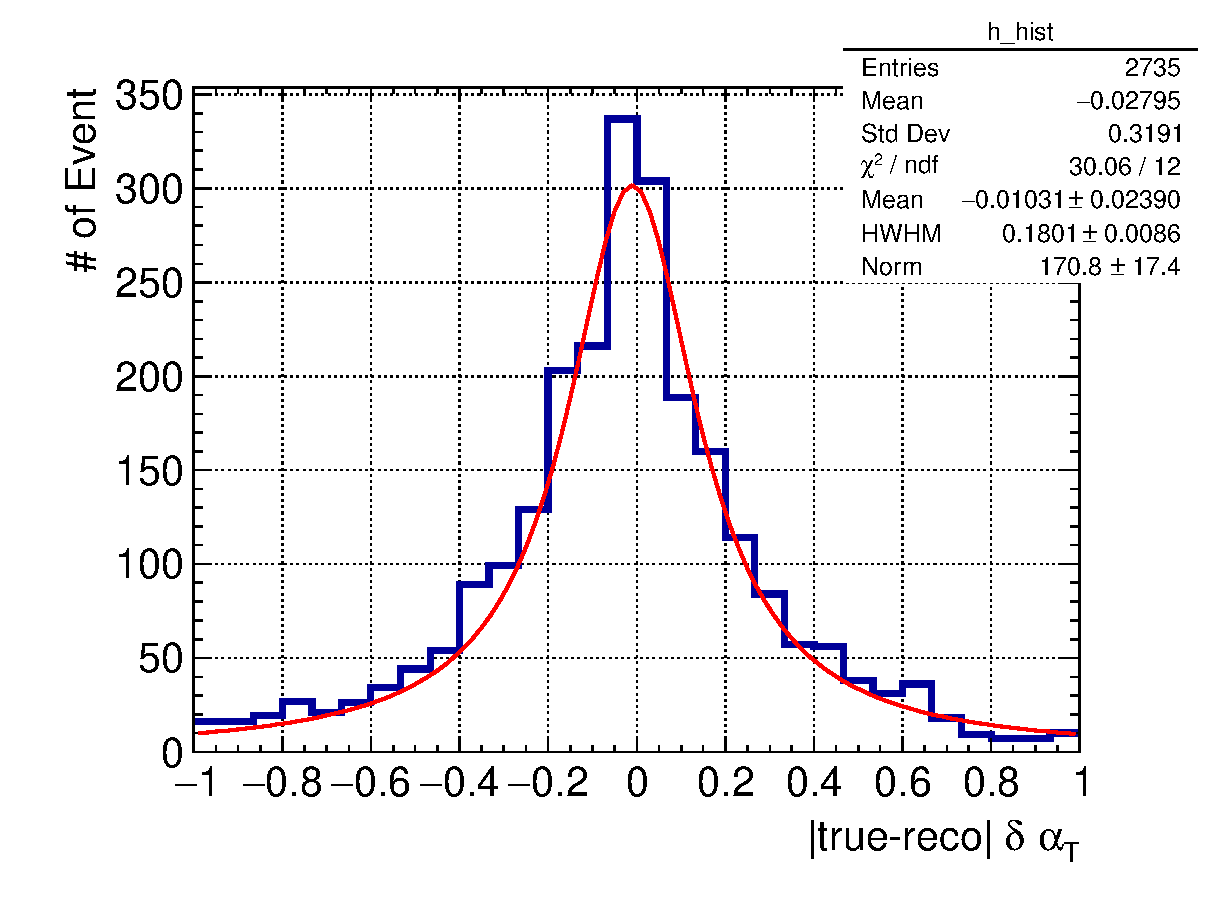
\includegraphics[width=\textwidth]{figures/perf/tki/dalphat_rat_hist_al14.eps}
               \caption{$\dat$ before muon bias correction}
               \label{subfig:esc-dalpha-bfmu}
          \end{subfigure}         
          \begin{subfigure}[b]{\dbfigwid\textwidth}
               \centering
               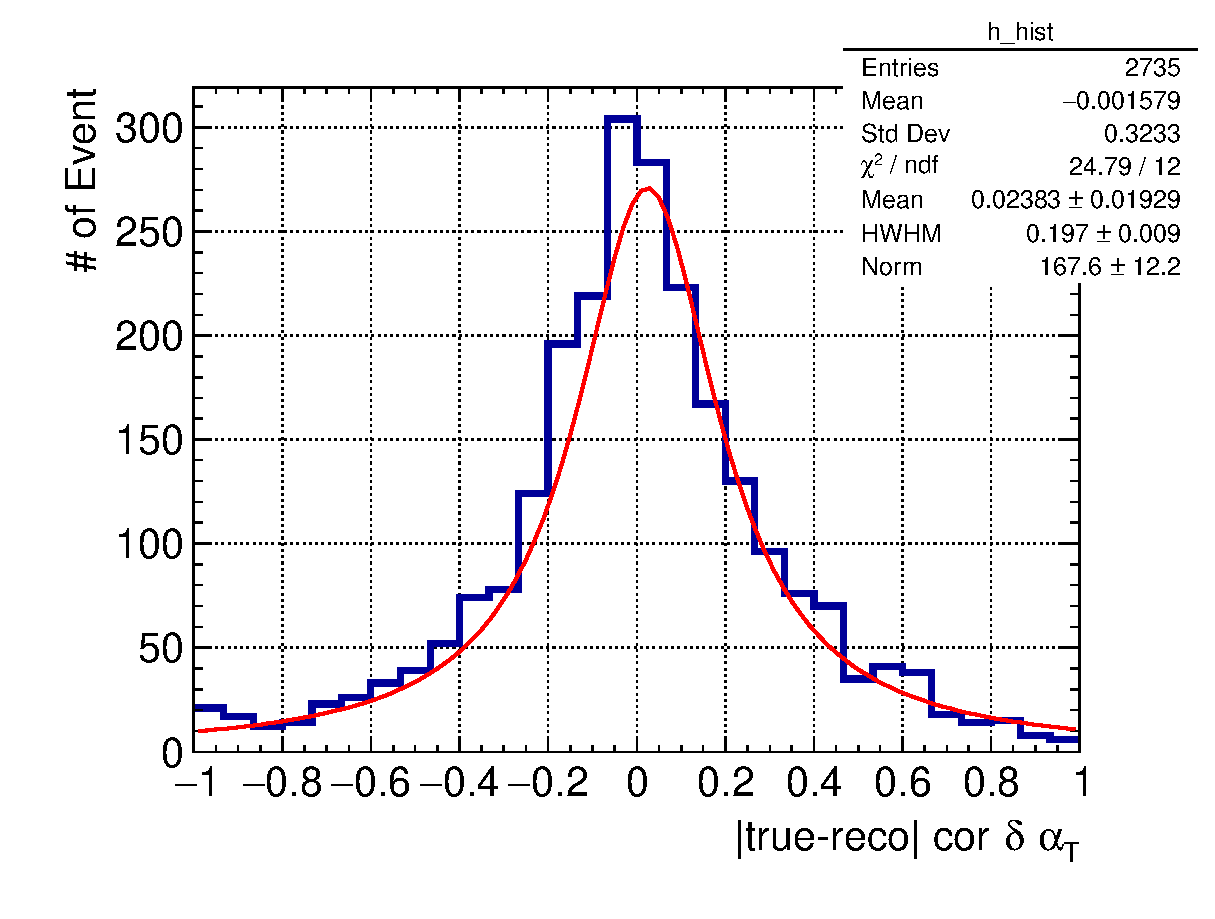
\includegraphics[width=\textwidth]{figures/perf/tki/cor_dalphat_rat_hist_al14.eps}
               \caption{$\dat$ after muon bias correction}
               \label{subfig:esc-dalpha-afmu}
          \end{subfigure}         
          \\
          \begin{subfigure}[b]{\dbfigwid\textwidth}
               \centering
               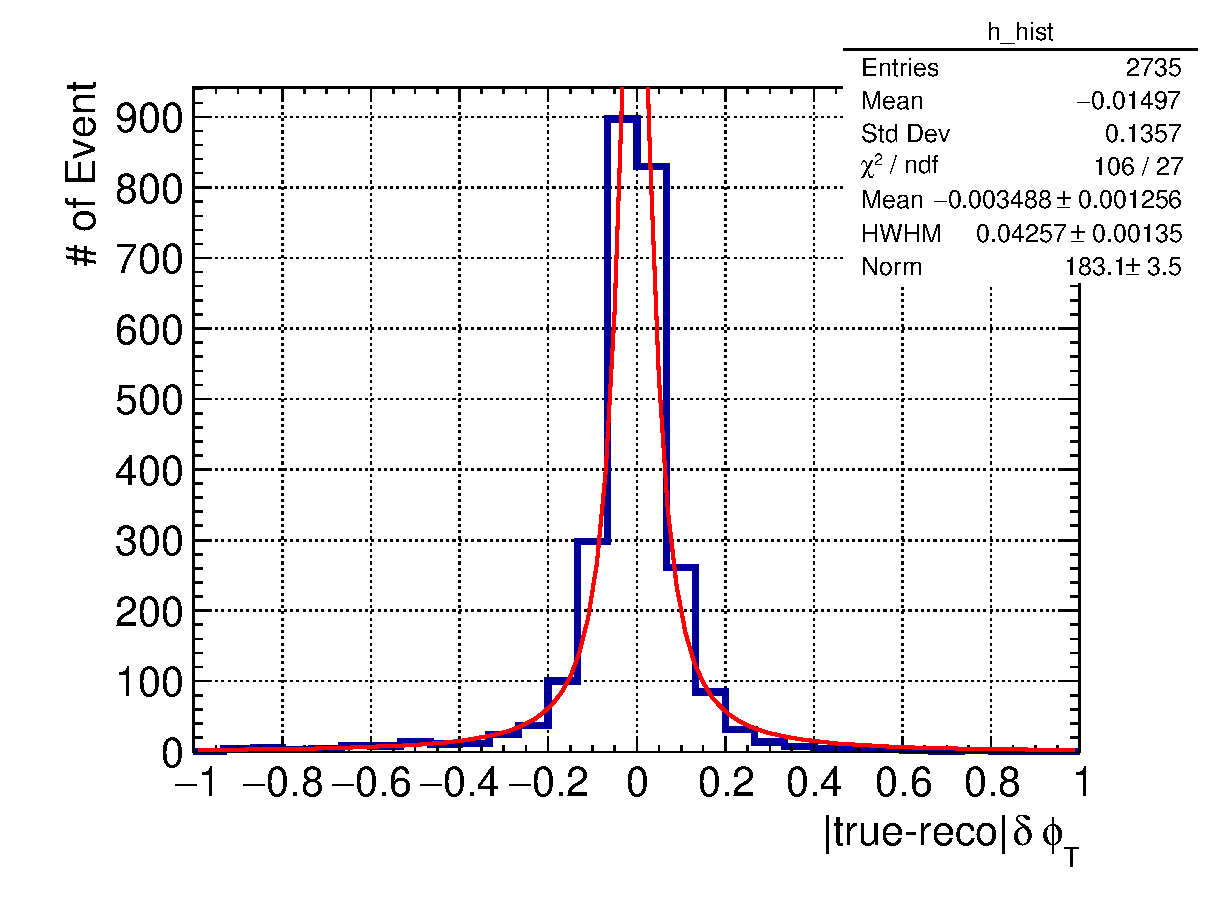
\includegraphics[width=\textwidth]{figures/perf/tki/dphit_rat_hist_al14.eps}
               \caption{$\dphit$ before muon bias correction.}
               \label{subfig:esc-dphit-bfmu}
          \end{subfigure}
          \begin{subfigure}[b]{\dbfigwid\textwidth}
               \centering
               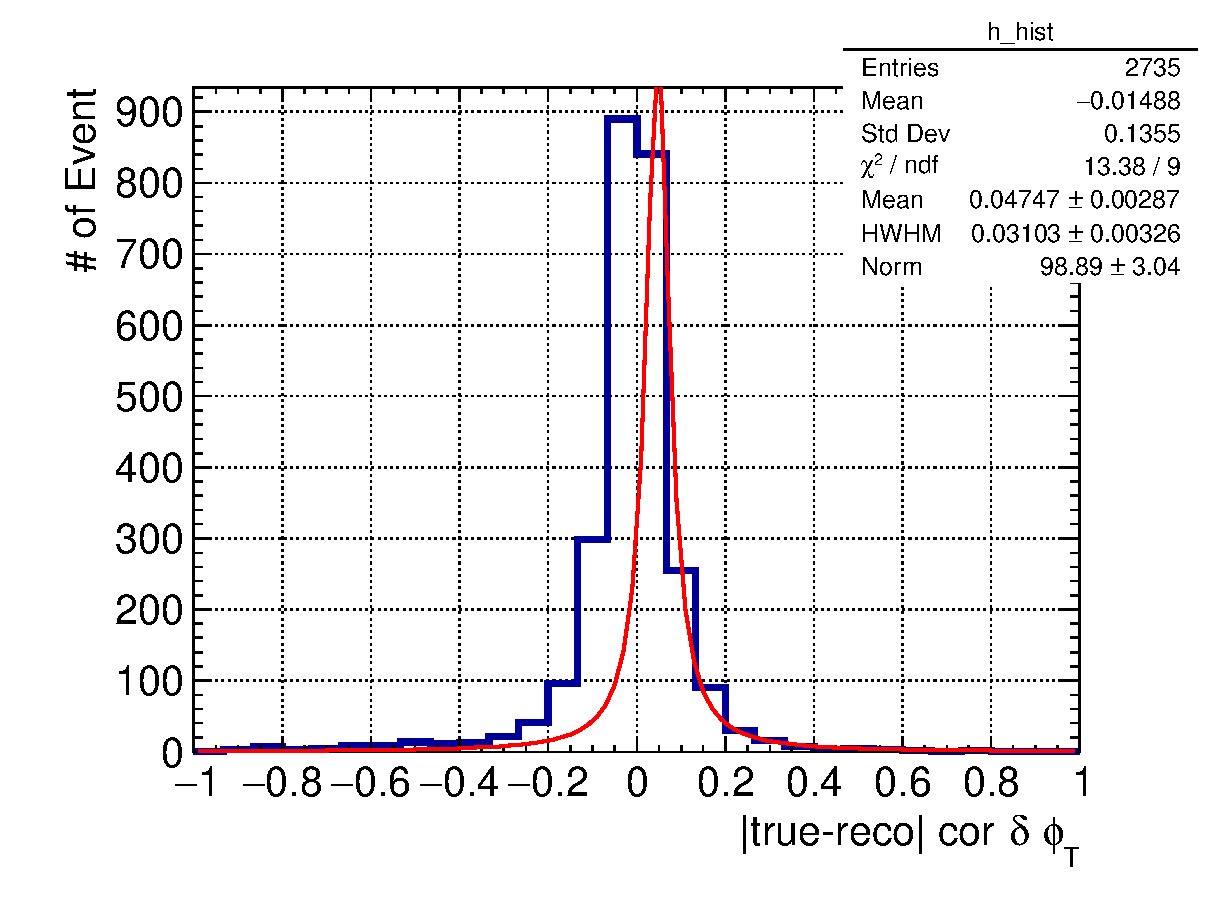
\includegraphics[width=\textwidth]{figures/perf/tki/cor_dphit_rat_hist_al14.eps}
               \caption{$\dphit$ after muon bias correction.}
               \label{subfig:esc-dphit-afmu}
          \end{subfigure}
          \\
          \begin{subfigure}[b]{\dbfigwid\textwidth}
               \centering
               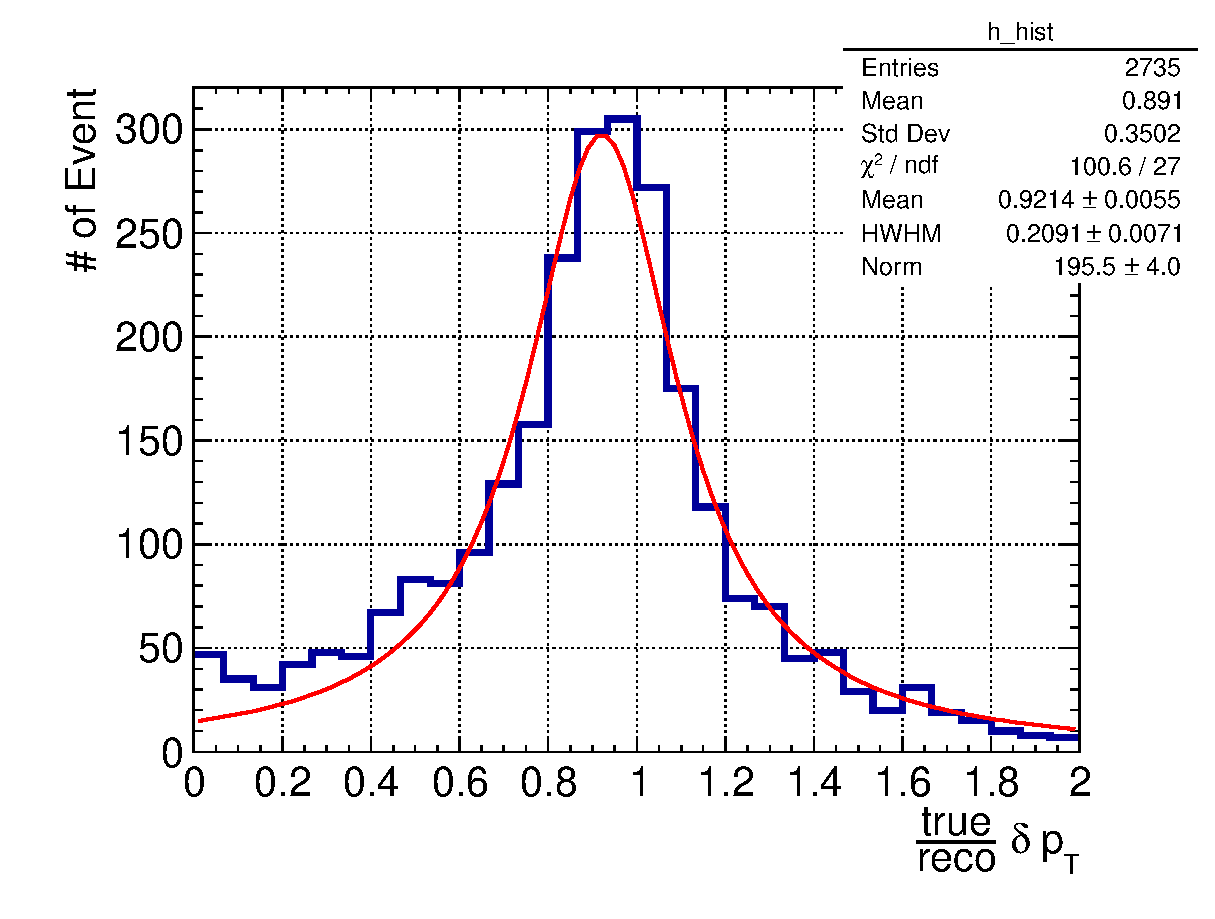
\includegraphics[width=\textwidth]{figures/perf/tki/dpt_rat_hist_al14.eps}
               \caption{$\dpt$ before muon bias correction}
               \label{subfig:esc-dpt-bfmu}
          \end{subfigure}
          \begin{subfigure}[b]{\dbfigwid\textwidth}
               \centering
               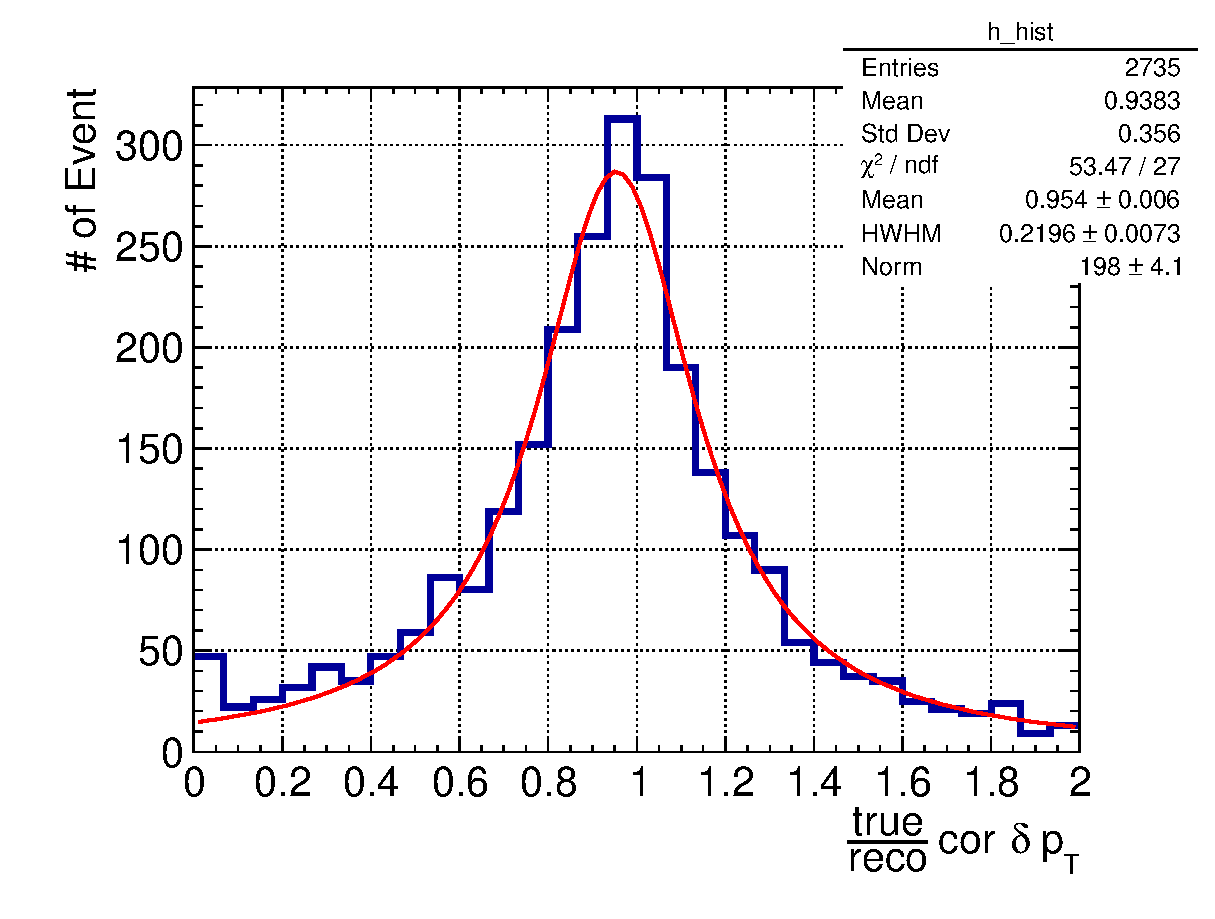
\includegraphics[width=\textwidth]{figures/perf/tki/cor_dpt_rat_hist_al14.eps}
               \caption{$\dpt$ after muon bias correction}
               \label{subfig:esc-dpt-afmu}
          \end{subfigure}
          \\
          \begin{subfigure}[b]{\dbfigwid\textwidth}
               \centering
               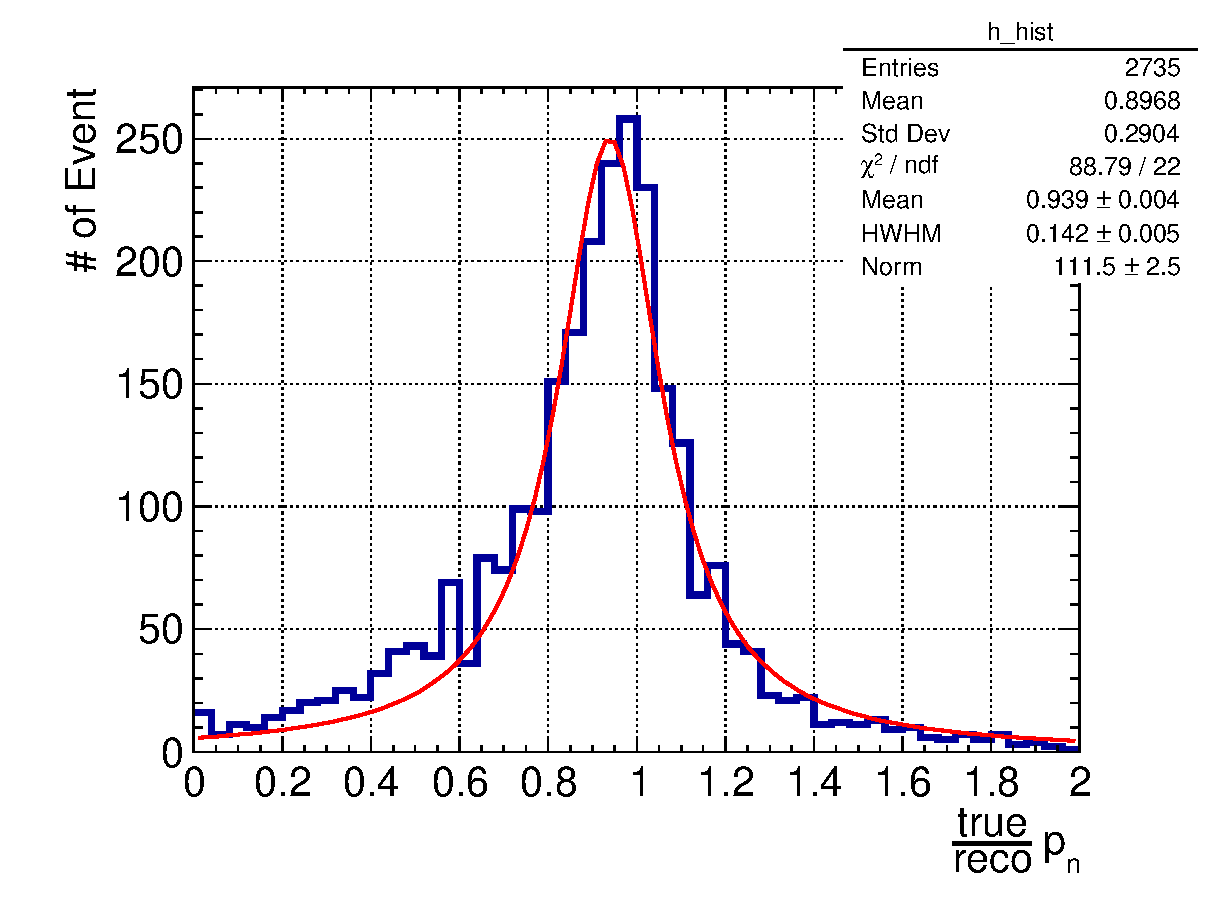
\includegraphics[width=\textwidth]{figures/perf/tki/pn_rat_hist_al14.eps}
               \caption{$\pn$ before muon bias correction}
               \label{subfig:esc-pn-bfmu}
          \end{subfigure}
          \begin{subfigure}[b]{\dbfigwid\textwidth}
               \centering
               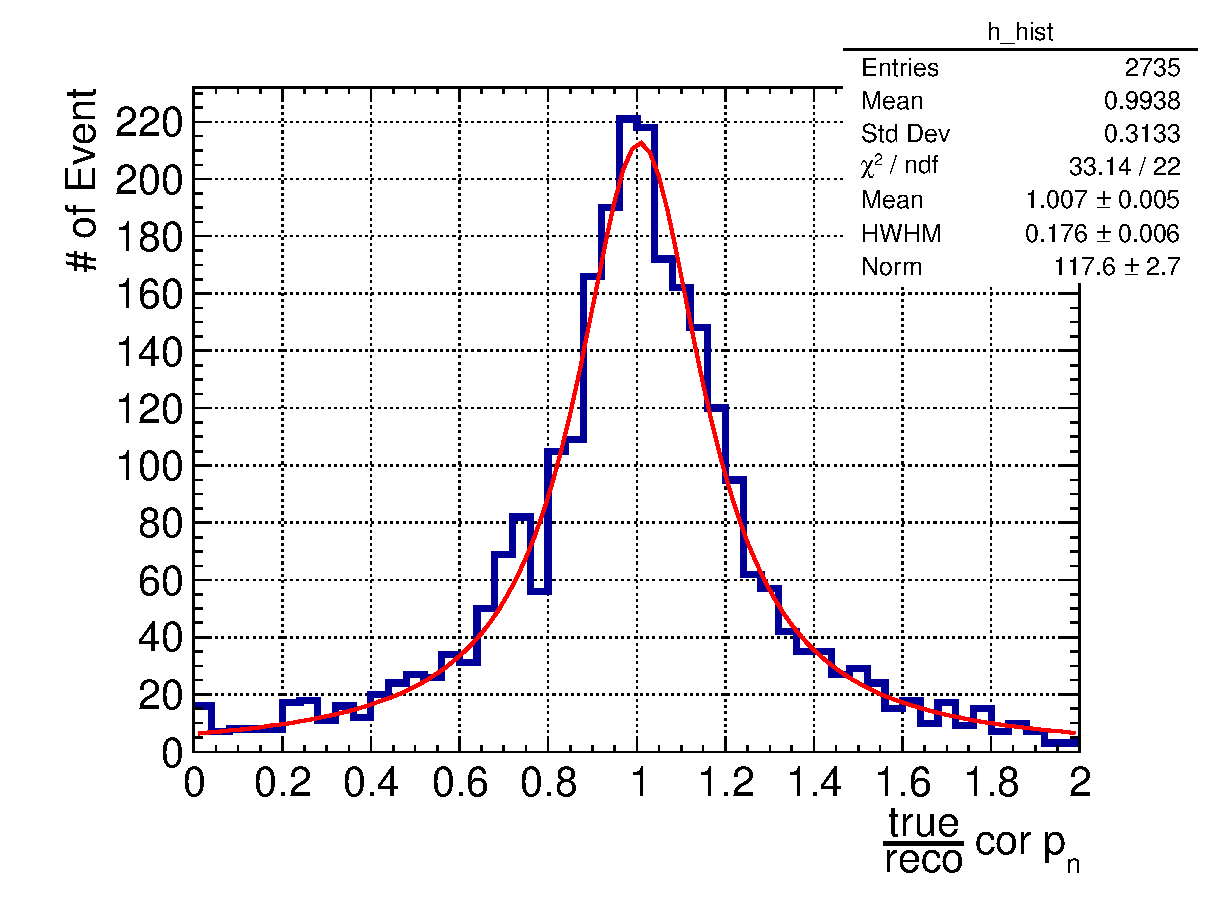
\includegraphics[width=\textwidth]{figures/perf/tki/cor_pn_rat_hist_al14.eps}
               \caption{$\pn$ after muon bias correction}
               \label{subfig:esc-pn-afmu}
          \end{subfigure}
          \caption{TKI variables before and after muon bias correction for the $\numucczpiop$ selection.}
          \label{fig:mc-tki-0pi-mubias}
     \end{figure}

     In Sec.~\ref{sec:sel-esc}, it was shown that the ESC technique improves proton momentum reconstruction resolution but diminishes efficiency by about $60\%$.
     The results in this section further highlight the necessity of the ESC technique for precise TKI measurements.
     With the ESC technique, the upgraded T2K ND can achieve high-resolution TKI measurements with minimal bias.
     Recently, an improved reconstruction algorithm enabled an updated TKI measurement at the pre-upgrade ND280.
     This yields a standard deviation of about $27\%$ for the $\pn$ reconstruction resolution.
     The resolution of $30\%$ for the TPC-$\mu$ sub-sample is comparable to this improvement, whereas the resolution of about $17\%$ for the SFGD-$\mu$ sub-sample is noticeably better as shown in Fig.~\ref{fig:sfgmu-0pi-pn}.
     There remains room for additional improvement in the upgraded measurement as the global reconstruction matures.
     \begin{figure}
          \centering
          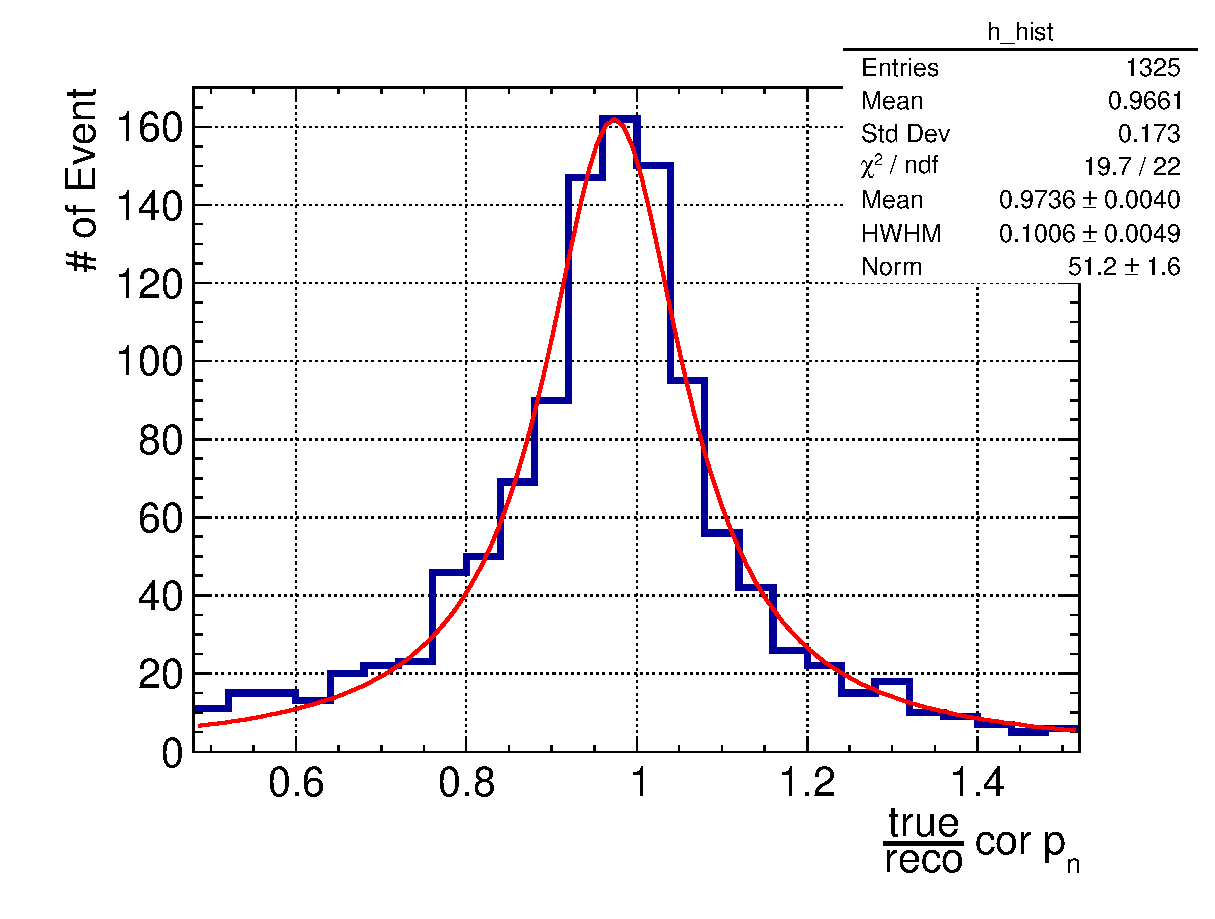
\includegraphics[width=\sgfigwid\textwidth]{figures/perf/tki/cor_pn_rat_hist_al11_sfgmu.eps}
          \caption{\label{fig:sfgmu-0pi-pn} $\pn$ distribution for the SFGD-$\mu$ sub-sample.}
     \end{figure}

     \subsection{$\numuccopiop$ selection}
     \label{sec:mc-tki-1pi}
     The $\numuccopiop$ selection uses the pion trackless reconstruction technique as elaborated in Sec.~\ref{sec:sel-tl} for the $\numuccopi$-TL selection.
     Additionally, it requires the reconstruction of one ESC proton.
     Hence, this sample uses both novel techniques in Chapter~\ref{ch:techniques}, showcasing the potential of the upgraded ND280 detector in hadronic measurements.

     The TKI variables for the $\numuccopiop$ selection are shown in Fig.~\ref{fig:mc-tki-1pi}, with even better resolution than the $\numucczpiop$-ESC selection.
     For example, Fig.~\ref{subfig:1pi-pn} shows a fitted HWHM of $12\%$, significantly than either of the sub-samples shown in the previous section.
     This improvement could be due to a purer sample due to the requirment of the presence of the extra pion.
     However, considerbale underestimation is observed for $\dpt$ in Fig.~\ref{subfig:1pi-dpt}, which is surprising given the good performance of the other TKI variables.
     This could be due to a bug in the recconstruction, but as the current reconstruction software has become obsolete, this issue will be furthere investigated when the new and stable reconstruction become available.
     Nevertheless, the excellent resolutions shown in other TKI variables demonstrate a potential for the upgraded ND280 detector to achieve high-precision TKI measurements.
     The same workflow of the ESC technique and muon momentum bias correction can be applied to the future software, while keeping in mind of the unexpected behavior in $\dpt$.
     \begin{figure}
          \begin{subfigure}[b]{\dbfigwid\textwidth}
               \centering
               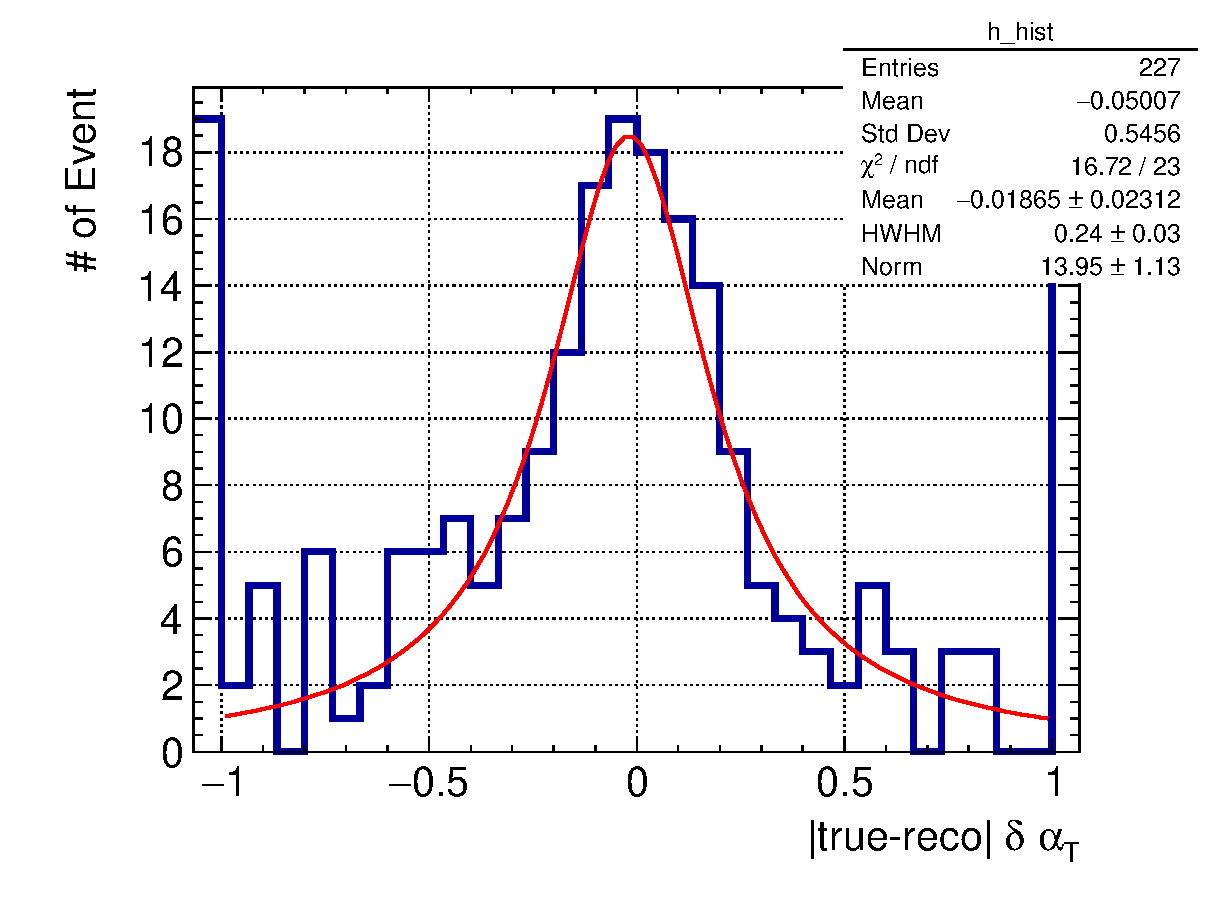
\includegraphics[width=\textwidth]{figures/perf/tki/SFGpTPCmu_dalphat_rat_hist_al14.eps}
               \caption{$\dat$}
               \label{subfig:1pi-dalpha}
          \end{subfigure}         
          \begin{subfigure}[b]{\dbfigwid\textwidth}
               \centering
               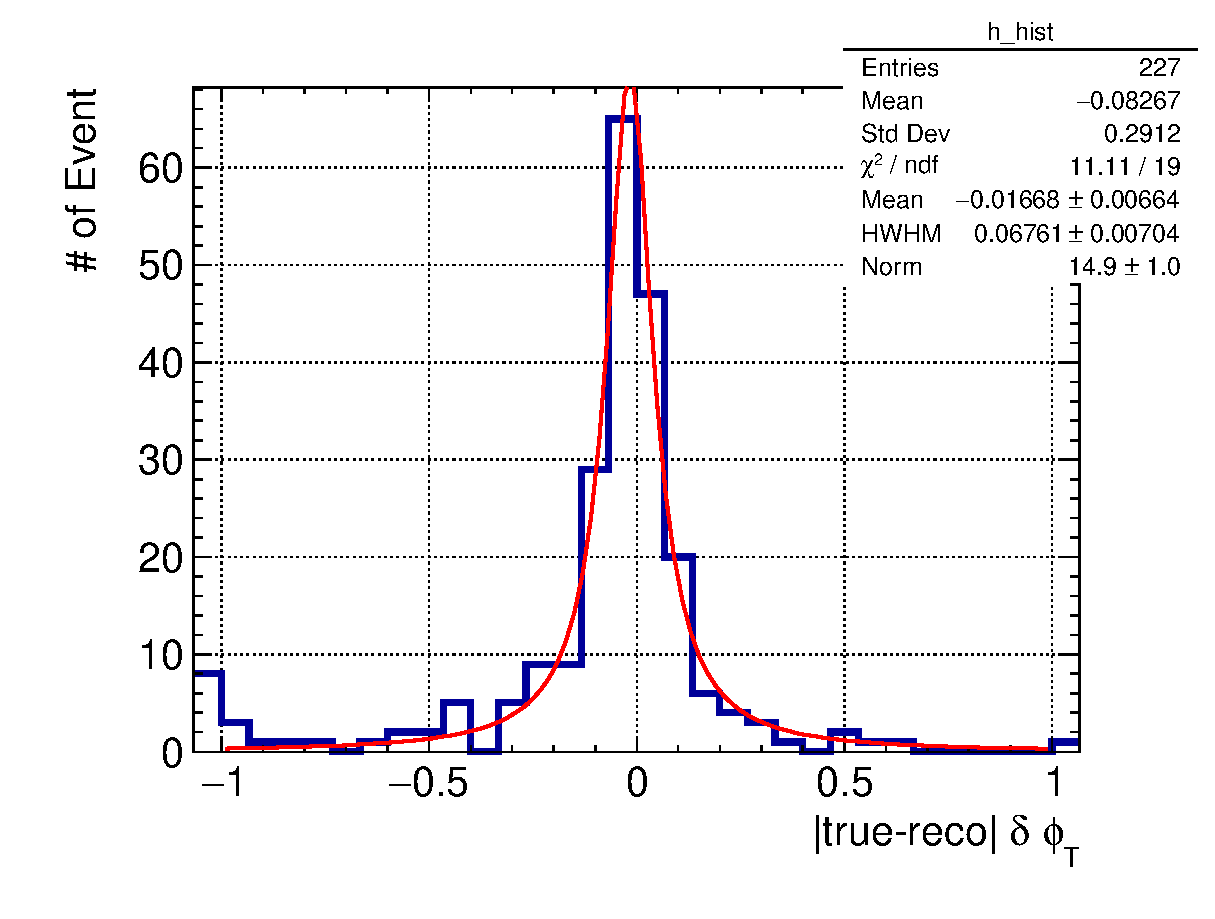
\includegraphics[width=\textwidth]{figures/perf/tki/SFGpTPCmu_dphit_rat_hist_al14.eps}
               \caption{$\dphit$}
               \label{subfig:1pi-dphit}
          \end{subfigure}
          \\
          \begin{subfigure}[b]{\dbfigwid\textwidth}
               \centering
               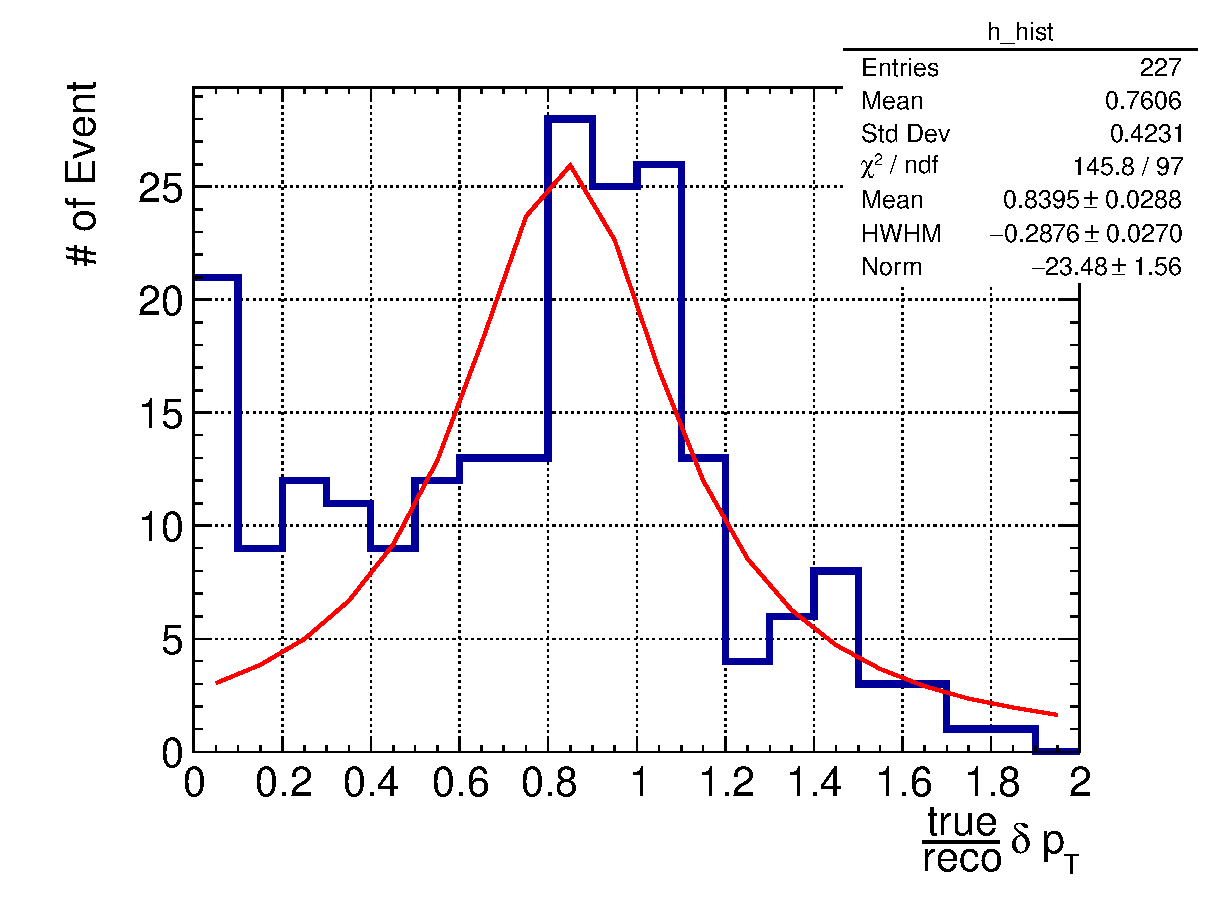
\includegraphics[width=\textwidth]{figures/perf/tki/SFGpTPCmu_dpt_rat_hist_al14.eps}
               \caption{$\dpt$}
               \label{subfig:1pi-dpt}
          \end{subfigure}
          \begin{subfigure}[b]{\dbfigwid\textwidth}
               \centering
               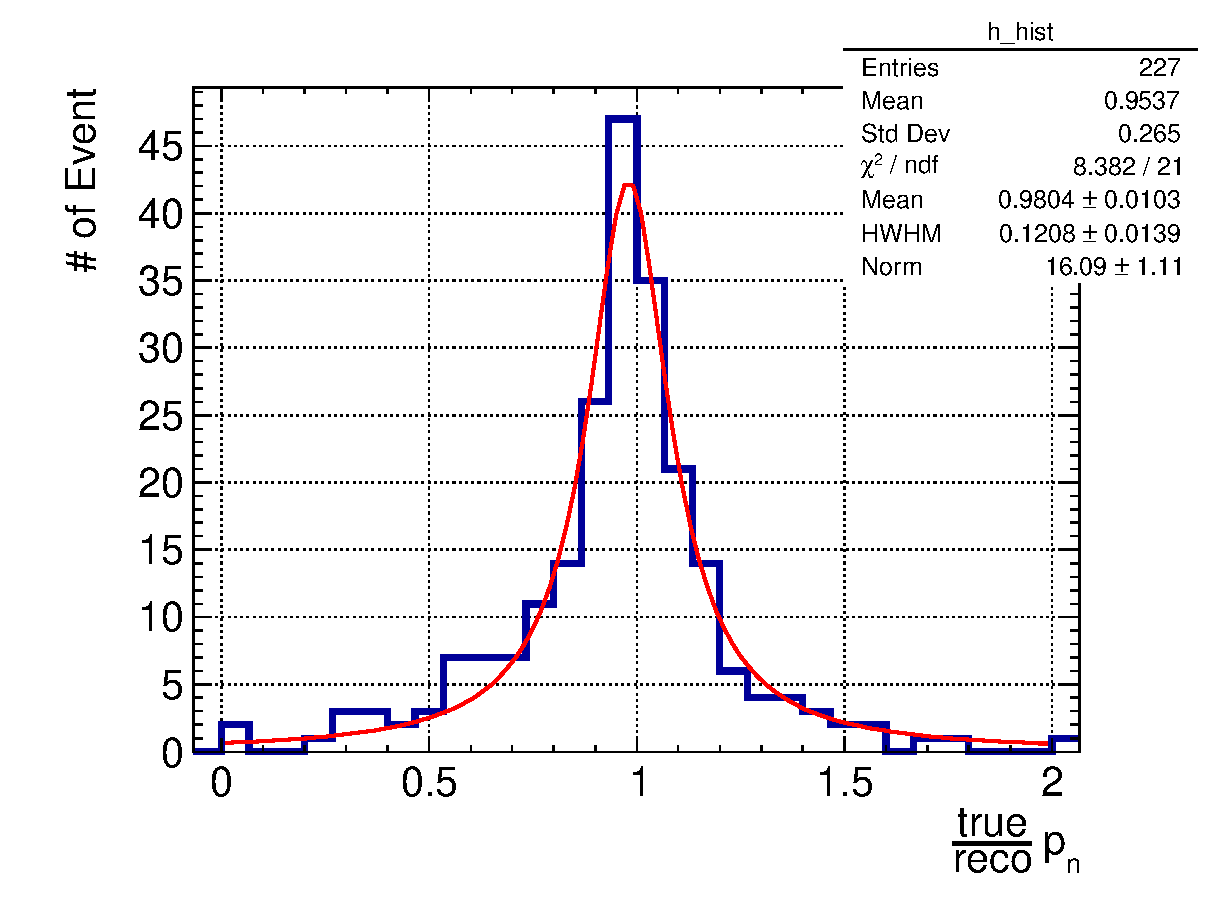
\includegraphics[width=\textwidth]{figures/perf/tki/SFGpTPCmu_pn_rat_hist_al14.eps}
               \caption{$\pn$}
               \label{subfig:1pi-pn}
          \end{subfigure}
          \caption{TKI variables for the $\numuccopiop$ selection.}
          \label{fig:mc-tki-1pi}
     \end{figure}

     In addition to the single transverse variables presented above, the $\numuccopiop$ sample can also be used to measure the double transverse variable, $\dptt$, the net momentum transverse to both the neutrino momentum and the muon momentum.
     Without FSI, $\dptt$ should be $0$. 
     This special property can be exploited to select $\nu$-H events amidst $\nu$-C events as suggested in Ref.~\cite{Lu:2015hea}. 
     Hence, the main figure of merit for $\dptt$ measurement is the width of its distribution for $\nu$-H events, where the hydrogen events are picked by an additional check on the MC truth information.
     As shown in Fig.~\ref{fig:1pi-tki-dptt}, the fitted half width is about $12~\mevc$, which is significantly improved compared to $21~\mevc$, the pre-upgrade ND280 result~\cite{Lu:2015hea}, suggesting a greater potential to apply it for a hydrogen sample selection, which will be discussed at the end of this chapter in Sec.~\ref{sec:mc-hydrogen}.
     \begin{figure}[!htb] 
          \centering 		
          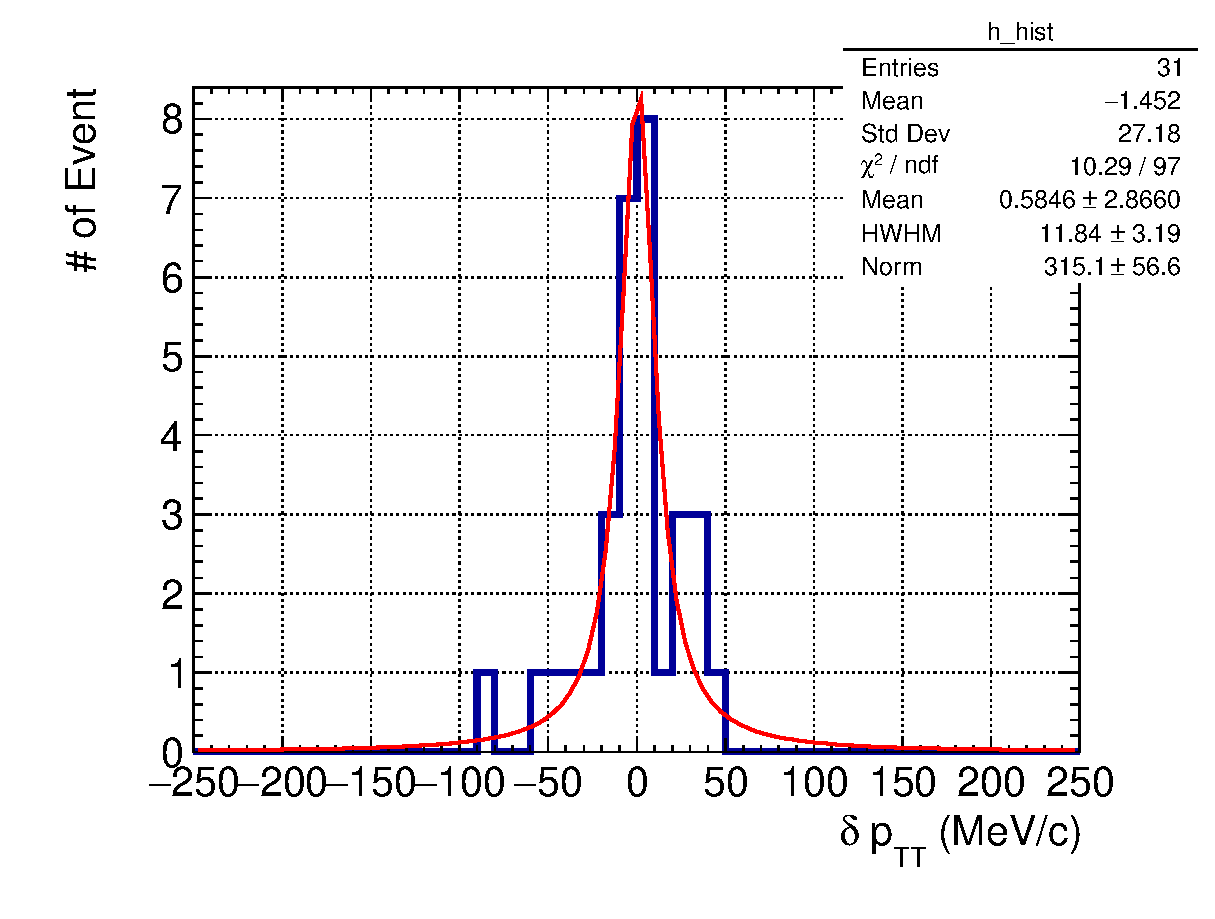
\includegraphics[width=\sgfigwid\textwidth]{figures/perf/tki/SFGpTPCmu_dptt_hist_al15_H_bin100_range500_Lfit.eps}
          \caption{\label{fig:1pi-tki-dptt} $\dptt$ distribution for $\nu$-H events.} 
     \end{figure}


\section{The COM Variables}
\label{sec:mc-com}
When a neutrino has sufficient energy, it can excite a nucleon into a resonance state, for example, the $\deltapp$. 
This process is referred to as a resonance (RES) interaction.
Since $\deltapp$ is one of the most commonly observed resonances in neutrino experiments, this work focuses on it as an example.
Nevertheless, the concept presented here is equally applicable to other resonances, and the methodology can be easily generalized.

The resonance decays rapidly, before leaving the nucleus, via the process
\begin{equation}
     \deltapp \rightarrow \pip + \p.
\end{equation}
In the $\deltapp$ rest frame, as illustrated in the top left of Fig.~\ref{fig:COM-diagram}, the kinematics of this two-body decay are well-defined, and the proton and pion are emitted back-to-back.
The pion decay angle, $\thetapidel$, is defined as the angle between $\vecppirest$ and the $x$-axis, which is taken to align with $\vecpdel$, the momentum of $\deltapp$ in the lab frame. 
$\thetapidel$ is a resonance property that follows an underlying distribution defined by various models~\cite{Rein:1987cb,Kabirnezhad:2017jmf,Kabirnezhad:2020wtp,Kabirnezhad:2022znc}.

\begin{figure}[ht!]
\centering
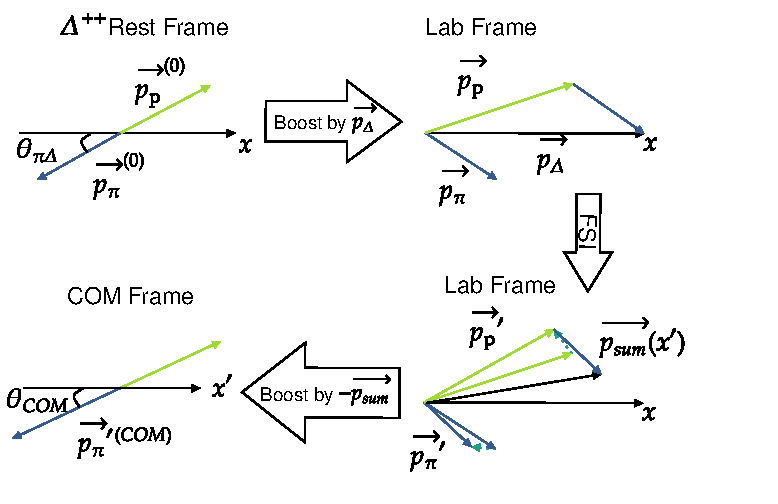
\includegraphics[width=\linewidth]{figures/COM/COM-diagram.pdf}
\caption{Schematic illustration of the COM angle. Without FSI, $\vecpsum=\vecpdel$ and the lab frame and the $\deltapp$ rest frame can be transformed into each other by $\vecpdel$. With FSI, $\vecpsum \neq \vecpdel$, the $\deltapp$ rest frame is not accessible, but the lab frame can be boosted into the COM frame using $\vecpsum$. Hence, the major difference of the COM frame from the $\deltapp$ rest frame is caused by FSI.}
\label{fig:COM-diagram}
\end{figure}

The kinematics in the lab frame are related to those in the $\deltapp$ rest frame by a boost with $\vecpdel$, as depicted in the top right of Fig.~\ref{fig:COM-diagram}. 
Without FSI, $\vecpdel$ equals the sum of $\vecpp$ and $\vecppi$.
However, the target materials of modern-day detectors are mainly comprised of nuclei with multiple nucleons, and FSI alters the kinematics of the hadrons considerably, as illustrated by the dotted arrows in the bottom right of Fig.~\ref{fig:COM-diagram}.

The altered momenta, $\vecppp$ and $\vecppip$, are the ones measured by detectors. 
Their sum generally differs from $\vecpdel$.
Thus, the $\deltapp$ rest frame, with its simple kinematic relations, becomes inaccessible.
Nevertheless, the system can be boosted to the proton-pion COM frame using $\vecpsum$, as depicted in the bottom left of Fig.~\ref{fig:COM-diagram}, where the $x^{\prime}$-axis is aligned with the $\vecpsum$ direction in the lab frame.
Similarly, a pion decay angle, $\thetacom$, can be defined between $\vecppicom$, the pion momentum in the COM frame, and the $x^{\prime}$-axis.
Due to FSI, $\thetacom$ typically differs from $\thetapidel$. 

The COM frame coincides with the $\deltapp$ rest frame only in the absence of FSI.
Thus, the strength of FSI dictates the deviation of $\thetacom$ from $\thetapidel$. 
In practice, the measured $\thetacom$ serves as a probe for studying FSI. 
$\thetapidel$, being a rest-frame property of $\deltapp$, is independent of the resonance's momentum, neutrino energy, and initial state (IS).
In neutrino event generators, $\thetacom$ deviates from $\thetapidel$ only due to FSI, which is independent of neutrino energy and IS.
Therefore, $\thetacom$ retains these important independencies.
As different resonances could have different decay properties, $\thetaR$, the similarly defined pion decay angle of a higher resonance $R$, generally differs from $\thetapidel$. 
Hence, $\thetacom$, a superposition of $\thetapidel$ and all possible $\thetaR$, will deviate from $\thetapidel$ when more resonances become energetically possible with an increase in neutrino energy. 
This deviation will be further elaborated in Sec.~\ref{sec:dis}.

Moreover, the total energy in the COM frame, $\ecom$, will be equal to the mass of the resonance in the absence of FSI.
Cutting on events with total energy far from the rest mass peak of the resonance will select events with minimal FSI effects, such as $\nu$-H events. 
The application of $\ecom$ for hydrogen event selection will be discussed in Sec.~\ref{sec:mc-hydrogen}.

Up to this point, the discussion of resonance decay has been entirely general and can thus be applied to and validated by various experiments, including hadron scattering measurements. 
However, there are features specific to neutrino experiments. 
First, the resonance is generated through neutrino-nucleon interactions, which involve both vector and axial currents. 
Second, the interaction occurs within the nuclear medium. 
This secion focuses on the latter, with the application of COM variables to the former is better elaborated in Sec.~\ref{sec:mc-hydrogen}.

While the COM angle may appear conceptually similar to the reconstructed Adler angle, $\thetaadt$, in neutrino experiments~\cite{Sanchez:2015yvw}, there are significant differences. 
Notably, the COM frame is reconstructed exclusively from hadronic kinematics, whereas the reconstructed Adler frame relies on leptonic kinematics and assumes stationary nucleons. 
Consequently, the reconstruction of the Adler frame is implicitly influenced by IS effects, whereas the COM frame's hadronic variables are impacted by final state interactions (FSI). 
Therefore, $\thetaadt$, being a hadronic variable in the Adler frame, is influenced by both IS and FSI. 
Additionally, the necessity of reconstructing the neutrino energy renders $\thetaadt$ sensitive to neutrino flux uncertainties, which are among the largest systematic uncertainties in neutrino measurements~\cite{T2K:2019yqu,T2K:2021naz,MicroBooNECollaboration:2024gvg,NOvA:2023uxq,MINERvA:2022djk}.


     \subsection{Analysis result}
     \label{sec:com-ana}
     In the absence of existing measurements of the COM angle, MC studies were conducted to evaluate its potential advantages—namely, robustness against IS effects and sensitivity to FSI effects.
     MC samples were generated using \genie \cite{Andreopoulos:2009rq, GENIE:2021npt} for the T2K beam and target, unless otherwise noted. 
     Several \genie tunes are employed in this section, and their model details are summarized in Table~\ref{tab:genie-tunes}.
     Each sample consists of $600,000$ muon neutrino events. 
     For the T2K flux on carbon using \gZero, about $70\%$ of the events are charge‐current (CC) events, of which on average $16\%$ are CC single pion ($\numuccopi$) events and $9\%$ are CC single pion single proton ($\numuccopiop$) events.
     A selection of $\numuccopiop$ events was used to generate the plots.
     Based on preliminary MC studies of the T2K upgraded near detector, approximately $1.8\times10^{21}$ POT will yield this number of events, corresponding to less than one year of data taking in the $\numu$ mode with the J-PARC beam upgrade~\cite{T2K:2019eao}.
     A few plots were generated using the MINERvA low-energy (LE) flux, which has a neutrino energy peak around $3.5~\gev$.
     The collected MINERvA LE data contain approximately $300,000$ $\numu$ events—half the size of the simulated event sample used in this analysis—and are therefore used only as a proof of concept.
     Although the MINERvA flux used in this analysis is the LE flux, similar performance is expected for the medium-energy flux, which has a neutrino energy peak at $6~\gev$ and provides more than 10 times the data.
     \begin{table}[h]
     \centering
     \begin{tabular}{c|c|c|c|c|c}
          CMC                  &  IS  &  QE                & 2p2h         & RES & FSI\\
          \colrule
          \geoa    &  RFG         &   LS               & Dytman       & RS  & hA\\
          \getwoa    &  RFG         &   LS               & Dytman       & BS  & hA\\
          \geta    
                              &  LFG         &  Valencia          & Nieves       & BS  & hA\\
          \getb    &  LFG         &  Valencia          & Nieves       & BS  & hN\\
          \gZero    &  SF-CFG      &  Valencia          & SuSAv2       & BS  & hA\\
          \gC    &  SF-CFG      &  Valencia          & SuSAv2       & BS  & hA(tuned)\\
     \end{tabular}
     \caption{
          The full tune names are: 1) \geoa: \texttt{G18\_01a\_02\_11b}; 2) \getwoa: \texttt{G18\_02a\_02\_11b}; 3) \geta: \texttt{G18\_10a\_02\_11b}; 4) \getb: \texttt{G18\_10b\_02\_11b}; 5) \gZero: \texttt{G24\_20i\_00\_000}; 6) \gC: \texttt{G24\_20i\_06\_22c}.
          The four nuclear IS models are relativistic Fermi gas (RFG), local Fermi gas (LFG), spectral-function-like CFG (SF-CFG)~\cite{sfcfg-talk,sfcfg-GitHubCommit,GENIE:2021npt}. 
     The respective cross-section models are: 1) Quasielastic (QE) - Llewellyn-Smith (LS)~\cite{LlewellynSmith:1971uhs} and Valencia~\cite{Nieves:2004wx}; 2) 2 particle 2 hole (2p2h) - Dytman~\cite{genie:2p2h-dytman}, Nieves~\cite{Nieves:2011pp} and SuSAv2~\cite{Gonzalez-Jimenez:2014eqa}; 3) Resonance(RES) - Rein-Sehgal (RS)~\cite{Rein:1980wg} and Berger-Sehgal (BS)~\cite{Berger:2007rq}. 
     The FSI models used are the built-in \genie models~\cite{Andreopoulos:2015wxa}: INTRANUKE hA and hN.
     Note that in \texttt{G24\_20i\_06\_22c}~\cite{GENIE:2024ufm}, the hA model has been tuned using TKI data, resulting in parameters that differ from the default version of hA.
     }
     \label{tab:genie-tunes}
     \end{table}

     The most stringent test of $\thetacom$ with respect to IS effects is to compare the $\thetacom$ distributions for $\nu$-H and $\nu$-C events when FSI is disabled.
     The $\nu$-H interaction is free from any nuclear effects, whereas $\nu$-C events without FSI reflect only the impact of IS, including effects such as carbon removal energy and Fermi motion.
     FSI effects can be examined by comparing the $\thetacom$ distributions of $\nu$-C events obtained with FSI enabled versus disabled.
     When FSI is enabled, two of the major nuclear effects—both IS and FSI—is present.
     The cross-section–normalized $\thetacom$ distributions for all three types of events are shown in Fig.~\ref{subfig:ch-comp-xnorm}.
     \begin{figure}
     \centering
     \begin{subfigure}[ht!]{\trfigwid\textwidth}
          \centering
          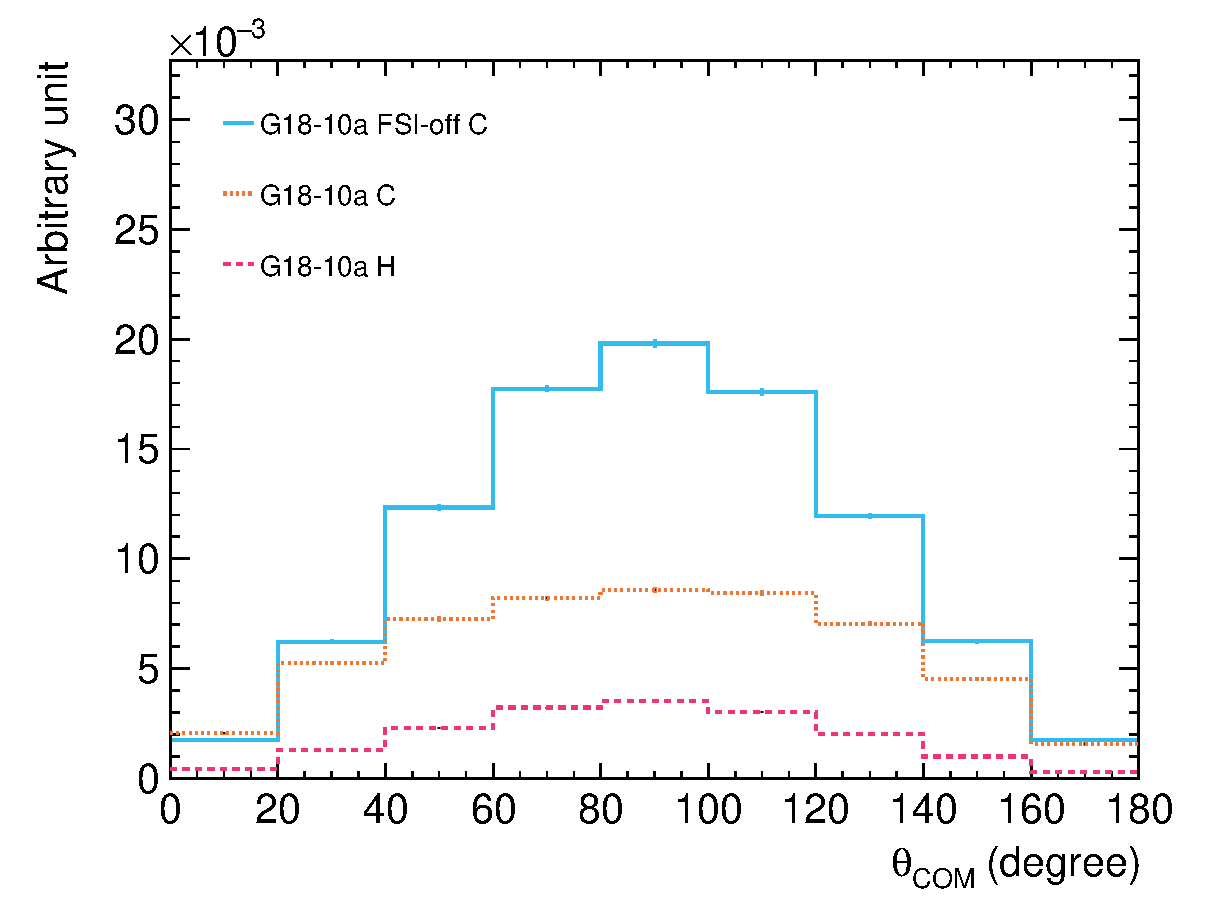
\includegraphics[width=\textwidth]{figures/COM/xnorm-CH-lfgdef_da_tan.eps} \\
          \caption{Cross-section normalized $\thetacom$ distribution - $\numuccopiop$ selection.}
          \label{subfig:ch-comp-xnorm}
     \end{subfigure}
     \begin{subfigure}[ht!]{\trfigwid\textwidth}
          \centering
          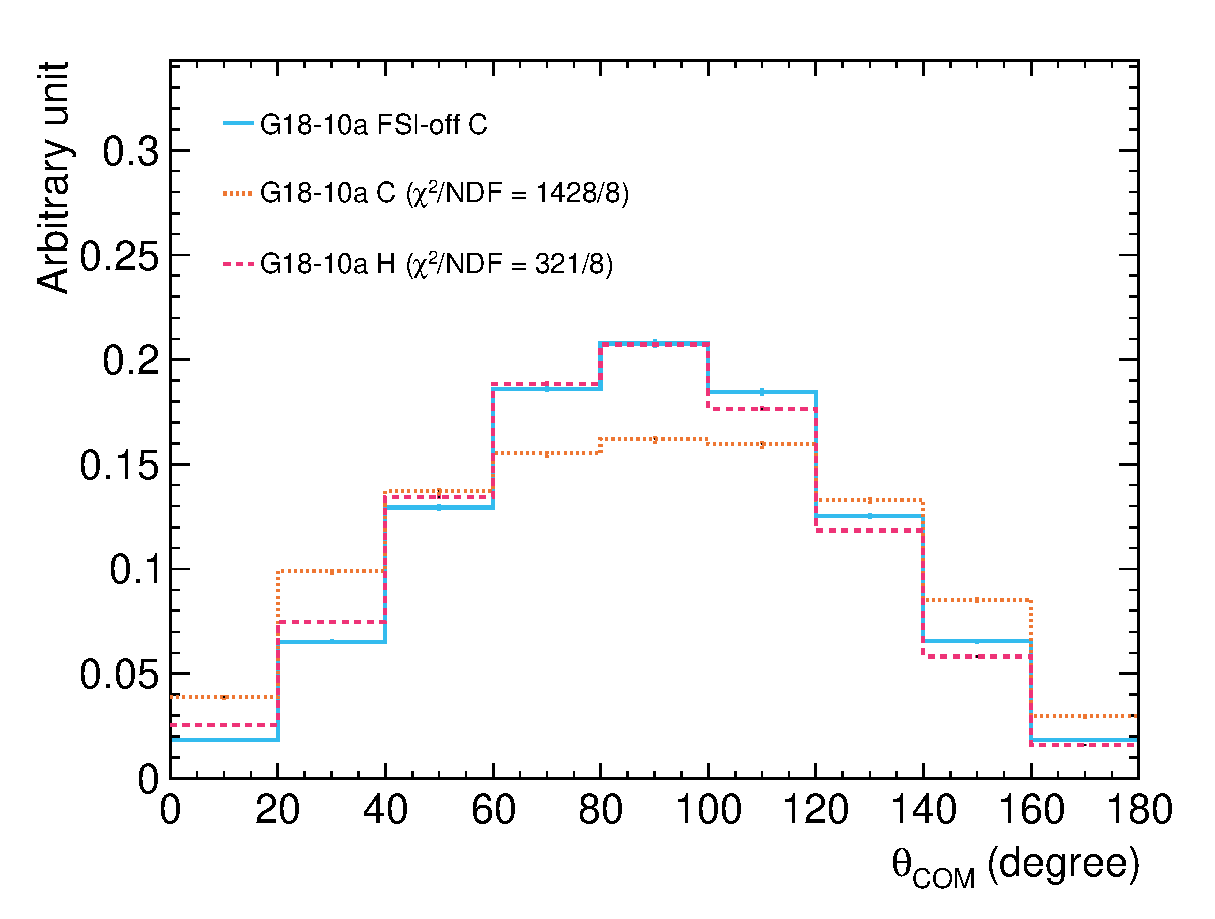
\includegraphics[width=\textwidth]{figures/COM/anorm-CH-lfgdef_da_tan.eps}     
          \caption{Area normalized $\thetacom$ distribution - $\numuccopiop$ selection.}
          \label{subfig:ch-comp-com-cc1pi1p}
     \end{subfigure}
     \begin{subfigure}[ht!]{\trfigwid\textwidth}
          \centering
          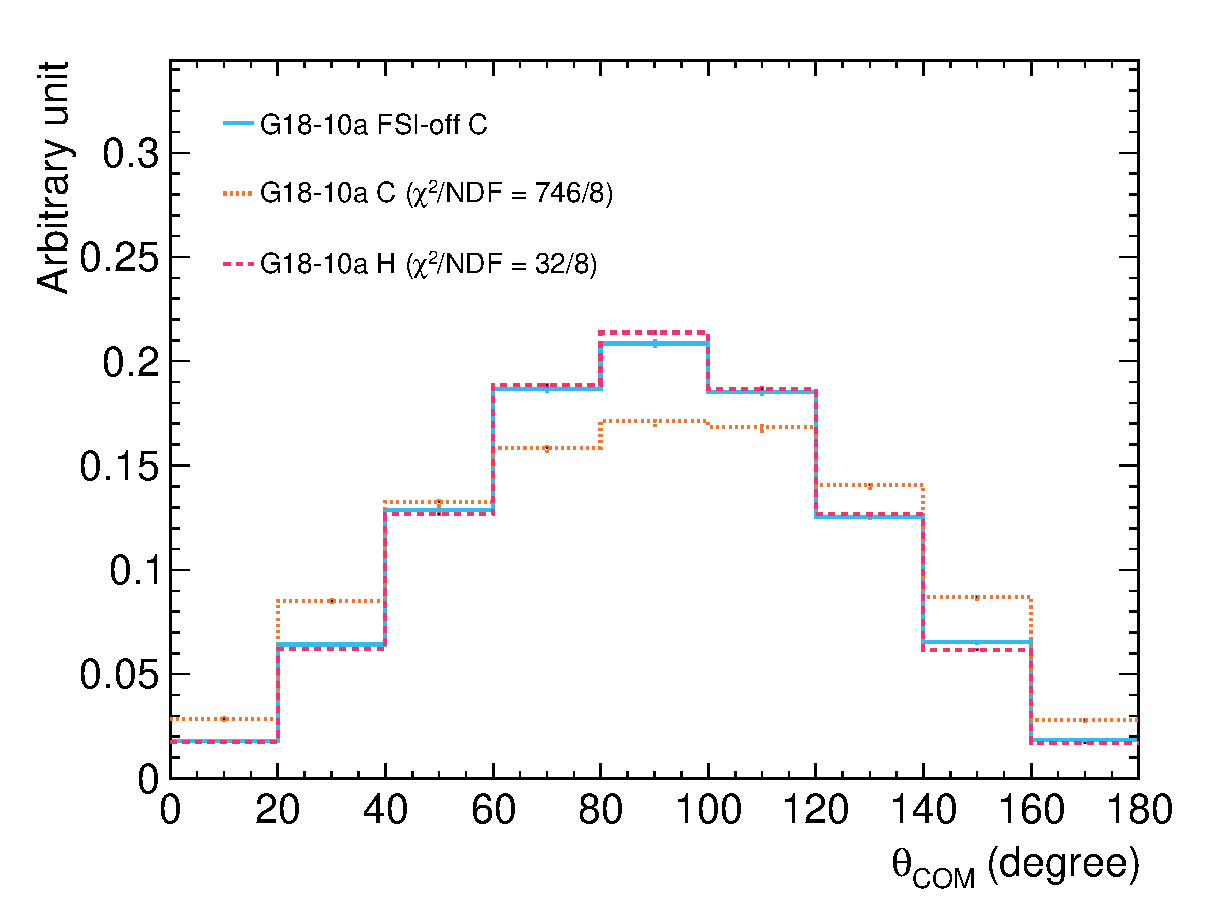
\includegraphics[width=\textwidth]{figures/COM/anorm-CH-lfgdef-resonly_da_tan.eps}  
          \caption{Area normalized $\thetacom$ distribution - $\numuccopiop$ selection restricted to $\deltapp$ decay only.}
          \label{subfig:ch-comp-com-dpp}
     \end{subfigure}
     \caption{Cross-section normalized (\ref{subfig:ch-comp-xnorm}) and area normalized (\ref{subfig:ch-comp-com-cc1pi1p} and \ref{subfig:ch-comp-com-dpp}) comparisons for FSI on/off for carbon and hydrogen with \geta for $\thetacom$ using the T2K flux. (\ref{subfig:ch-comp-com-dpp}) has a more stringent selection to restrict the resonance to be $\deltapp$.}
     \label{fig:ch-comp}
     \end{figure}

     As illustrated in Fig.~\ref{subfig:ch-comp-xnorm}, enabling or disabling FSI has a significant effect on the $\thetacom$ cross-section.
     The $\thetacom$ distributions of the two $\nu$-C (FSI-on and FSI-off) samples are considerably larger than that of $\nu$-H, owing to the larger number of nucleons.
     Given that the event selection is based on the topology (i.e. $\numuccopiop$), enabling FSI can lead to a considerable decrease in the cross section via pion absorption and via pion‐induced pion production.
     Pion charge exchange can also convert $\pip$ to $\piz$, thereby reducing the cross section; however, this type of FSI has a negligible impact for the T2K flux~\cite{GENIE:2024ufm}.
     Readers can refer to the literature (e.g. Ref.~\cite{Filali:2024vpy}) for further demonstration of the impact of FSI on the cross section.

     To examine the detailed effect of IS on $\thetacom$, the cross-section shape of $\nu$-C events (with FSI enabled and disabled) is compared to that of $\nu$-H in Fig.~\ref{subfig:ch-comp-com-cc1pi1p}.
     To better quantify the shape differences, $\chindf$ values (where NDF stands for the number of degrees of freedom) are calculated for all shape‐comparison plots.
     Each $\chindf$ value is calculated with respect to the first curve in its respective plot, accounting only for statistical uncertainties.
     As shown by the ``\geta FSI-off C'' and ``\geta C'' curves in Fig.~\ref{subfig:ch-comp-com-cc1pi1p}, enabling FSI leads to a drastic change in the cross-section shape.
     In contrast, the $\nu$-H and $\nu$-C (FSI-off) curves are much closer to each other.
     This bolsters the claim that FSI has a much stronger impact on the $\thetacom$ distribution than do IS effects.
     Nonetheless, the FSI-off $\nu$-C distribution remains considerably different from the $\nu$-H distribution, with a large $\chindf$ value of $321/8$.
     If the comparison is restricted to events from $\deltapp$ decay only (based on true information), as shown in Fig.~\ref{subfig:ch-comp-com-dpp}, the difference between the FSI-off $\nu$-C and $\nu$-H $\thetacom$ distributions is significantly reduced, with a $\chindf$ of $32/8$, suggesting that these distributions are almost statistically compatible.
     However, the large $\chindf$ observed for $\numuccopiop$ indicates that even without FSI, using carbon instead of hydrogen as the target introduces complexities beyond a simple change in the nucleon kinematic distribution.
     It is challenging to pinpoint the exact cause of this large difference, which should be reserved for investigation in future studies.

     Because comparing FSI-off carbon with FSI-off hydrogen appears to be too aggressive a test to isolate the impact of IS modeling, a more reasonable approach is to compare different IS models while keeping other factors fixed.
     The simulation results for the default \geta and its variant using the correlated Fermi gas (CFG) model are shown in Fig.~\ref{subfig:10alfg-comp-t2k}.
     The $\chindf$ value of $18/8$ between \geta (LFG) and \geta (CFG) is indeed small, suggesting that $\thetacom$ is robust against changes in IS models.
     Since $\thetaadt$ is conceptually similar to $\thetacom$ but exhibits a larger dependence on IS, it is imperative to compare the $\thetaadt$ distributions for \geta (LFG) and \geta (CFG) as well, as shown in Fig.~\ref{subfig:10alfg-comp-t2k-adt}, to assess the impact of the IS model change.
     Unexpectedly, an even smaller difference between the two curves for $\thetaadt$ is observed in Fig.~\ref{subfig:10alfg-comp-t2k-adt} compared to Fig.~\ref{subfig:10alfg-comp-t2k}, indicating that despite its dependence on IS, changing from LFG to CFG does not distort the shape of $\thetaadt$ appreciably.
     \begin{figure}
     \centering
     \begin{subfigure}[b]{\dbfigwid\textwidth}
          \centering
          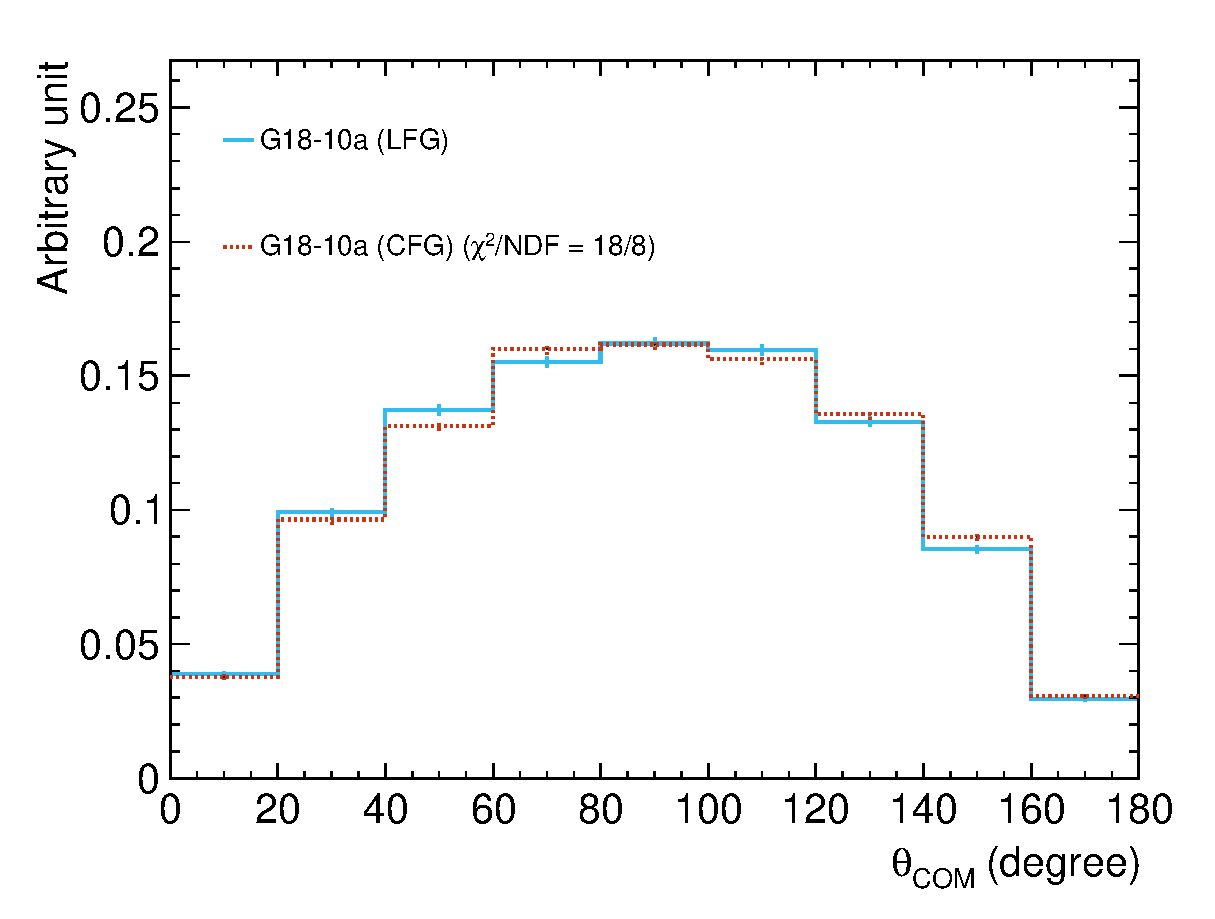
\includegraphics[width=\textwidth]{figures/COM/anorm-10a-9bin-_da_tan.eps}
          \caption{$\thetacom$}
          \label{subfig:10alfg-comp-t2k}
     \end{subfigure}
     \begin{subfigure}[b]{\dbfigwid\textwidth}
          \centering
          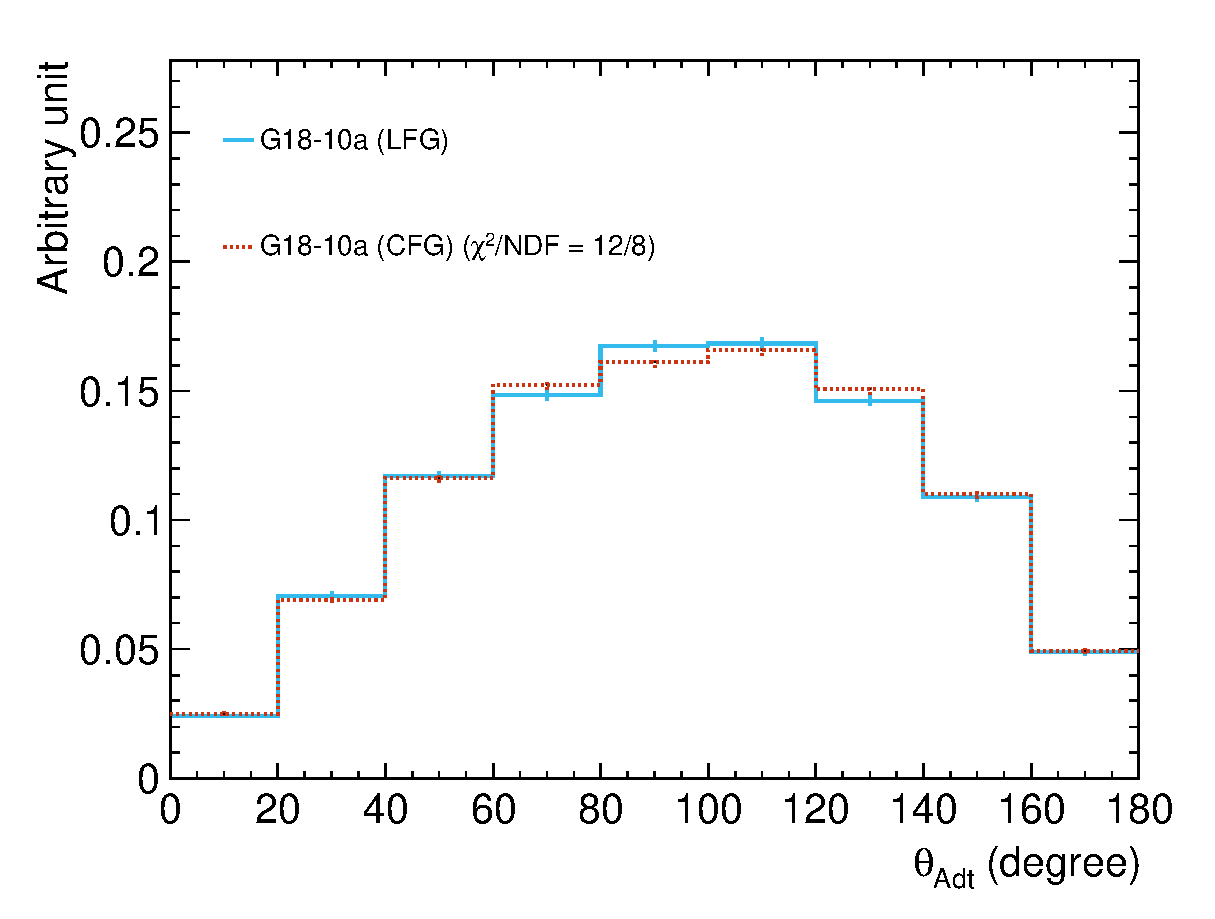
\includegraphics[width=\textwidth]{figures/COM/anorm-10a-9bin-_adt.eps}
          \caption{$\thetaadt$}
          \label{subfig:10alfg-comp-t2k-adt}
     \end{subfigure}
     \caption{Area normalized distributions for different IS models, LFG (default) and CFG, with the T2K flux on carbon. The nominal flux is \geta.}
     \label{fig:10a-comp-t2k}
     \end{figure}

     This observation could challenge the claimed IS insensitivity of $\thetacom$, as the agreement shown in Fig.~\ref{subfig:10alfg-comp-t2k} might be due to the relatively minor influence of IS.
     A further stress test was conducted by varying the removal energy of carbon across a wide range—even to unphysical levels—to assess its effect on the shapes of $\thetacom$ and $\thetaadt$.
     In \genie, the removal energy is a parameter that describes the energy required to liberate a nucleon from the nucleus.
     For a given incoming neutrino, a higher removal energy results in less of the energy transferred to the nuclear reaching the final state hadronic system.
     The results of this comparison are presented in Fig.~\ref{fig:ermc-comp}.
     \begin{figure}[ht!]
     \centering
     \begin{subfigure}[ht!]{\dbfigwid\textwidth}
          \centering
          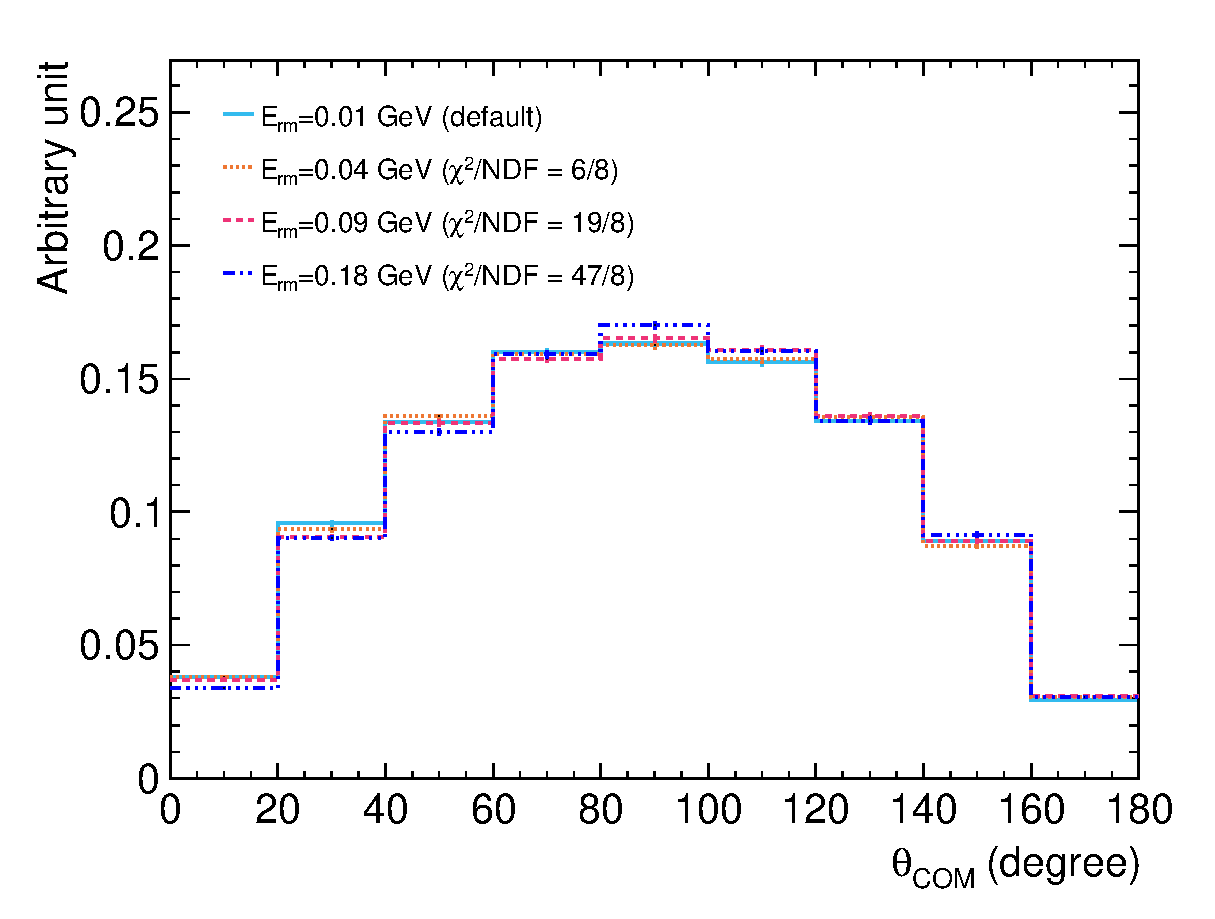
\includegraphics[width=\textwidth]{figures/COM/anorm-nuc_da_tan.eps}\\
          \caption{$\thetacom$}
          \label{subfig:ermc-comp-com}
     \end{subfigure}
     \begin{subfigure}[ht!]{\dbfigwid\textwidth}
          \centering
          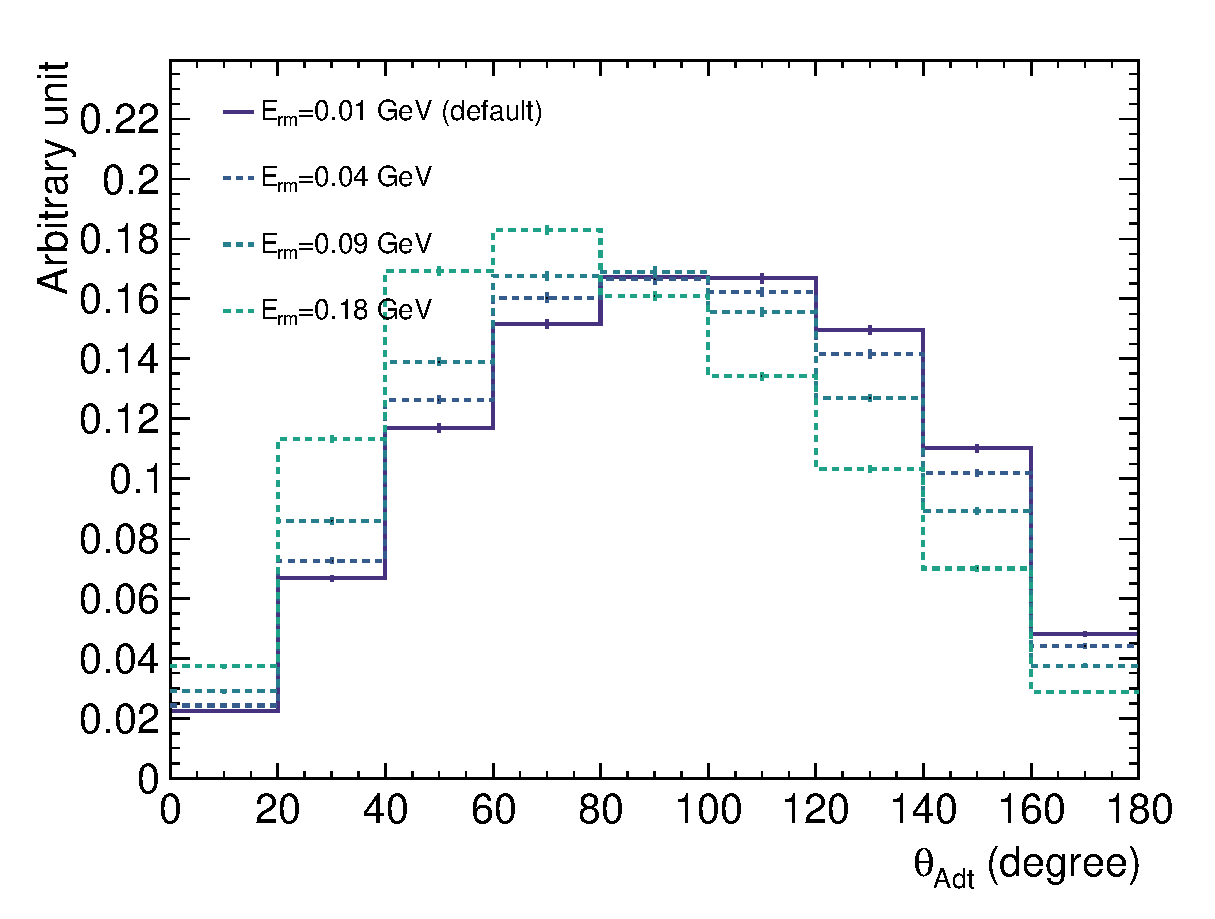
\includegraphics[width=\textwidth]{figures/COM/anorm-nuc_adt.eps}
          \caption{$\thetaadt$}
          \label{subfig:ermc-comp-adt}
     \end{subfigure}
     \caption{Area normalized comparisons for different removal energies, $E_{\textrm{rm}}$, with the T2K flux on carbon. The nominal tune is \gZero.}
     \label{fig:ermc-comp}
     \end{figure}
     As shown in Fig.~\ref{subfig:ermc-comp-com}, variations in the removal energy ($E_{\textrm{rm}}$) have very limited impact on $\thetacom$. 
     The $\thetacom$ distribution remains statistically compatible with the default removal energy of $10~\mev$, even when $E_{\textrm{rm}}$ is increased to $90~\mev$.
     When $E_{\textrm{rm}}$ is further increased to $180~\mev$, the $\thetacom$ distribution begins to deviate from the default case, although the $\chindf$ remains relatively small at $47/8$.
     In contrast, the $\thetaadt$ peak exhibits a noticeable shift accompanied by a gradual change in its shape as $E_{\textrm{rm}}$ varies.
     For $\thetaadt$, the $\chindf$ rises to $109/8$ when $E_{\textrm{rm}}$ is increased to $40~\mev$—a deviation much larger than that observed for $\thetacom$—and further increases to $3695/8$ when $E_{\textrm{rm}}$ is raised to $180~\mev$, which is unphysically high.
     These results confirm that $\thetacom$ is robust against IS effects to a large extent, whereas $\thetaadt$ is more susceptible, as predicted.
     With the strong robustness of $\thetacom$ against IS effects demonstrated relative to $\thetaadt$, the subsequent investigation will focus solely on $\thetacom$.

     Another important property of $\thetacom$ to verify is its sensitivity to FSI effects.
     Similar to the investigation of IS effects, the $\thetacom$ distributions for different FSI models are shown in Fig.~\ref{fig:fsi-comp}.
     There are two commonly used FSI models in \genie, namely hA and hN.
     Thus, two \genie tunes—\geta (hA) and \getb (hN), which differ only in FSI modeling—are compared in Fig.~\ref{subfig:10a10b-comp-t2k}.
     The $\thetacom$ distributions for these two tunes are statistically incompatible, with a large $\chindf$ value of $64/8$, a difference that is significantly more pronounced than the fluctuation induced by changing the IS model from LFG to CFG, as shown in Fig.~\ref{subfig:10alfg-comp-t2k}.
     To further verify the sensitivity of $\thetacom$ to FSI effects, a comparison between \gZero (hA) and \gC (tuned hA) is presented in Fig.~\ref{subfig:g240c-comp-t2k}.
     In \gC~\cite{GENIE:2024ufm}, the hA model has been tuned to maintain good agreement with the T2K TKI $\numuccopiop$ data~\cite{T2K:2021naz}, so the considerable difference—$\chindf=29/8$—between the two distributions in Fig.~\ref{subfig:g240c-comp-t2k} further demonstrates the sensitivity of $\thetacom$ to FSI effects.

     \begin{figure}
     \begin{subfigure}[b]{\dbfigwid\textwidth}
          \centering
          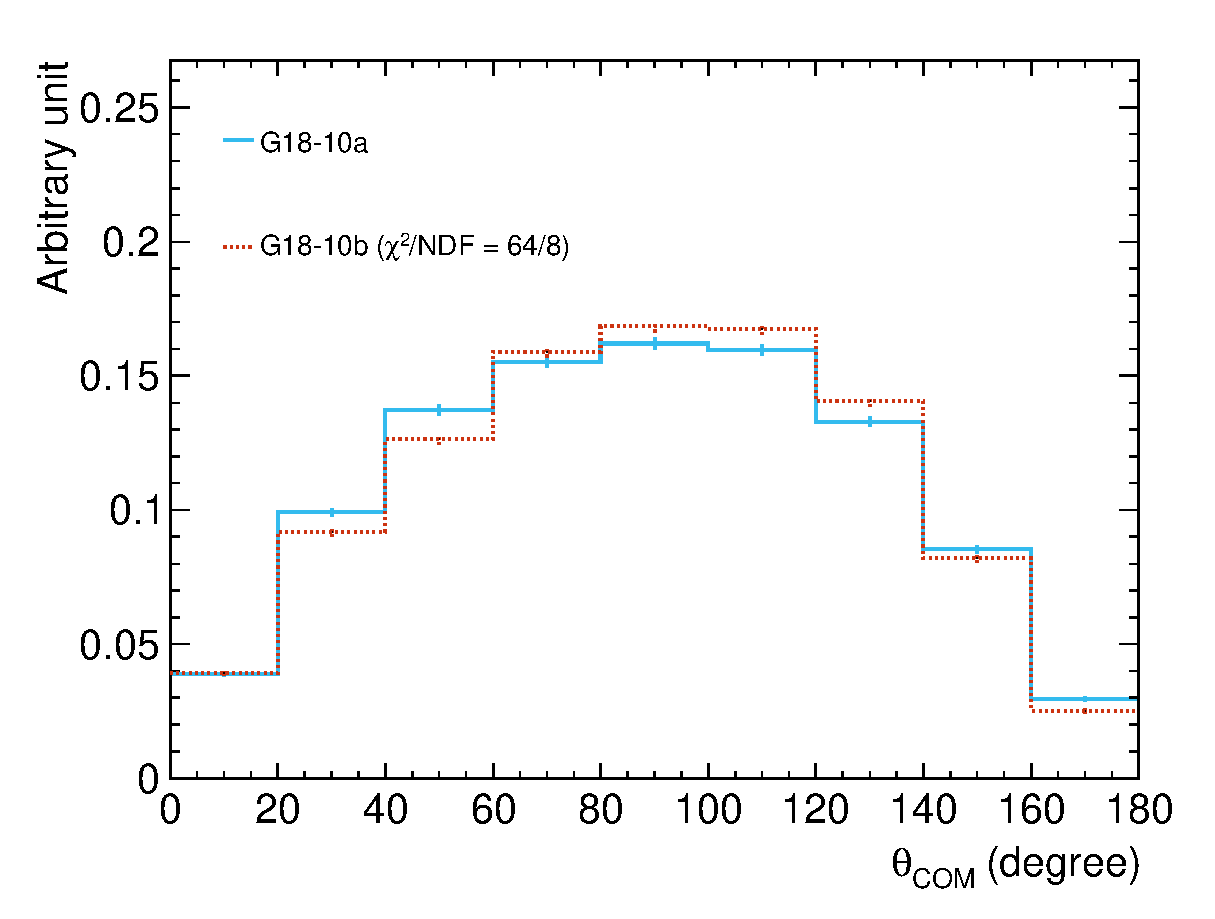
\includegraphics[width=\textwidth]{figures/COM/anorm-10a10b-lfgdef_da_tan.eps}
          \caption{\geta vs \getb }
          \label{subfig:10a10b-comp-t2k}
     \end{subfigure}
     \begin{subfigure}[b]{\dbfigwid\textwidth}
          \centering
          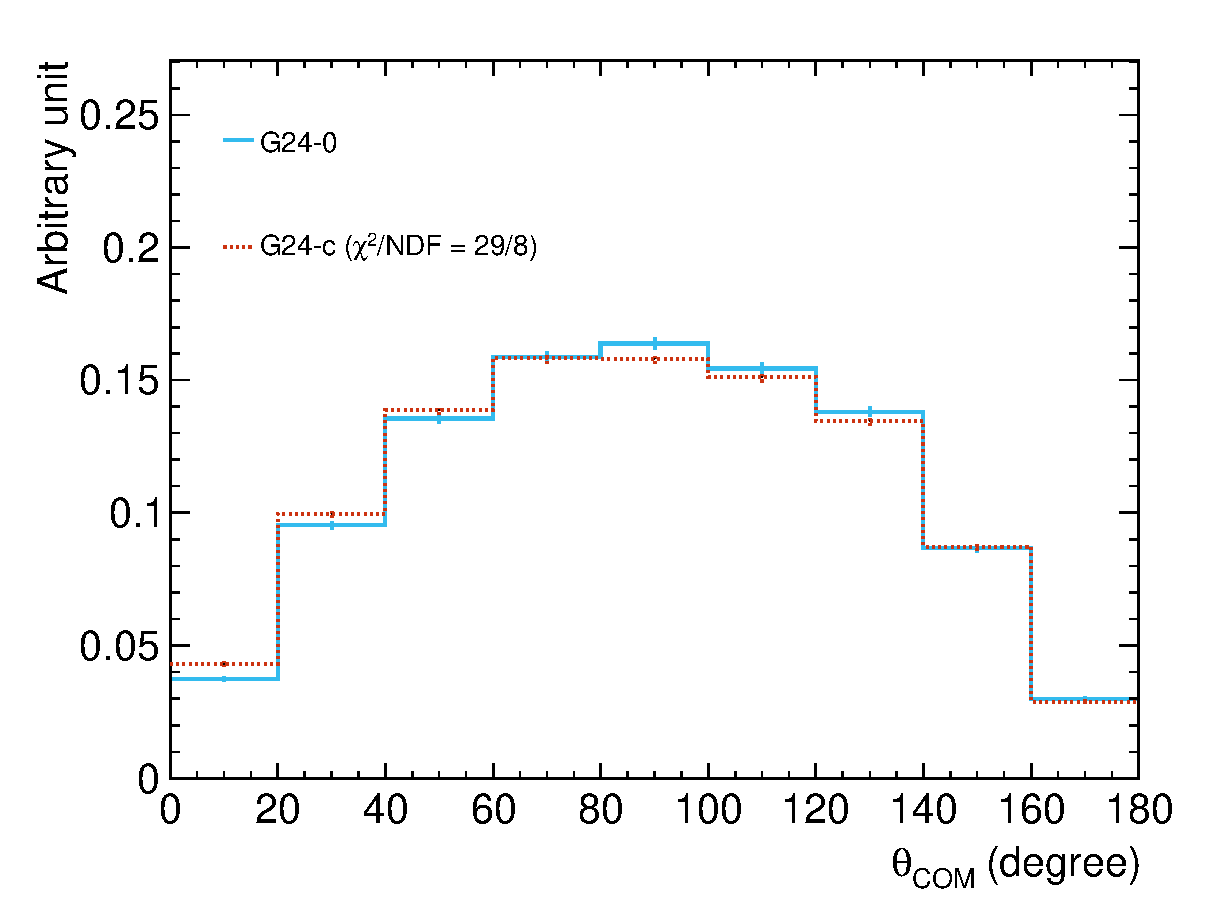
\includegraphics[width=\textwidth]{figures/COM/anorm-g240c-t2k-_da_tan.eps}
          \caption{\gZero vs \gC}
          \label{subfig:g240c-comp-t2k}
     \end{subfigure}
     \caption{Area normalized comparisons for different FSI models, \ref{subfig:10a10b-comp-t2k} for \geta (hA) and \getb (hN) and \ref{subfig:g240c-comp-t2k} for \gZero (hA) and \gC (tuned hA) with the T2K flux on carbon.}
     \label{fig:fsi-comp}
     \end{figure}

     The two major advantages of $\thetacom$ have been demonstrated, namely its robustness against IS effects and its sensitivity to FSI effects.
     The next step is to investigate the impact of other factors in neutrino–nucleus interactions on $\thetacom$.
     Since $\thetacom$ is calculated from the decay products of resonances, it can be affected by changes in RES modeling, which dictate the production and decay of these resonances.
     As a proxy for investigating the effect of a change in the RES model on $\thetacom$, the axial mass parameter, $\MA$, in the \gZero tune was varied to an exaggerated—and most likely unphysical—extent, as shown in Fig.~\ref{fig:ma-comp}.
     As anticipated, Fig.~\ref{subfig:ma-comp-xsec} demonstrates that varying $\MA$ alters the cross-section, while the shape of $\thetacom$ remains almost unchanged—as confirmed by the small $\chindf$ values in Fig.~\ref{subfig:ma-comp-area}.
     This is likely because $\deltapp$ is the dominant resonance for the T2K flux, and changes in $\MA$ do not appreciably alter its decay properties—thereby leaving the $\thetacom$ distribution largely unaffected.
     \begin{figure}
     \centering
     \begin{subfigure}[b]{\dbfigwid\textwidth}
          \centering
          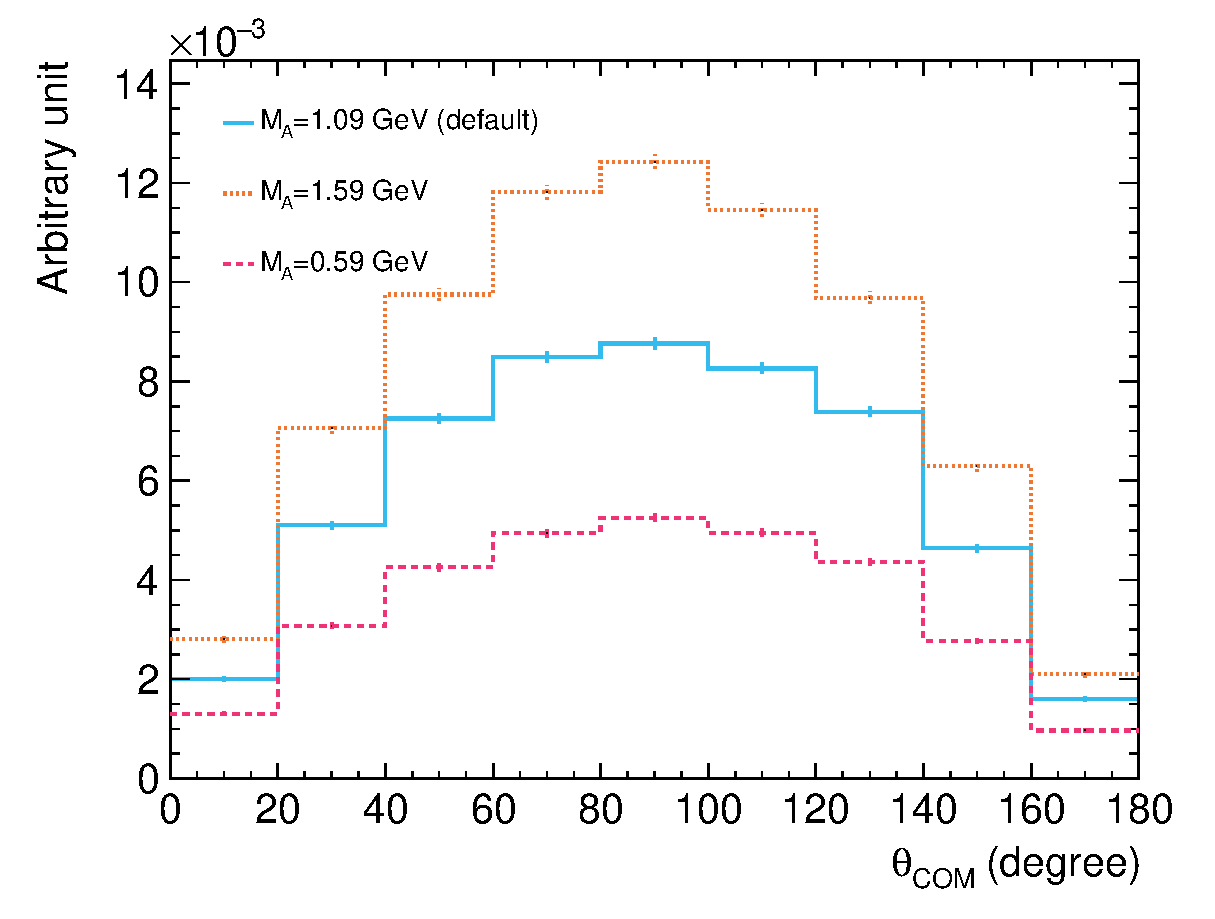
\includegraphics[width=\textwidth]{figures/COM/xnorm-ma-t2k-_da_tan.eps}
          \caption{Cross-section normalized}
          \label{subfig:ma-comp-xsec}
     \end{subfigure}
     \begin{subfigure}[b]{\dbfigwid\textwidth}
          \centering
          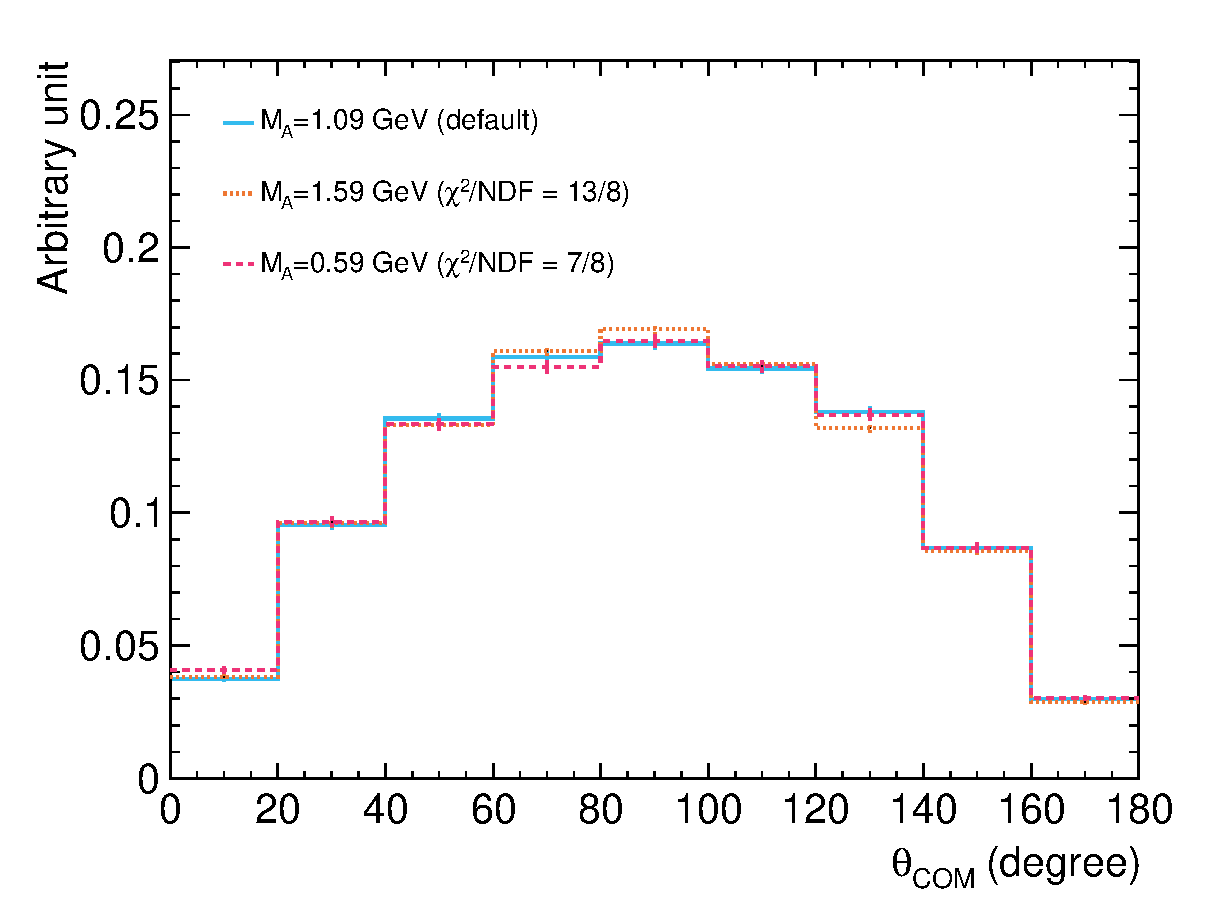
\includegraphics[width=\textwidth]{figures/COM/anorm-ma-t2k-_da_tan.eps}
          \caption{Area normalized}
          \label{subfig:ma-comp-area}
     \end{subfigure}
     \caption{Comparisons for different $\MA$ values with the T2K flux on carbon. The nominal tune is \gZero.}
     \label{fig:ma-comp}
     \end{figure}

     To complement this investigation, a similar comparison conducted using the MINERvA flux on the MINERvA target is shown in Fig.~\ref{fig:ma-comp-minerva}. 
     Since the MINERvA flux is more energetic, higher resonances also make a significant contribution.
     Changes in $\MA$ can affect the resonances differently, as demonstrated by the $W$ distribution, which represents the invariant mass of the pion-nucleon system estimated from leptonic kinematics. 
     The derivation of $W$ is readily available in the literature, such as in Ref.~\cite{Paschos:2003qr}.
     As evident in Fig.~\ref{subfig:ma-comp-minerva-w}, when $\MA$ decreases to $0.59~\gev$, the relative contribution of resonances above $1.8~\gev$ increases, while the contribution of those below decreases appreciably.
     In contrast, when $\MA$ increases to $1.59~\gev$, the relative contribution of resonances above $1.8~\gev$ decreases, while the contribution of those below either increases or remains relatively unchanged.
     Consequently, these changes in $\MA$ lead to considerable differences in the $\thetacom$ distributions, with $\chindf=28/8$ for $\MA=1.59~\gev$ and $\chindf=44/8$ for $\MA=0.59~\gev$, as shown in Fig.~\ref{subfig:ma-comp-minerva}.
     To minimize the influence of higher resonances, a practical cut, $\ecom<1330~\mev$, aimed at selecting $\deltapp$ events, is imposed on the selection in Fig.~\ref{subfig:ma-comp-minerva-wcut}.
     As anticipated, the higher resonances in the $W$ distribution have largely disappeared in Fig.~\ref{subfig:ma-comp-minerva-wcut-w}, and the $\thetacom$ distributions for different $\MA$ values in Fig.~\ref{subfig:ma-comp-minerva} become statistically compatible.
     This suggests that for an energetic flux such as the MINERvA flux—which produces multiple resonances—the $\thetacom$ distribution can still be used to study FSI with minimal impact from RES modeling by imposing an $\ecom$ cut to select only $\deltapp$ events.
     \begin{figure}
     \centering
     \begin{subfigure}[b]{\dbfigwid\textwidth}
          \centering
          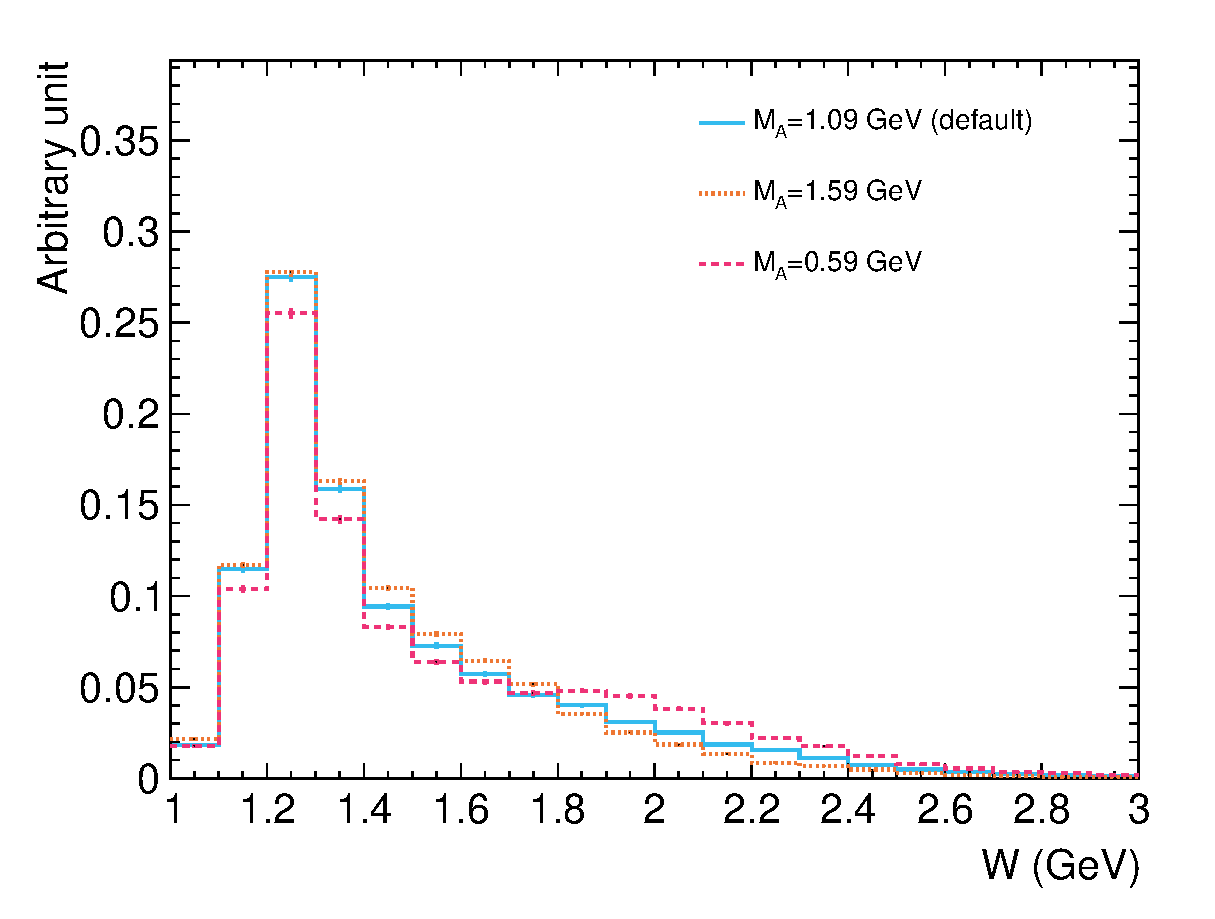
\includegraphics[width=\textwidth]{figures/COM/anorm-ma-minerva-600k-_wnucrest.eps}
          \caption{$\numuccopiop$}
          \label{subfig:ma-comp-minerva-w}
     \end{subfigure}
     \begin{subfigure}[b]{\dbfigwid\textwidth}
          \centering
          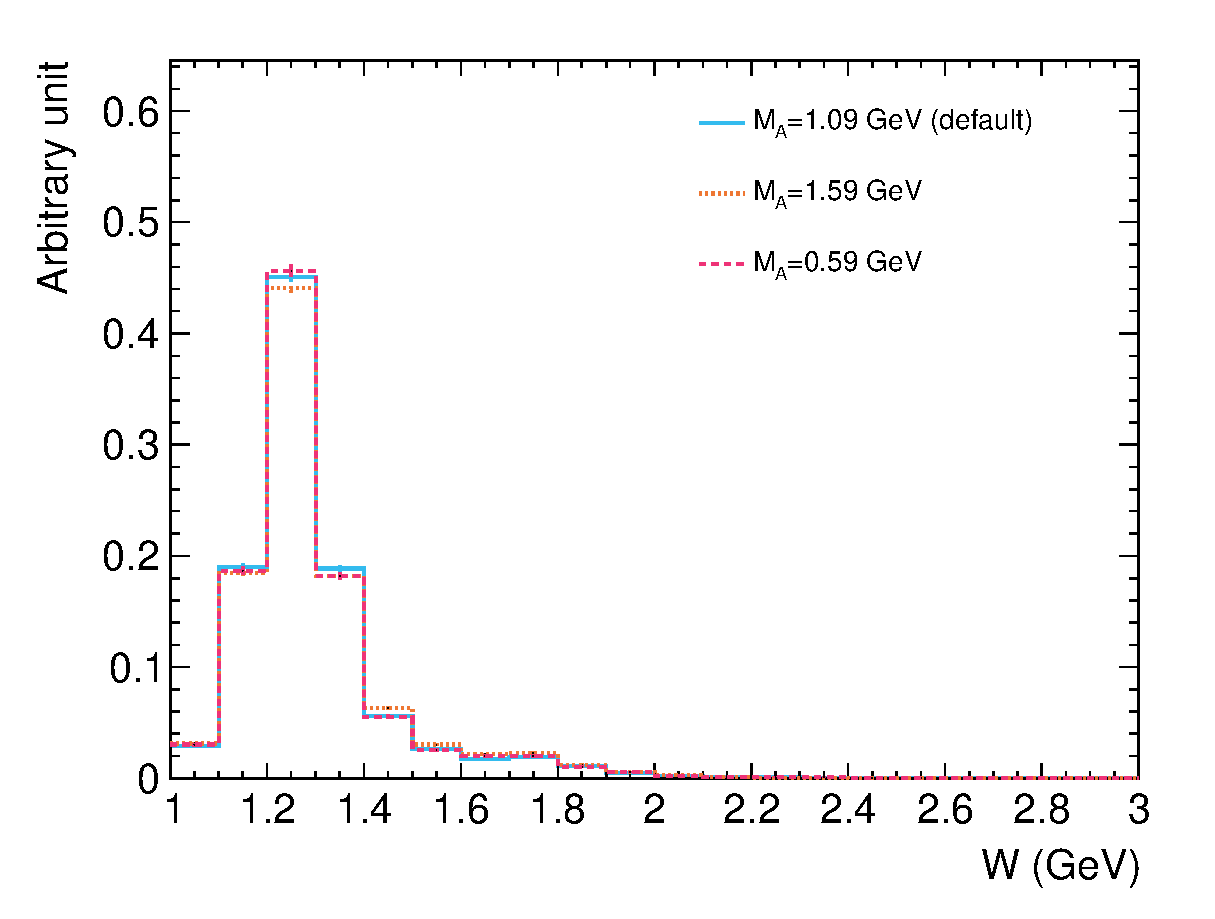
\includegraphics[width=\textwidth]{figures/COM/anorm-ma-minerva-600k-wcut_wnucrest.eps}
          \caption{$\numuccopiop$ with $\ecom<1330~\mev$}
          \label{subfig:ma-comp-minerva-wcut-w}
     \end{subfigure}
     \\
     \begin{subfigure}[b]{\dbfigwid\textwidth}
          \centering
          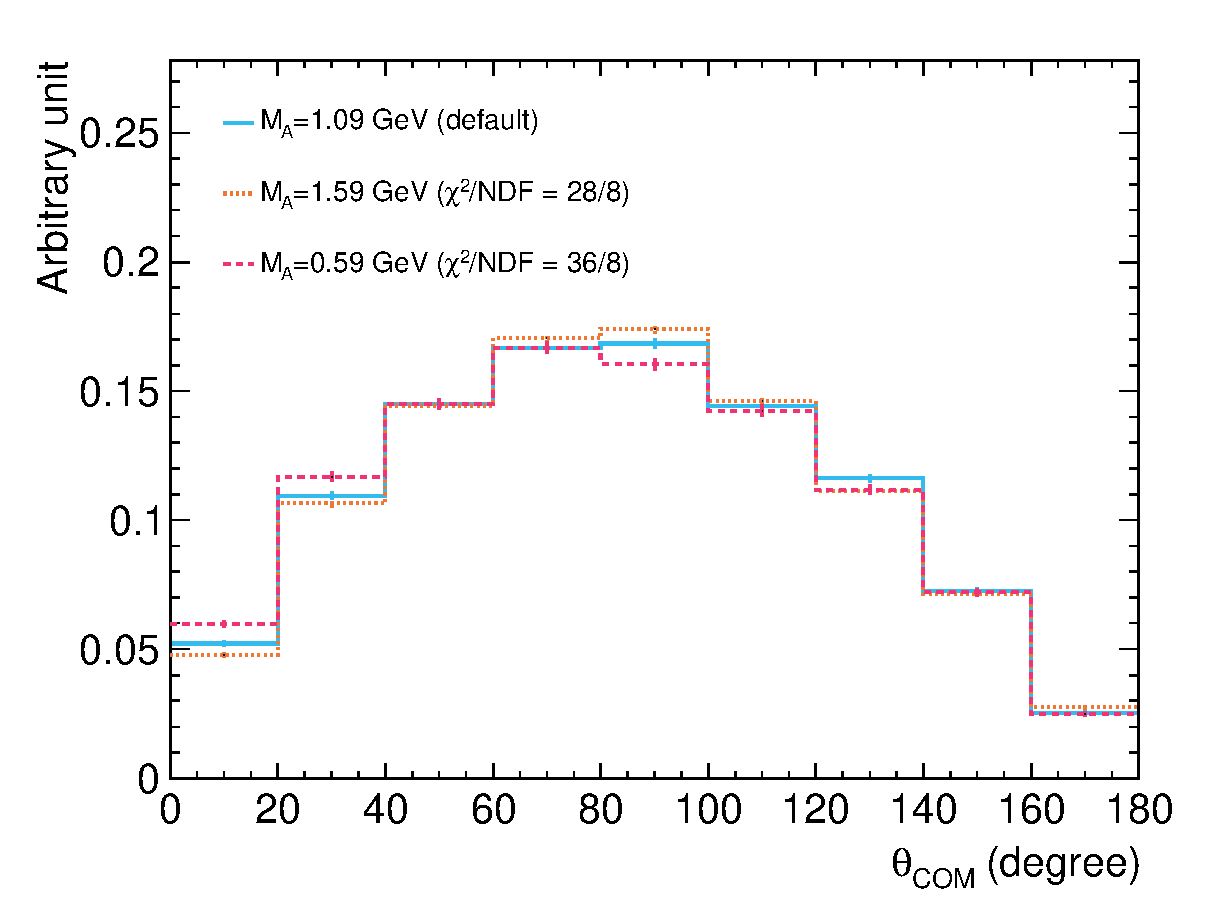
\includegraphics[width=\textwidth]{figures/COM/anorm-ma-minerva-600k-_da_tan.eps}
          \caption{$\numuccopiop$}
          \label{subfig:ma-comp-minerva}
     \end{subfigure}
     \begin{subfigure}[b]{\dbfigwid\textwidth}
          \centering
          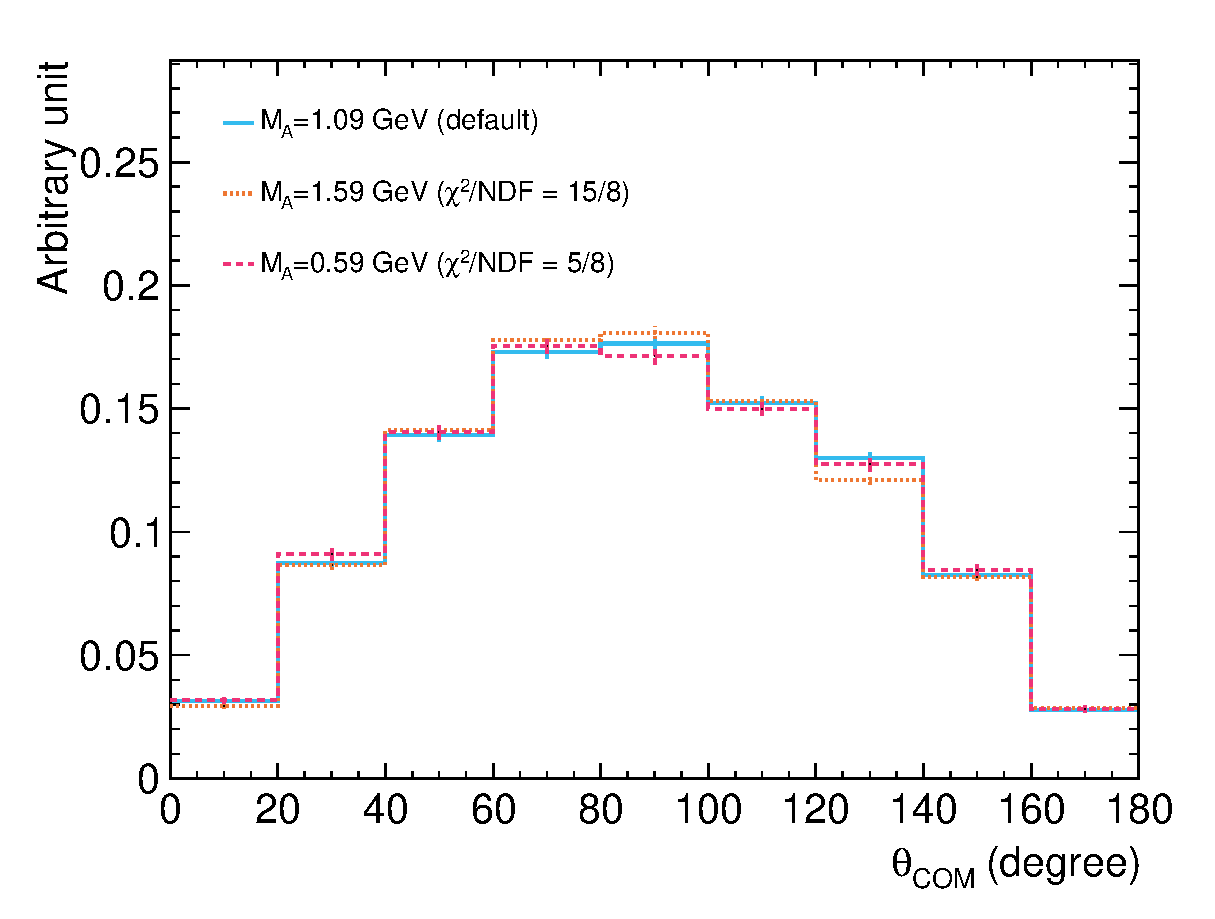
\includegraphics[width=\textwidth]{figures/COM/anorm-ma-minerva-600k-wcut_da_tan.eps}
          \caption{$\numuccopiop$ with $\ecom<1330~\mev$}
          \label{subfig:ma-comp-minerva-wcut}
     \end{subfigure}
     \caption{Area normalized comparisons of $W$ and $\thetacom$ for different $\MA$ values with the MINERvA flux on the MINERvA target. The nominal tune is \gZero.}
     \label{fig:ma-comp-minerva}
     \end{figure}

     Besides varying a parameter in the RES model, a more aggressive test is to compare two different RES models directly.
     This comparison is achieved by contrasting two \genie tunes—\geoa (employing the RS model) and \getwoa (employing the BS model)—as shown in Fig.~\ref{fig:0102a-comp}.
     The results using the T2K flux and the MINERvA flux are presented in Fig.~\ref{subfig:0102a-comp-t2k} and Fig.~\ref{subfig:0102a-comp-minerva}, respectively.
     Both $\chindf$ values are low—specifically, $6/8$ and $8/8$—suggesting that this change in the RES model is far less extreme than the unphysically large modification of $\MA$ shown in Fig.~\ref{fig:ma-comp} and that such a reasonable change in RES modeling does not lead to a noticeable alteration of the $\thetacom$ distribution.
     \begin{figure}
     \centering
     \begin{subfigure}[b]{\dbfigwid\textwidth}
          \centering
          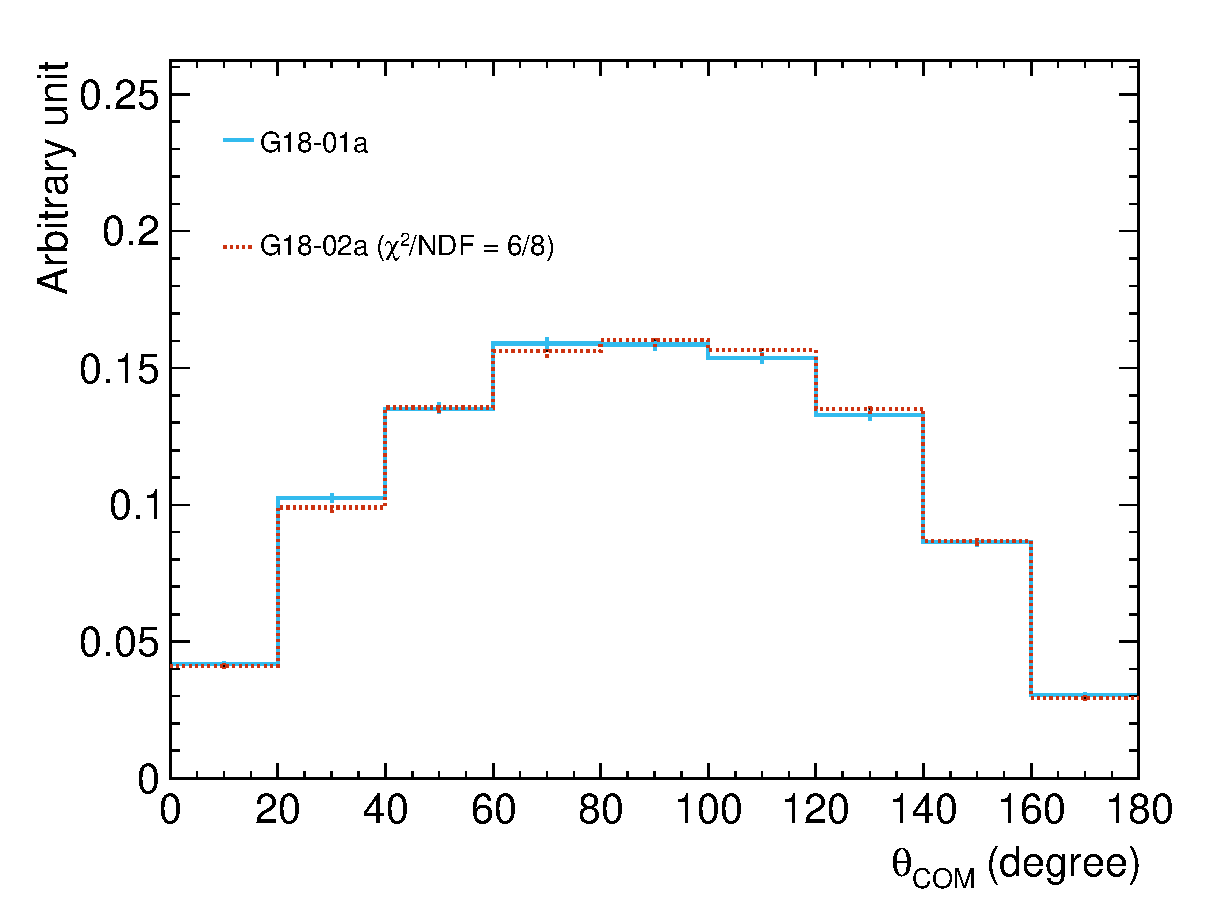
\includegraphics[width=\textwidth]{figures/COM/anorm-01a-02a_da_tan.eps}
          \caption{T2K}
          \label{subfig:0102a-comp-t2k}
     \end{subfigure}
     \begin{subfigure}[b]{\dbfigwid\textwidth}
          \centering
          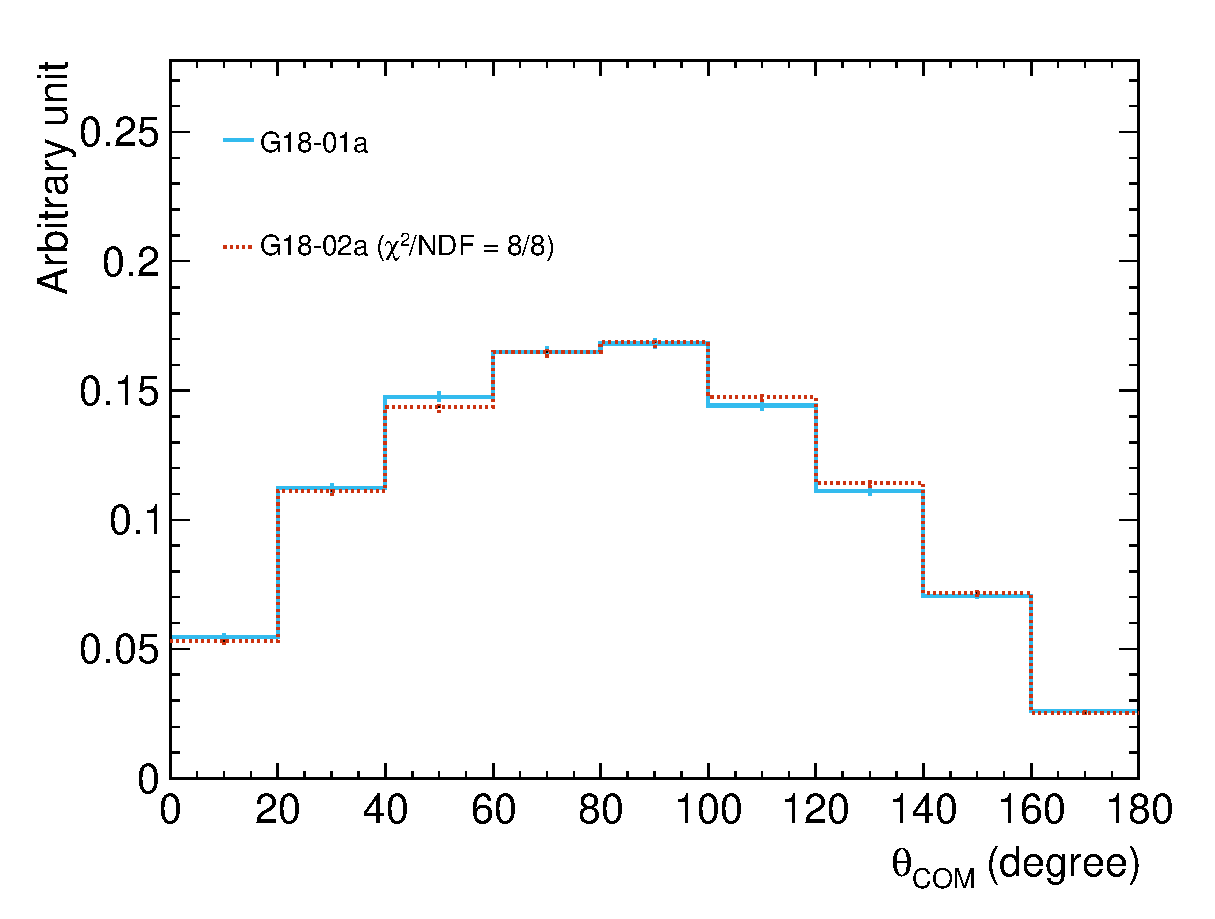
\includegraphics[width=\textwidth]{figures/COM/anorm-01a-02a-minerva_da_tan.eps}
          \caption{MINERvA}
          \label{subfig:0102a-comp-minerva}
     \end{subfigure}
     \caption{Area normalized comparisons for different RES models with the T2K (\ref{subfig:0102a-comp-t2k}) and MINERvA (\ref{subfig:0102a-comp-minerva}) fluxes using \geoa and \getwoa.
     Both select $\numuccopiop$ events, but the MINERvA sample has a additional cut of $\ecom<1330~\mev$.}
     \label{fig:0102a-comp}
     \end{figure}

     On one hand, restricting the analysis to $\deltapp$ events—by imposing an $\ecom$ cut—can minimize the impact of RES modeling on $\thetacom$ even for an energetic beam like the MINERvA flux.
     On the other hand, this behavior implies that $\thetacom$ is sensitive to the onset of higher resonances.
     Given that the robustness of $\thetacom$ against both IS effects and considerable changes of RES modeling have been demonstrated, the difference between the $\thetacom$ distributions with and without the $\ecom$ cut (as shown in Fig.~\ref{fig:ma-comp-minerva}) is most likely attributable to the onset of higher resonances.
     This advocates employing $\thetacom$ to study both the production of higher resonances and the correlations among their production.
     Since the BS model in \genie does not implement resonance correlations, this potential application of $\thetacom$ is reserved for future studies—when more advanced models, such as the MK model~\cite{Kabirnezhad:2017jmf,Kabirnezhad:2020wtp,Kabirnezhad:2022znc}, are reliably implemented and validated.

     Besides its appealing sensitivity and robustness, $\thetacom$ has the practical advantage that its reconstruction does not require determining the kinematics of the incoming neutrino.
     This decouples the reconstruction of $\thetacom$ from the systematic uncertainties associated with neutrino energy reconstruction—which are among the largest in neutrino measurements~\cite{T2K:2019yqu,T2K:2021naz,MicroBooNECollaboration:2024gvg,NOvA:2023uxq,MINERvA:2022djk}.
     However, the reconstruction of $\thetacom$ still depends on the accurate reconstruction of proton kinematics, which is itself a significant source of systematic uncertainty.
     The overall impact on precision for $\thetacom$ measurements will be investigated in future studies for specific experiments.

     To assess the impact of $\enu$ on $\thetacom$, mono-energy neutrino beams are used to simulate $\nu$-H events using tune \gZero, as shown in Fig.~\ref{fig:enu-comp-h}.
     Hydrogen is chosen as the target to isolate the impact solely due to $\enu$, while complications arising from FSI will be discussed later.
     \begin{figure}[ht!]
     \centering
     \begin{subfigure}[ht!]{\dbfigwid\textwidth}
          \centering
          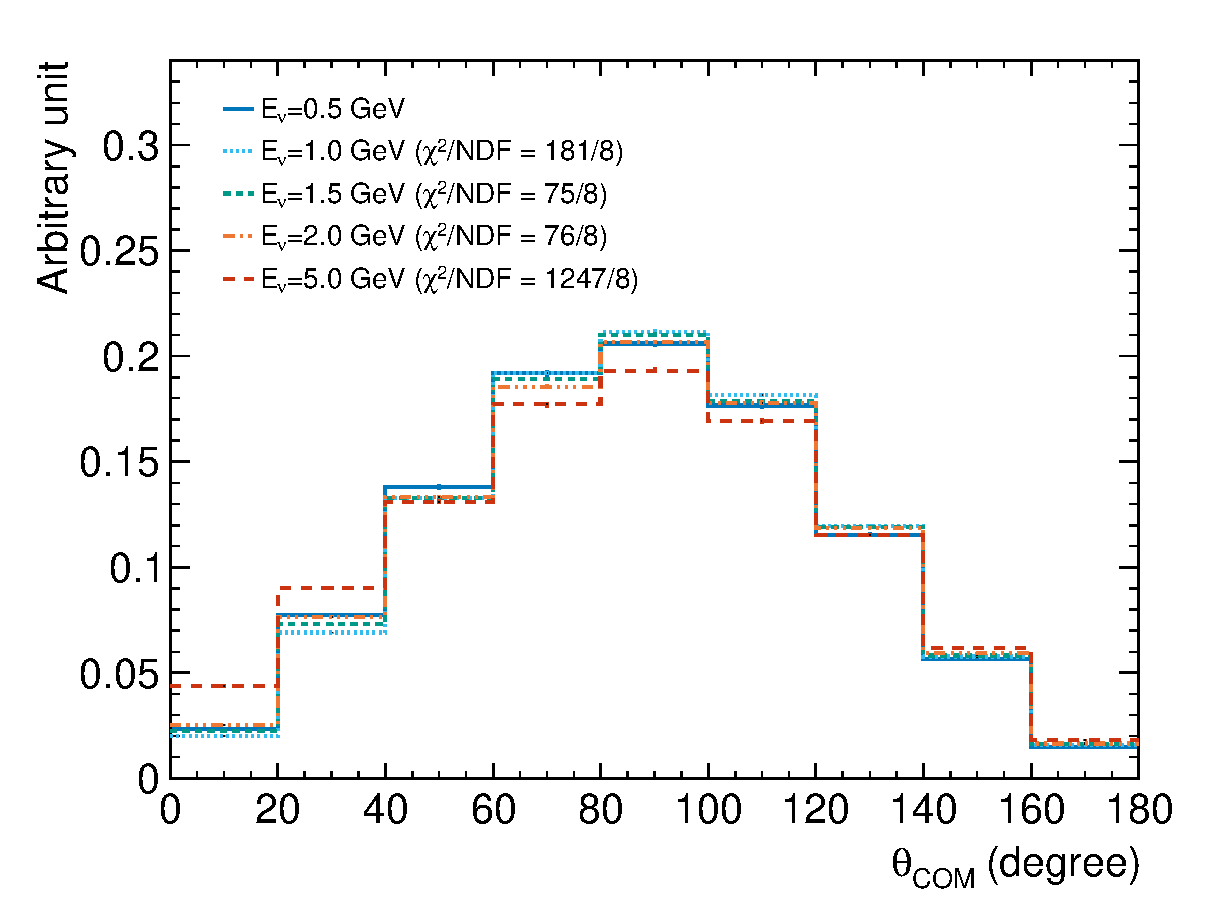
\includegraphics[width=\textwidth]{figures/COM/anorm-enu-9bin-_da_tan.eps}
          \caption{$\numuccopiop$}
          \label{subfig:enu-comp-cc1pi1p}
     \end{subfigure}
     \begin{subfigure}[ht!]{\dbfigwid\textwidth}
          \centering
          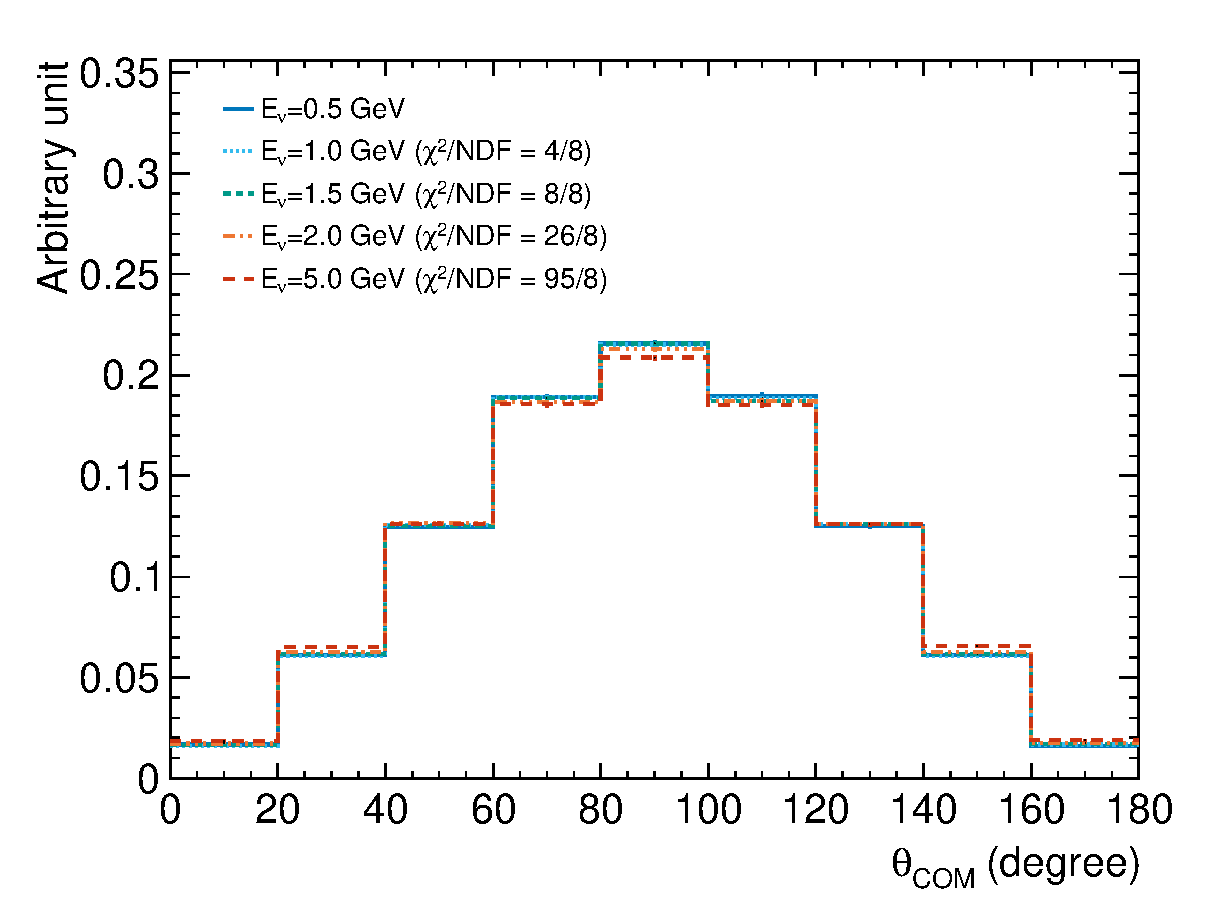
\includegraphics[width=\textwidth]{figures/COM/anorm-enu-9bin-resonly-_da_tan.eps}
          \caption{$\deltapp$ only}
          \label{subfig:enu-comp-dpp}
     \end{subfigure}
     \caption{Area normalized comparisons for different $\enu$ fluxes on hydrogen for $\thetacom$. The nominal tune is \gZero.}
     \label{fig:enu-comp-h}
     \end{figure}

     In Fig.~\ref{subfig:enu-comp-cc1pi1p}, although the shapes of the $\thetacom$ distributions appear largely consistent for $\enu$ values between $0.5~\gev$ and $2.0~\gev$, they are statistically incompatible—with $\chindf$ values on the order of $100/8$. 
     This inconsistency is likely due to the onset of higher doubly positive resonances. 
     While $\thetacom$ for a single resonance is largely independent of the production mechanism—unless a strong correlation exists between production and decay—it will be affected when the relative contributions of different resonances vary due to their distinct decay properties. 
     If the analysis is restricted to $\deltapp$ events (based on true information), as in Fig.~\ref{subfig:enu-comp-dpp}, it is encouraging to observe that all $\enu$ distributions—except for $\enu=5.0~\gev$—become compatible with much smaller $\chindf$ values, thereby confirming the independence of $\thetacom$ from $\enu$ for a single resonance.

     In the case of $\enu=5.0~\gev$, much more energetic $\deltapp$ resonances are produced, which enhance the influence of $\deltapp$ kinematics on their decay and tend to favor either very small or very large pion angles.
     Since such highly energetic neutrinos contribute only marginally to actual cross‐section measurements, this effect is not expected to pose a significant challenge for the practical application of $\thetacom$ in neutrino analyses.
     A comprehensive explanation of this observation is beyond the scope of this work; instead, a more detailed investigation of the correlation between resonance production and decay is warranted in future studies.

     In the resonance rest frame, the pion decay angle is an intrinsic property of the resonance and should be largely independent of its kinematics—and consequently, of $\enu$.
     However, in the lab frame the boost experienced by the decay products results in different hadronic kinematic distributions.
     Since FSI depends on the hadronic kinematics, the measured kinematics—and hence $\thetacom$—are indirectly affected by $\enu$.
     Therefore, although the reconstruction of $\thetacom$ for an individual event is independent of $\enu$, the overall $\thetacom$ distribution may vary due to changes in the neutrino energy spectrum when FSI is present.
     To assess this impact in practice, mono-energetic neutrino beams are used to simulate $\nu$-C events using tune \gZero, and the results are compared to those obtained with the T2K flux, as shown in Fig.~\ref{fig:enu-comp-c}.
     \begin{figure}[ht!]
     \centering
     \begin{subfigure}[ht!]{\dbfigwid\textwidth}
          \centering
          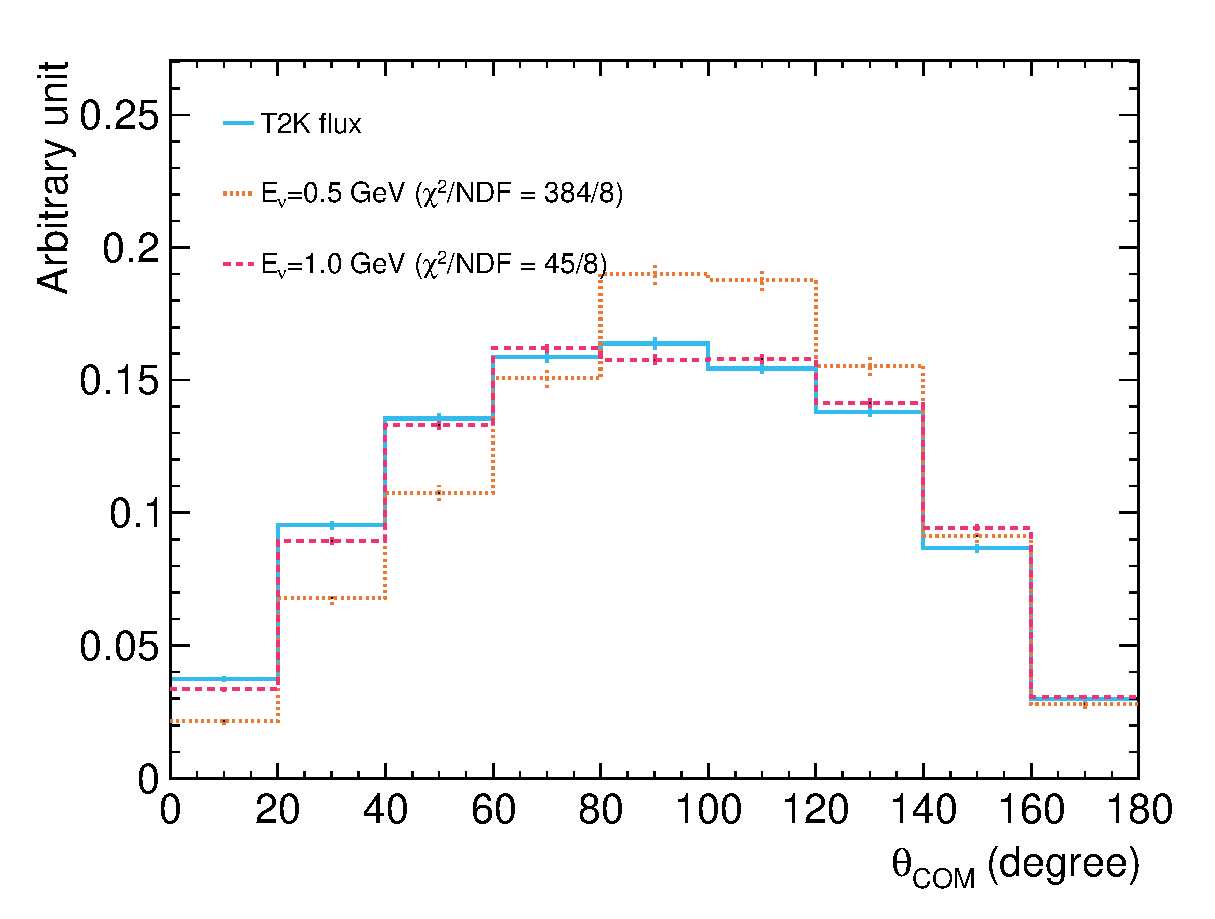
\includegraphics[width=\textwidth]{figures/COM/anorm-enu-c-9bin-_da_tan.eps}
          \caption{$\numuccopiop$}
          \label{subfig:enu-comp-cc1pi1p-c}
     \end{subfigure}
     \begin{subfigure}[ht!]{\dbfigwid\textwidth}
          \centering
          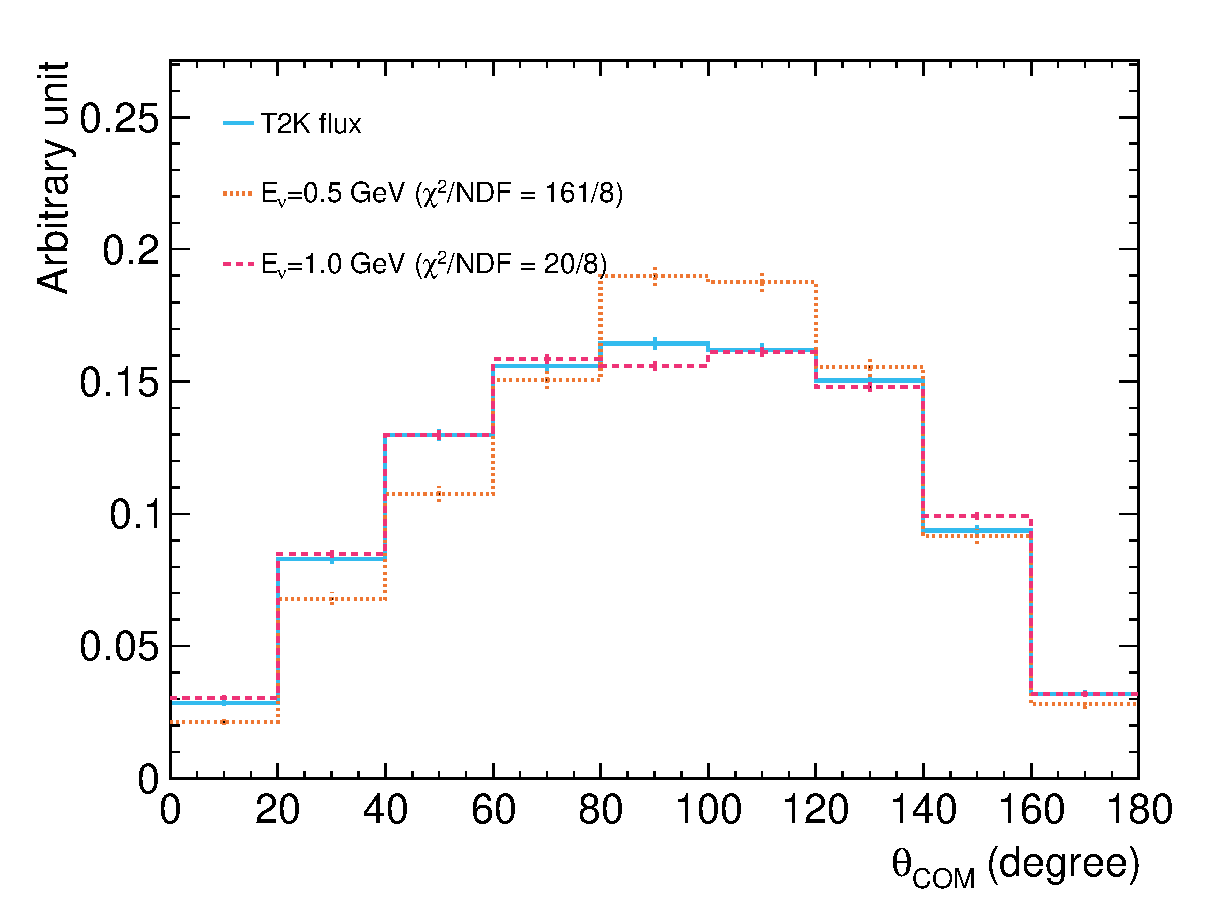
\includegraphics[width=\textwidth]{figures/COM/anorm-enu-c-9bin-wcut_da_tan.eps}
          \caption{$\numuccopiop$ with $\ecom<1330~\mev$}
          \label{subfig:enu-comp-dpp-c}
     \end{subfigure}
     \caption{Area normalized comparisons for different $\enu$ fluxes and the T2K flux on carbon for $\thetacom$. The nominal tune is \gZero.}
     \label{fig:enu-comp-c}
     \end{figure}

     As expected, variations in hadronic kinematics caused by different $\enu$ values lead to noticeable changes in the $\thetacom$ distribution, as illustrated in Fig.~\ref{subfig:enu-comp-cc1pi1p-c}.
     This effect is more pronounced for $\enu=0.5~\gev$, where low-momentum pions—the decay products of low-momentum $\deltapp$ resonances resulting from low-energy neutrinos—are more likely to be absorbed through FSI.
     Thus, even with an $\ecom < 1330~\mev$ cut imposed, the $\thetacom$ distribution for $\enu=0.5~\gev$ remains incompatible with that for the T2K flux, whereas the $\enu=1.0~\gev$ distribution becomes relatively compatible with the T2K flux, exhibiting a $\chindf$ value of $20/8$.
     This implies that even in the extreme case where the T2K neutrino energies are misestimated to be uniformly $1~\gev$, the resulting $\thetacom$ distribution would remain consistent.
     This finding strongly corroborates the practical robustness of $\thetacom$ against $\enu$ variations, provided that an $\ecom < 1330~\mev$ cut is applied for the T2K flux.
     A similar level of robustness should be attainable for other fluxes, although flux-specific cuts may be necessary; this remains an avenue for future investigation.

     The observed robustness of $\thetacom$ against $\enu$ variations in $\nu$-H events—across a wide range of $\enu$ with an $\ecom < 1330~\mev$ cut, as seen in Fig.~\ref{fig:enu-comp-h}—opens up a new avenue for cross-experiment comparisons.
     As depicted in Fig.~\ref{fig:flux-comp}, the $\thetacom$ distributions for the T2K, MINERvA, and MicroBooNE~\footnote{There is no hydrogen in the target for MicroBooNE, but such a simulation is possible and plotted for reference only.} fluxes on a hydrogen target using tune \gZero are highly statistically compatible, with $\chindf$ values of $10/8$ and $9/8$, respectively.
     \begin{figure}
     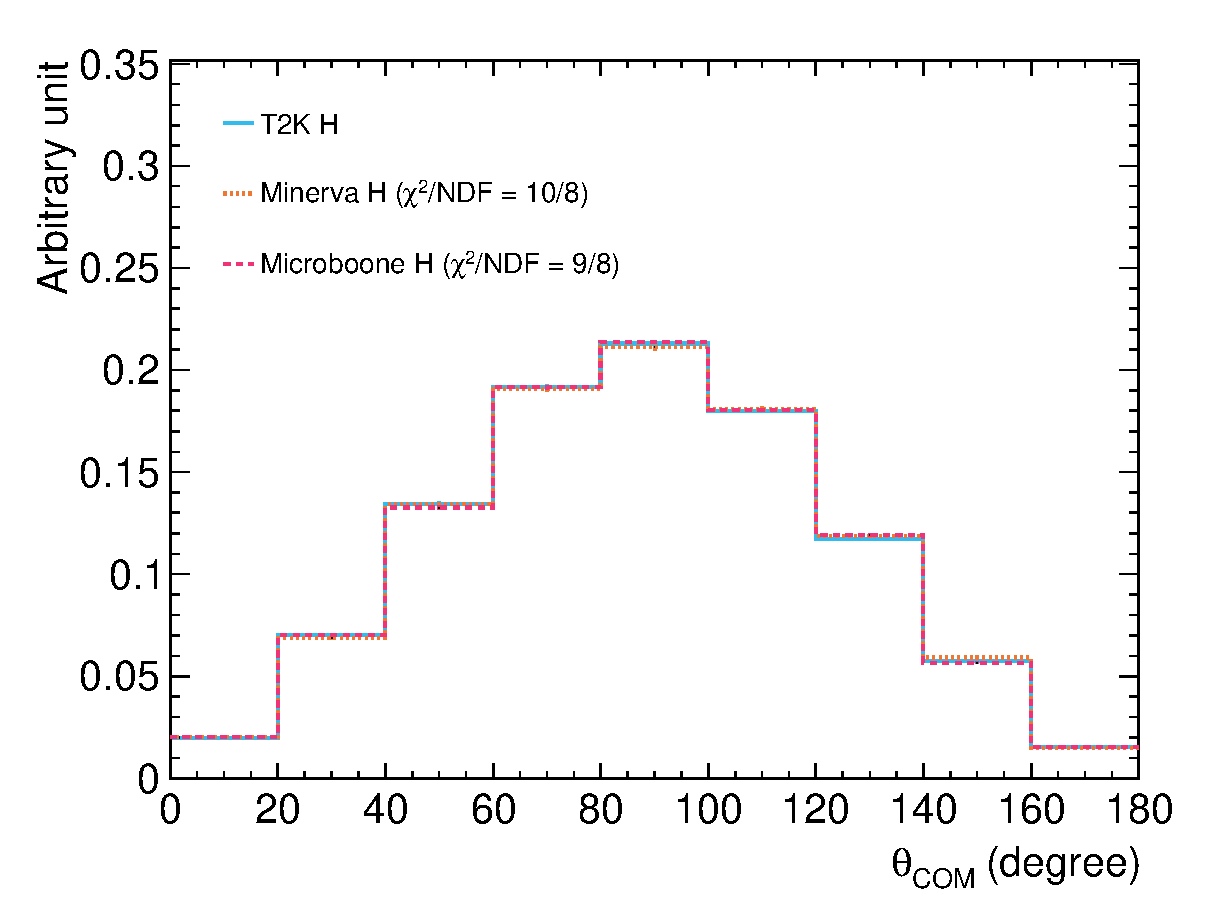
\includegraphics[width=\scfigwid\textwidth]{figures/COM/anorm-flux-9bin-wcut_da_tan.eps}
     \caption{Area normalized comparisons for different fluxes on hydrogen with the $\ecom<1330~\mev$ cut imposed for MINERvA. The nominal tune is \gZero.}
     \label{fig:flux-comp}
     \end{figure}
     The advantage of a $\nu$-H selection is that it avoids the complications introduced by FSI affecting the hadronic kinematics in the lab frame, as illustrated in Fig.~\ref{fig:enu-comp-c}.
     Consequently, despite differing energy profiles, the neutrino fluxes from these experiments yield nearly identical $\thetacom$ distribution shapes.
     In practice, MINERvA~\cite{MINERvA:2023avz} has already conducted a $\nu$-H selection, and the T2K collaboration is planning similar analyses~\cite{Lu:2015hea}, thereby demonstrating the feasibility of such cross-experiment comparisons in the future.
     Given a high‐purity hydrogen sample, the $\thetacom$ cross section can be directly compared across different experiments.

     Thus far, the discussion has primarily focused on the insensitivity of $\thetacom$ to variations in one aspect (excluding FSI) of the complex neutrino–nucleus interactions.
     To further demonstrate the robustness of $\thetacom$, a comparison among different \genie tunes is presented in Fig.~\ref{fig:mod-comp}, in which multiple components of the neutrino–nucleus interactions vary concurrently.
     \begin{figure}[ht!]
     % \begin{subfigure}[ht!]{\scfigwid\textwidth}
          \centering
          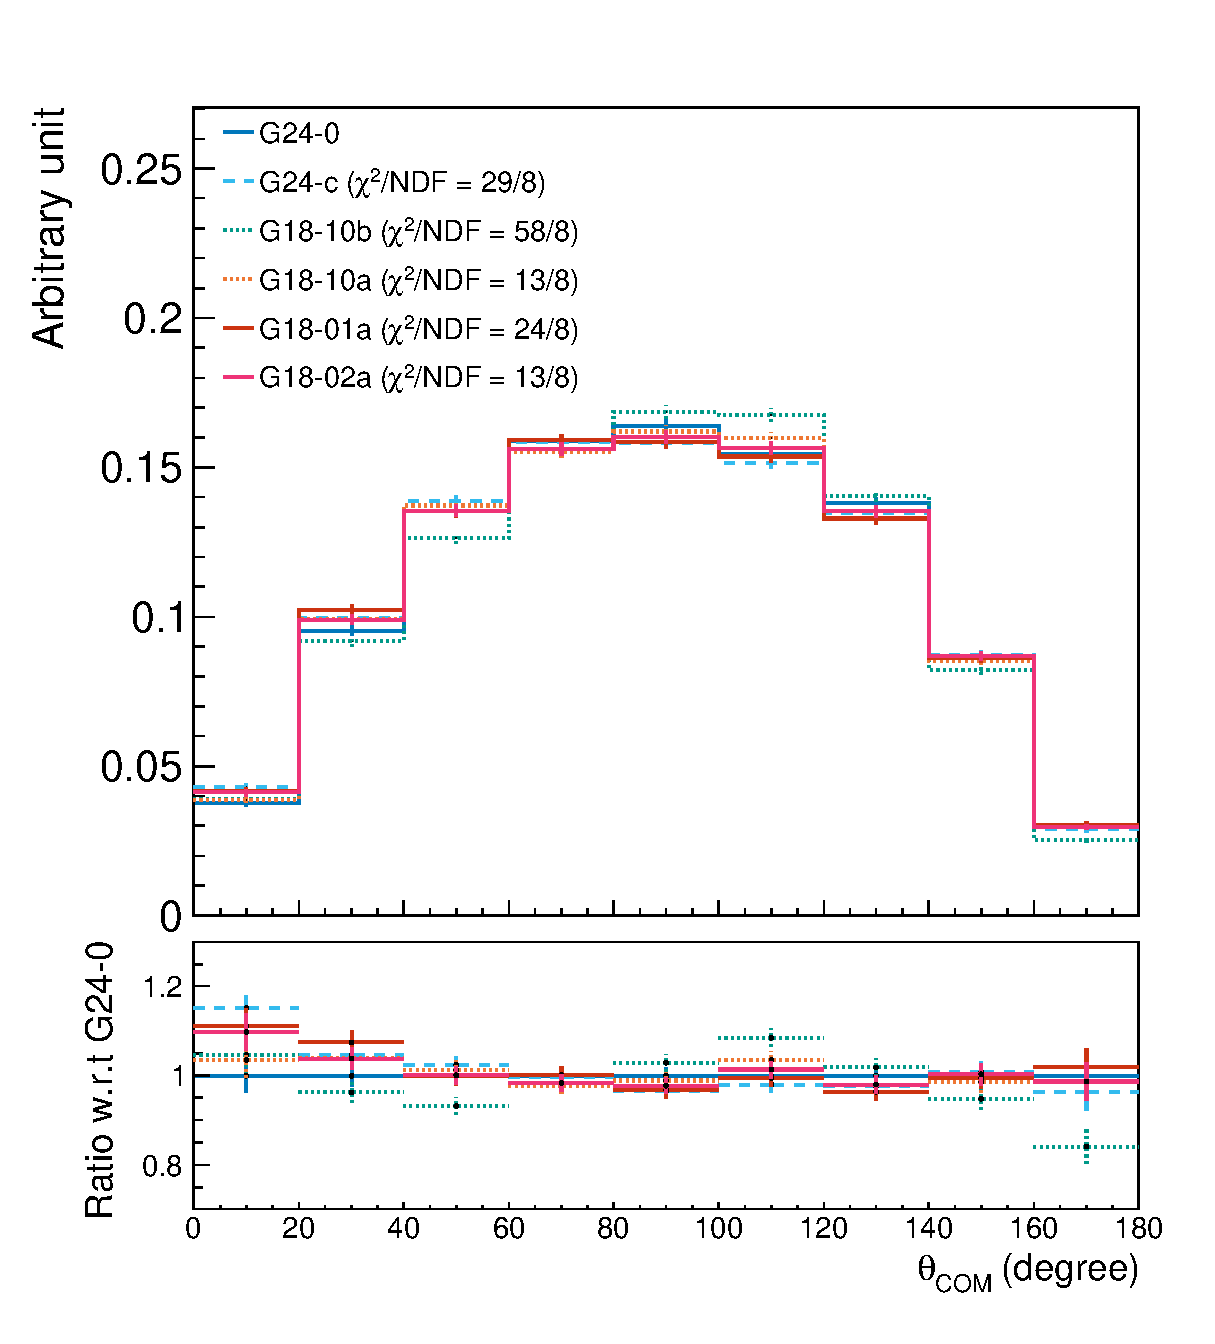
\includegraphics[width=\scfigwid\textwidth]{figures/COM/anorm-mod-ratio_da_tan.eps}
          % \caption{}
          % \label{subfig:mod-comp-ratio}
     % \end{subfigure}
     \caption{$\thetacom$ distribution comparisons using the T2K flux on carbon with multiple \genie configuations. }
     \label{fig:mod-comp}
     \end{figure}

     Notably, the configurations differing in their FSI model—\gC (tuned hA) and \getb (hN)—exhibit the largest $\chindf$ values, $29/8$ and $58/8$, respectively.
     \gC differs from \gZero only in its FSI model, as discussed in Fig.~\ref{subfig:g240c-comp-t2k}.
     In addition to differing in the FSI model, \getb also differs from \gZero in its IS and 2p2h models.
     In contrast, \geta—which shares the same FSI model as \gZero but differs in IS and 2p2h models in a manner similar to \getb—exhibits a much smaller $\chindf$ value of $13/8$, providing strong evidence that FSI is the primary reason for the large deviation observed in \getb relative to \gZero.

     Furthermore, \geoa and \getwoa differ from \gZero in additional model components, yet both exhibit relatively small $\chindf$ values.
     In particular, \getwoa is statistically compatible with \gZero—with a $\chi^2/\textrm{NDF}$ of $13/8$—despite differences in its IS, QE, and 2p2h models.
     While a change in the RES model alone does not impact $\thetacom$, as illustrated by the comparison between \geoa and \getwoa in Fig.~\ref{fig:0102a-comp}, the combined modifications in QE, IS, and 2p2h models cause \geoa to deviate further from \gZero, yielding a $\chindf$ of $24/8$.

     This comparison between different \genie tunes demonstrates that $\thetacom$ is most sensitive to changes in FSI while remaining robust against variations in other model components.
     A change in the RES model combined with modifications in other components can result in a noticeable alteration of the $\thetacom$ distribution, whereas a change in the RES model alone does not appear to have a significant impact.


     \subsection{Discussion}
     \label{sec:dis}
     The simulation studies in this work demonstrate that the COM angle is a novel variable with multiple advantages, and its measurement will be valuable for a focused study on FSI with minimal influence from other aspects of neutrino–nucleus interactions.
     Models constrained by $\thetacom$ measurements—e.g., following the methodology in Ref.~\cite{GENIE:2021zuu}—will remain relevant even if other aspects of neutrino–nucleus interactions, in particular the IS model, are updated in the future.
     This is an advantage that variables—such as $\thetaadt$, which depend on multiple processes of neutrino–nucleus interactions—do not possess.
     Furthermore, the analyses presented are based on true information without realistic fluctuations, meaning that challenges related to reconstruction—particularly those involving neutrino energy for the Adler angle—are not accounted for, whereas $\thetacom$ exhibits minimal dependence on neutrino energy reconstruction for T2K, as shown in Fig.~\ref{subfig:enu-comp-dpp-c}.
     Therefore, the full potential of the COM angle will be better realized in a cross-section measurement that accounts for these complexities.

     Although the focus of the $\thetacom$ analysis is on nuclear effects, it is inherently affected by resonance interaction modeling.
     Fortunately for T2K, resonance production is dominated by the $\deltapp$, thereby rendering the $\deltapp$ measurement at T2K resistant to changes in RES modelling, as shown in Fig.~\ref{fig:ma-comp} and Fig.~\ref{subfig:0102a-comp-t2k}.
     In contrast, the more energetic MINERvA flux produces multiple resonances, and the $\thetacom$ measurement is more sensitive to changes in RES modelling, as shown in Fig.~\ref{fig:ma-comp-minerva}.
     This sensitivity to RES modeling can be managed or even exploited in different ways.

     Firstly, imposing a cut on $\ecom$ to select $\deltapp$ events can reduce this sensitivity, as shown in Fig.~\ref{subfig:ma-comp-minerva-wcut} and Fig.~\ref{subfig:0102a-comp-minerva}, and under this condition, the $\thetacom$ measurement can be used for focused studies of FSI, similar to the T2K case.
     Secondly, comparing the $\thetacom$ distributions with and without the $\ecom$ cut can be used to study the onset of higher resonances and the correlations among different resonances.

     As noted in Sec.~\ref{sec:com}, the $\thetacom$ distribution is influenced by the production of higher resonances that decay via the same channels as $\deltapp$.
     Due to the general difference between $\thetaR$ and $\thetapidel$, $\thetacom$ will start to deviate from $\thetapidel$ (smeared by FSI), as shown in Fig.~\ref{subfig:enu-comp-cc1pi1p}.
     Although $\thetacom$ is inspired by $\thetapidel$, it is not restricted to the reconstruction or estimation of $\thetapidel$. 
     Rather, by definition, $\thetacom$ is a superposition of all energetically accessible $\thetaR$, with $\thetapidel$ as the dominant component at low energy.
     If all $\thetaR$ values are relatively well understood, a simple, theoretically motivated expectation of $\thetacom$ can be obtained by summing the contributions from all possible resonances according to their relative production ratios.

     This approach is complicated further by the fact that even with a complete understanding of the FSI model, the predicted $\thetacom$ distribution may deviate from measurements due to correlations among different resonance production modes; that is, the overall $\thetacom$ is not simply a linear combination of the individual $\thetaR$ contributions.
     Modeling of such correlations is currently absent in the BS model but is accounted for in the MK model~\cite{Kabirnezhad:2017jmf,Kabirnezhad:2020wtp,Kabirnezhad:2022znc}.
     Therefore, when the MK model is implemented and validated in the future, $\thetacom$ can be used to study these resonance correlations.
     This is particularly important for DUNE, where resonance production plays a major role.

     One limitation of using $\thetacom$ is that the FSI effects causing variations in the measured hadronic kinematic distributions are entangled with resonance effects.
     Hence, for the most sensitive study of resonance correlations, $\nu$-H selections are most suitable, as shown in Fig.~\ref{fig:enu-comp-h}.

     Furthermore, $\thetacom$ measurements based on $\nu$-H selections can be compared directly between different fluxes, as shown in Fig.~\ref{fig:flux-comp}.
     If high-purity $\nu$-H selections are achieved, $\thetacom$ measurements can provide a valuable pivot for cross-experiment comparison.

     The importance of a high-purity $\nu$-H sample cannot be overstated.
     For example, such events provide a unique opportunity for precise measurements of the axial current—a property unique to neutrinos.
     These advantages have driven significant efforts to develop techniques for selecting a high-purity $\nu$-H sample, as demonstrated in Refs.~\cite{Lu:2015hea,MINERvA:2023avz,Baudis:2023tma}.
     While Refs.~\cite{Baudis:2023tma} and \cite{MINERvA:2023avz} focus on neutrino and antineutrino pion-less events, respectively, Ref.~\cite{Lu:2015hea} pertains to the same event topology as that used for the COM total energy.
     With new or future detectors—e.g., the SFGD and the 3DST of DUNE~\cite{DUNE:2021tad}—there is greater potential to implement novel techniques for selecting a high-purity $\nu$-H sample.
     To this end, the sensitivity of the COM frame to FSI can be leveraged not only to study FSI but also to select events with minimal FSI.
     Preliminary studies have shown that at the SFGD, a considerable number of carbon background events remain after optimal cuts on TKI variables—namely, $\dptt$ and $\dpt$.
     Adding a cut on $\ecom$ can remove a significant portion of these background events, thereby achieving higher purity.
     A more thorough investigation of this application of $\ecom$ is required to obtain a reliable assessment of the improvement in purity and will be explored in future studies.

     \subsection{Reconstruction Quality}
     \label{sec:com-reco}
     The above discussion assumes true information, with ideal particle kinematics and selection criteria. It is important to assess the practicality of this approach by evaluating the uncertainties in reconstructing the COM variables. Therefore, I calculated the COM variables using the $\numuccopiop$ selection, identical to that used for the TKI calculation above. The reconstruction results are presented in Fig.~\ref{fig:com-reco}.
     \begin{figure}
          \begin{subfigure}[b]{\dbfigwid\textwidth}
               \centering
               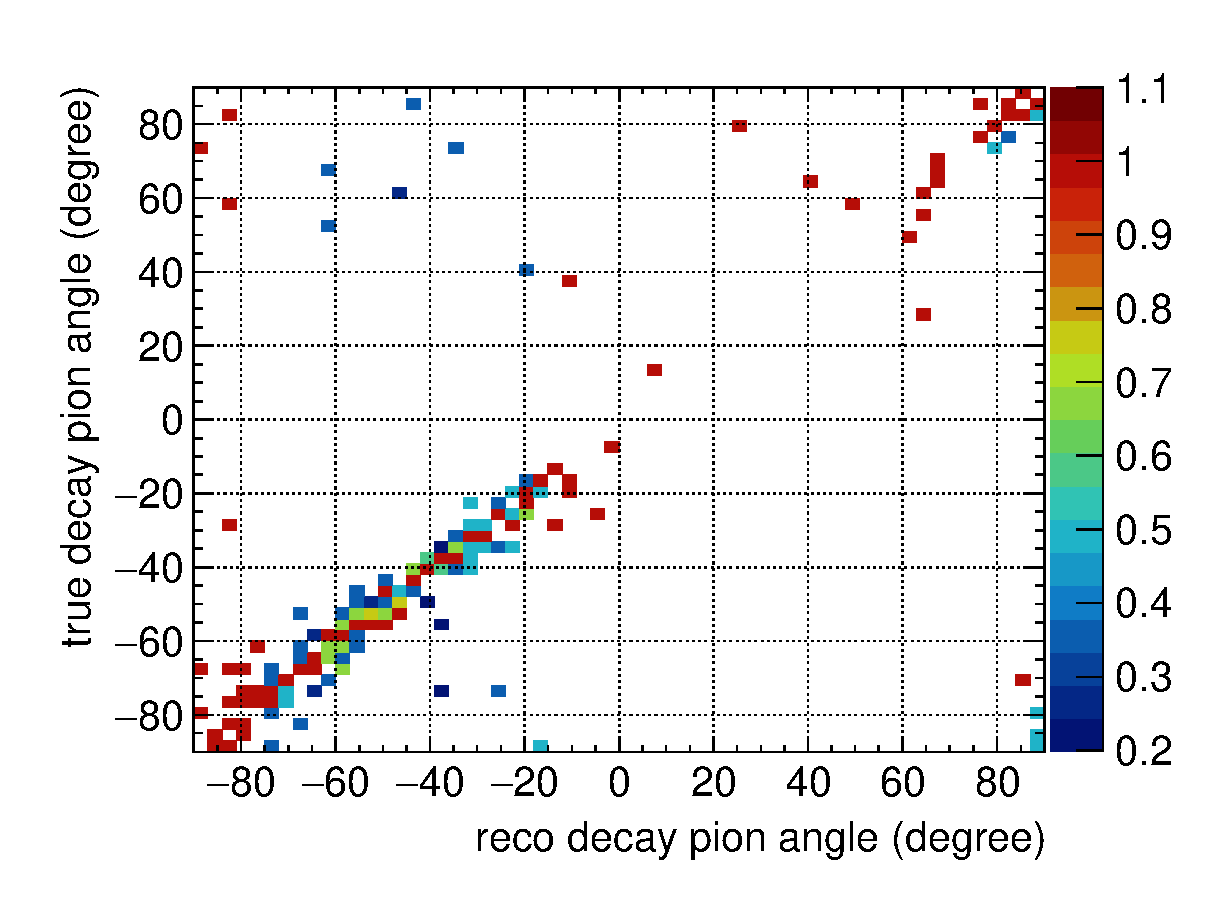
\includegraphics[width=\textwidth]{figures/COM/SFGpTPCmu_dang_colnor_resmat_al15.eps}
               \caption{$\thetacom$ Response Matrix}
               \label{subfig:reco-com-t-resmat}
          \end{subfigure}         
          \begin{subfigure}[b]{\dbfigwid\textwidth}
               \centering
               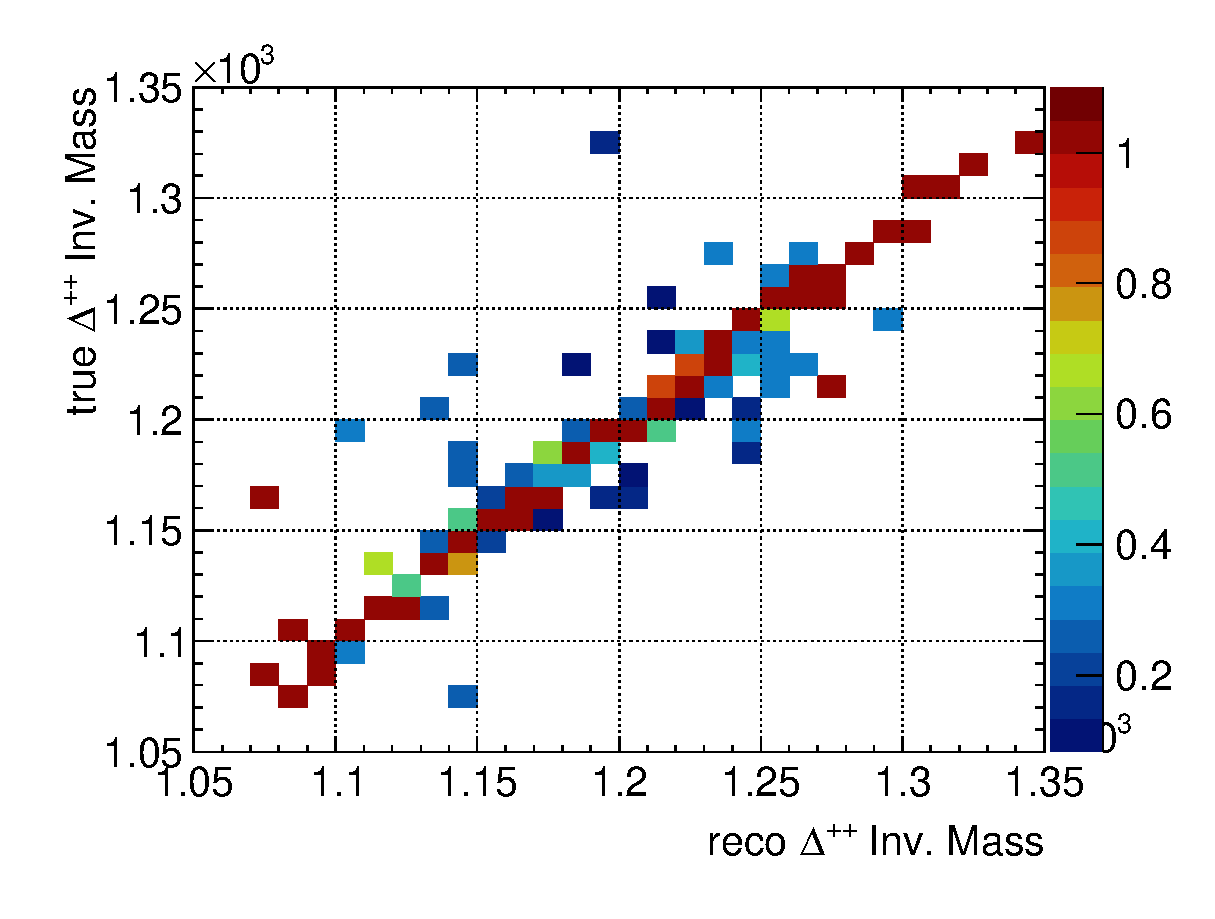
\includegraphics[width=\textwidth]{figures/COM/SFGpTPCmu_edelta_colnor_resmat_al15.eps}
               \caption{$\ecom$ Response Matrix}
               \label{subfig:reco-com-e-resmat}
          \end{subfigure}
          \\
          \begin{subfigure}[b]{\dbfigwid\textwidth}
               \centering
               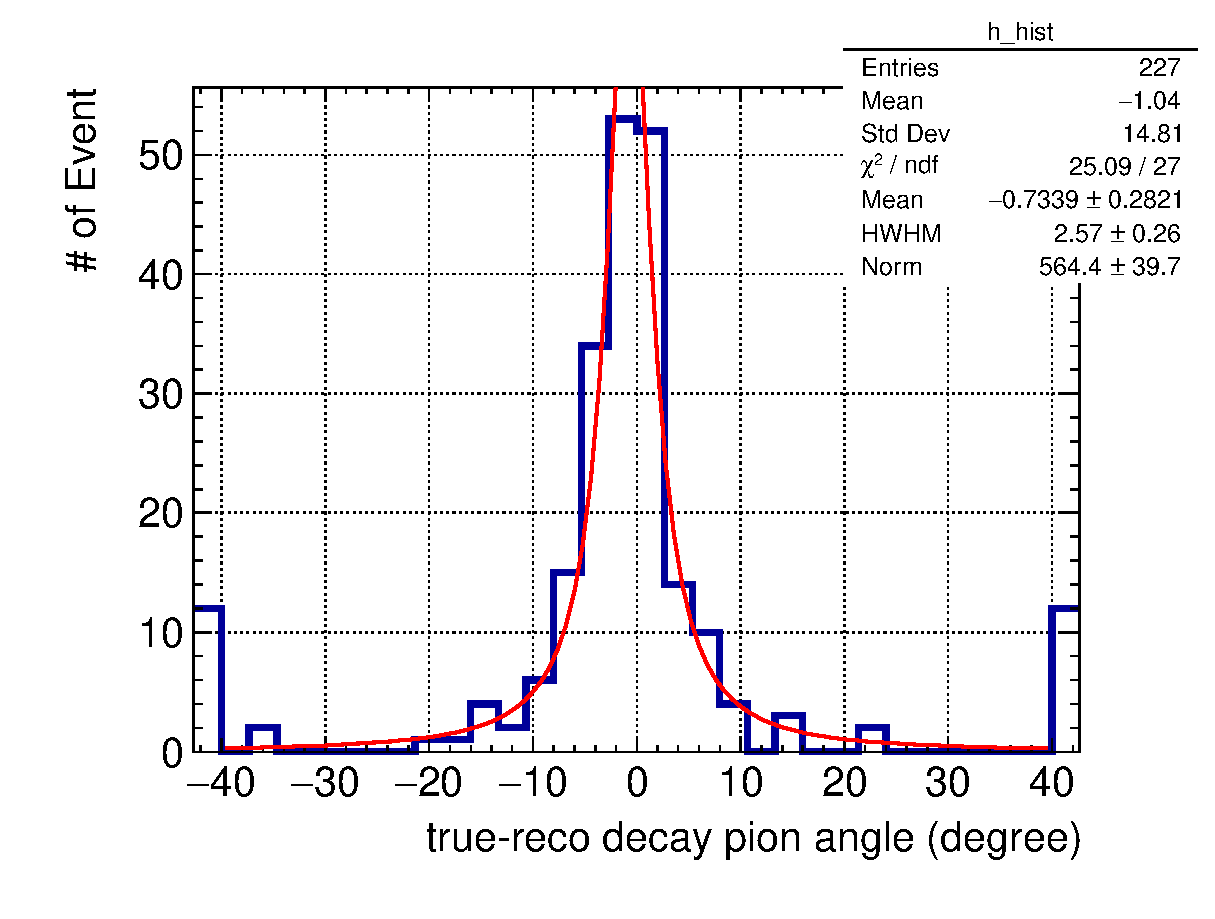
\includegraphics[width=\textwidth]{figures/COM/SFGpTPCmu_dang_res_hist_al15.eps}
               \caption{$\thetacom$ Resolution}
               \label{subfig:reco-com-t-res}
          \end{subfigure}
          \begin{subfigure}[b]{\dbfigwid\textwidth}
               \centering
               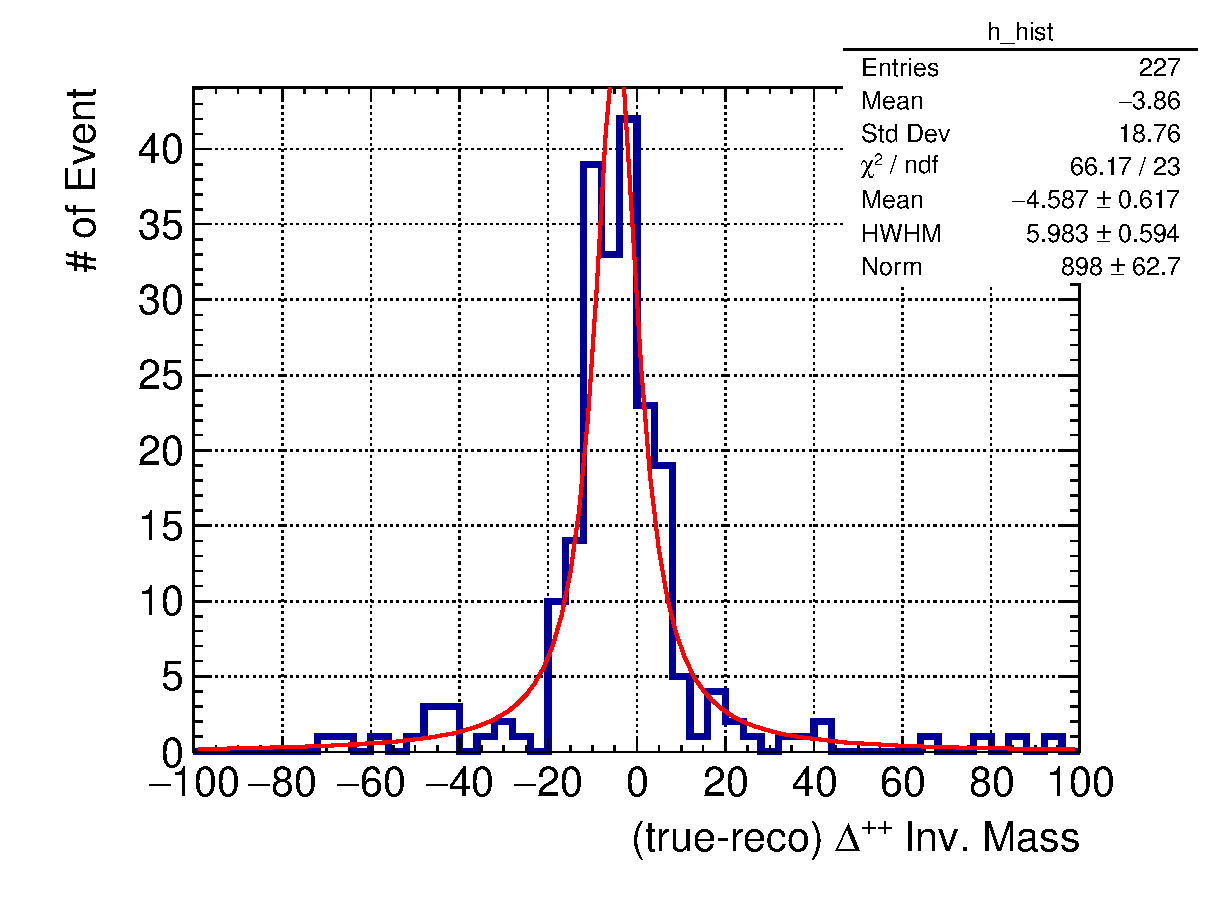
\includegraphics[width=\textwidth]{figures/COM/SFGpTPCmu_edelta_res_hist_al15.eps}
               \caption{$\ecom$ Resolution}
               \label{subfig:reco-com-e-res}
          \end{subfigure}
          \caption{COM variables for the $\numuccopiop$ selection.}
          \label{fig:com-reco}
     \end{figure}
     The analysis presented in Sec.~\ref{sec:com-ana} uses a binning of $20^\circ$ for $\thetacom$. In contrast, Fig.~\ref{subfig:reco-com-t-res} demonstrates that the reconstruction has an excellent half-width of $2.6^\circ$, significantly smaller than the analysis binning. This suggests that reconstruction will not impede the model differentiation capability discussed in Sec.~\ref{sec:com-ana} and may even enhance it due to the superb reconstruction quality of the SFGD. The fitted half-width of $\ecom$ is approximately $6.0~\mev$, which is also exceedingly precise. It will be more relevant for hydrogen sample selection, as discussed in the next section. 

     \subsection{Conclusion}
     This study introduces a novel set of variables—the COM angle and total energy. These variables possess several advantageous properties, which motivate their use in future cross-section measurements. Such measurements have the potential to significantly enhance our understanding and modeling of FSI processes in neutrino-nucleus interactions, thereby contributing to more accurate neutrino cross-section predictions. The reconstruction quality of the COM variables has been shown to be excellent, and it is promising that actual measurements can outperform the potential demonstrated in the true MC study.

\section{Hydrogen Sample Selection}
\label{sec:mc-hydrogen}
The sensitivity of the COM frame to FSI can be leveraged not only to study FSI but also to select events without FSI. 
These events are primarily composed of $\nu$-H interactions, which provide a unique opportunity for precise measurements of the axial current—a feature specific to neutrinos. 
Additionally, a $\nu$-H sample allows for the improvement of $\nu$-H modeling without the complications of IS and FSI, facilitating accurate neutrino energy reconstruction. 
These advantages have driven significant efforts to develop techniques for selecting a high-purity $\nu$-H sample, as seen in Ref.~\cite{Lu:2015hea,MINERvA:2023avz,Baudis:2023tma}.
While Ref.~\cite{Baudis:2023tma} and Ref.~\cite{MINERvA:2023avz} focuses on neutrino and antineutrino pion-less events respectively, Ref.~\cite{Lu:2015hea} applies to the same event topology as the COM total energy. 
They complement each other well.
The proposal in Ref.~\cite{Lu:2015hea} is to use $\dptt$ to select $\nu$-H events.
It is challenging to achieve high efficiency and purity with a one-dimensional cut. 
Therefore, a COM total energy cut is proposed to complement $\dptt$, and this section demonstrates its effectiveness.

\subsection{MC Study}
\label{sec:mc-hydrogen-ana}
     The key to removing carbon backgrounds from hydrogen events is to identify variables that effectively differentiate between the two.
     Therefore, distributions decomposed by target nucleus type are shown in Fig.~\ref{fig:hsel-tki-decomp} for the proposed variables.

     As shown in Fig.~\ref{subfig:hsel-dptt-stack}
     \begin{figure}
     \begin{subfigure}[b]{\dbfigwid\textwidth}
          \centering
          \includegraphics[width=\textwidth]{figures/perf/tki/SFGpTPCmu_dptt_stack_al15.eps}
          \caption{$\dptt$}
          \label{subfig:hsel-dptt-stack}
     \end{subfigure}
     \begin{subfigure}[b]{\dbfigwid\textwidth}
          \centering
          \includegraphics[width=\textwidth]{figures/perf/tki/SFGpTPCmu_dpt_stack_al15.eps}
          \caption{$\dpt$}
          \label{subfig:hsel-dpt-stack}
     \end{subfigure}
     \caption{Decomposed distributions for $\dptt$ and $\dpt$ for hydrogen and carbon events.}
     \label{fig:hsel-tki-decomp}
     \end{figure}
     Based on $\dptt$ alone, the most effective cut is $-10\mevc \leq \dptt \leq 30\mevc$.
     This cut yields 16 hydrogen events and 16 carbon events, for a purity of $50\%$.
     In comparison, Ref.~\cite{MINERvA:2023avz} reported ``5,580(180) signal events over an estimated background of 12,500 events,'' which corresponds to a purity lower than $50\%$ but a much larger total number of events.
     Hence, for the T2K sample to be most useful, maximizing purity is essential to minimize systematic uncertainties in parameter measurements.

     Because SFGD excels in 3D tracking, a cut on $\dpt$ may further reduce carbon backgrounds.
     A similar decomposition is shown in Fig.~\ref{subfig:hsel-dpt-stack} for $\dpt$.
     It is observed that $\dpt$ and $\dptt$ for hydrogen events cluster near $0$, while carbon events exhibit more spread.
     Since the variables are not entirely independent (because $\abs{\dptt} \leq \dpt$), identifying a suitable two-dimensional cut is simpler by plotting them together, as shown in Fig.~\ref{fig:hsel-dpt-dptt} for hydrogen and carbon separately.
     \begin{figure}
          \begin{subfigure}[b]{\dbfigwid\textwidth}
               \centering
               \includegraphics[width=\textwidth]{figures/perf/tki/SFGpTPCmu_dptt_colnor_vs_dpt_hist2d_al15_H.eps}
               \caption{Hydrogen events}
               \label{subfig:hsel-dpt-dptt-h}
          \end{subfigure}
          \begin{subfigure}[b]{\dbfigwid\textwidth}
               \centering
               \includegraphics[width=\textwidth]{figures/perf/tki/SFGpTPCmu_dptt_colnor_vs_dpt_hist2d_al15_C.eps}
               \caption{Carbon events}
               \label{subfig:hsel-dpt-dptt-c}
          \end{subfigure}
          \caption{Two-dimensional distributions of $\dpt$ and $\dptt$ for hydrogen and carbon events.}
          \label{fig:hsel-dpt-dptt}
     \end{figure}

     Fig.~\ref{fig:hsel-dpt-dptt} suggests the cuts, $\dpt < 80\mevc$ and $-40\mevc \leq \dptt \leq 30\mevc$, which lead to a sample of $19$ hydrogen events and $10$ carbon events, with a purity of $65.5\%$.
     This is the optimal purity and efficiency achievable by using TKI variables only.
     To further improve the purity, an additional cut on the COM variables is proposed.
     Similar to Fig.~\ref{fig:hsel-tki-decomp}, the decompositions for the COM variables are shown in Fig.~\ref{fig:hsel-com-decomp}.
     Although FSI alters the $\thetacom$ distributions, leading to distinct distributions between hydrogen and carbon, $\thetacom$ for hydrogen is expected to be uniform across the entire range; therefore, the cut on $\thetacom$ to select hydrogen is not expected to be effective.
     Note that to show the wide range of $\thetacom$ for hydrogen, the colours for hydrogen and carbon are switched in Fig.~\ref{subfig:hsel-com-theta} respectively.
     In contrast, without FSI, $\ecom$ is expected to center around the mass of the resonance, which is $1232~\mev$ for $\deltapp$, while the carbon events are expected to have a much wider distribution, as shown in Fig.~\ref{subfig:hsel-com-edelta}.
     \begin{figure}
     \begin{subfigure}[b]{\dbfigwid\textwidth}
          \centering
          \includegraphics[width=\textwidth]{figures/perf/tki/SFGpTPCmu_edelta_stack_al14.eps}
          \caption{$\ecom$}
          \label{subfig:hsel-com-edelta}
     \end{subfigure}
     \begin{subfigure}[b]{\dbfigwid\textwidth}
          \centering
          \includegraphics[width=\textwidth]{figures/perf/tki/SFGpTPCmu_dang_stack_al15.eps}
          \caption{$\thetacom$}
          \label{subfig:hsel-com-theta}
     \end{subfigure}
     \caption{Decomposed distributions for $\ecom$ and $\thetacom$ for hydrogen and carbon events.}
     \label{fig:hsel-com-decomp}
     \end{figure}
     Hence, an additional cut, $1168~\mev<\ecom<1257~\mev$ is implemented to further reduce the carbon backgrounds, achieving a sample of $18$ hydrogen events and $5$ carbon events, with an impressive purity of $78\%$.

     To demonstrate the effectiveness of these cuts, the $\dptt$ distributions are plotted step-wise in Fig.~\ref{fig:hsel-dptt-step}.
     Comparing the $\dptt$ distributions before and after each cut, namely the cuts on $\dpt$ and $\ecom$, it is evident that these cuts successfully remove carbon backgrounds in the low $\dptt$ region, which is impossible to remove based on $\dptt$ alone.
     Furthermore, by comparing Fig.~\ref{subfig:hsel-dang-dpt80} and Fig.~\ref{subfig:hsel-dang-dpt80-ecom}, it is demonstrated that the cut on $\ecom$ is capable of removing carbon backgrounds that cannot be removed by the transverse variables.
     Hence, all three variables are indispensable for achieving the optimal purity and efficiency.
     \begin{figure}
     \begin{subfigure}[b]{\trfigwid\textwidth}
          \centering
          \includegraphics[width=\textwidth]{figures/perf/tki/SFGpTPCmu_dptt_stack_al15.eps}
          \caption{No cut}
          \label{subfig:hsel-dang-nocut}
     \end{subfigure}
     \begin{subfigure}[b]{\trfigwid\textwidth}
          \centering
          \includegraphics[width=\textwidth]{figures/perf/tki/SFGpTPCmu_dptt_stack_al15_dpt80.eps}
          \caption{$\dpt < 80\mevc$}
          \label{subfig:hsel-dang-dpt80}
     \end{subfigure}
     \begin{subfigure}[b]{\trfigwid\textwidth}
          \centering
          \includegraphics[width=\textwidth]{figures/perf/tki/SFGpTPCmu_dptt_stack_al15_GetH_dpt80_wdang.eps}
          \caption{$\dpt < 80\mevc$ and $\ecom$ cut}
          \label{subfig:hsel-dang-dpt80-ecom}
     \end{subfigure}
     \caption{Step-wise $\dptt$ distributions for hydrogen and carbon events.}
     \label{fig:hsel-dptt-step}
     \end{figure}

     \subsection{Discussion}
     Both the transverse variables and $\ecom$ have limitations.
     The true distributions of the transverse variables on hydrogen are delta functions, but the dependence on an accurate neutrino direction reconstruction limits the reconstruction resolution of the transverse variables.
     The impact of the resolution is amplified as the cuts are placed to select events with small values when reconstruction uncertainties could relatively easily move the signal events out of the cut.
     On the other hand, while $\ecom$ has excellent reconstruction quality as it is independent of neutrino direction, its true distribution has a natural half-width of about $60~\mev$~\cite{ParticleDataGroup:2024cfk}.
     Hence, even if $\ecom$ can be reconstructed perfectly, it cannot separate hydrogen events from carbon events completely.
     Due to the limited amount of MC events available and the relatively small fraction of resonance events in the T2K beam, the statistics of the selection are too small to be conclusive.
     Nevertheless, the results are promising and suffice in demonstrating the complementarity of the transverse variables and $\ecom$.
     Hence, it is hopeful that using the two kinds of variables together, the upgraded ND280 data can produce a hydrogen sample with high purity.